\thispagestyle{only-cfoot}
\section{Evaluation}\label{s:Evaluation}

% \todo{Outline of experiment evaluation}

% robimy 3 zestawienia (Kube-sched, HEFT, PEFT) dla 3 workflow (SoyKB, Montage 0.25, Montage) w każdym subsection

This chapter presents the evaluation of the proposed concept of scheduling DAG-oriented workloads in Kubernetes and a comparison with the currently available solutions.
Three different experiment scenarios are thoroughly described and have their results analyzed in detail.

%%%%%%%
\subsection{Process description}\label{s:Evaluation:ProcessDescription}
% \todo{osobna subsection?}
The evaluation process revolves around three discussed scheduling approaches:

\begin{itemize}[topsep=0pt]
    \item{
kube-scheduler (without scheduler plugin) -- default solution,
}
    \item{
kube-scheduler with HEFT scheduler plugin,
}
    \item{
kube-scheduler with PEFT scheduler plugin.
}
\end{itemize}
A single scenario consists of ten individual runs of a workflow for every approach for each considered scientific application.
All cases have been repeated to mitigate the risk of comparing the results obtained from outliers.
The final results are averaged, then analyzed and compared considering the difference significance with a 95\% confidence level.


% Each scenario run was repeated ten times to results were averaged.
% To verify significance of the results, the metric values were
% The average values had their difference significance checked with a T test.

% negligible

%%%%%%%
\subsection{Static scheduling}\label{s:Evaluation:HyperflowScheduler}

% \todo{Evaluation without task clustering}

The first prepared scenario is workflow execution without task clustering.
Its results allow to analyze the effectiveness and applicability of traditional scheduling algorithms for containerized environments.
In this scenario, two scientific workflows are considered:

\begin{itemize}[topsep=0pt]
  \item{
SoyKB (52 time consuming tasks),
}
  \item{
Montage2-v0.25 (619 smaller tasks).
}
\end{itemize}
Both have been chosen for their relatively small size in terms of task number and short enough completion times for repetitive runs.


The example execution traces of SoyKB workflow are shown in \cref{fig:evaluation:sched:soykb} and the numerical values of calculated metrics are presented in \cref{tab:metrics-sched-soykb}.


%%%%%%%
% SoyKB traces
%%%%%%%
% \begin{figure}[H]
% \centering
% 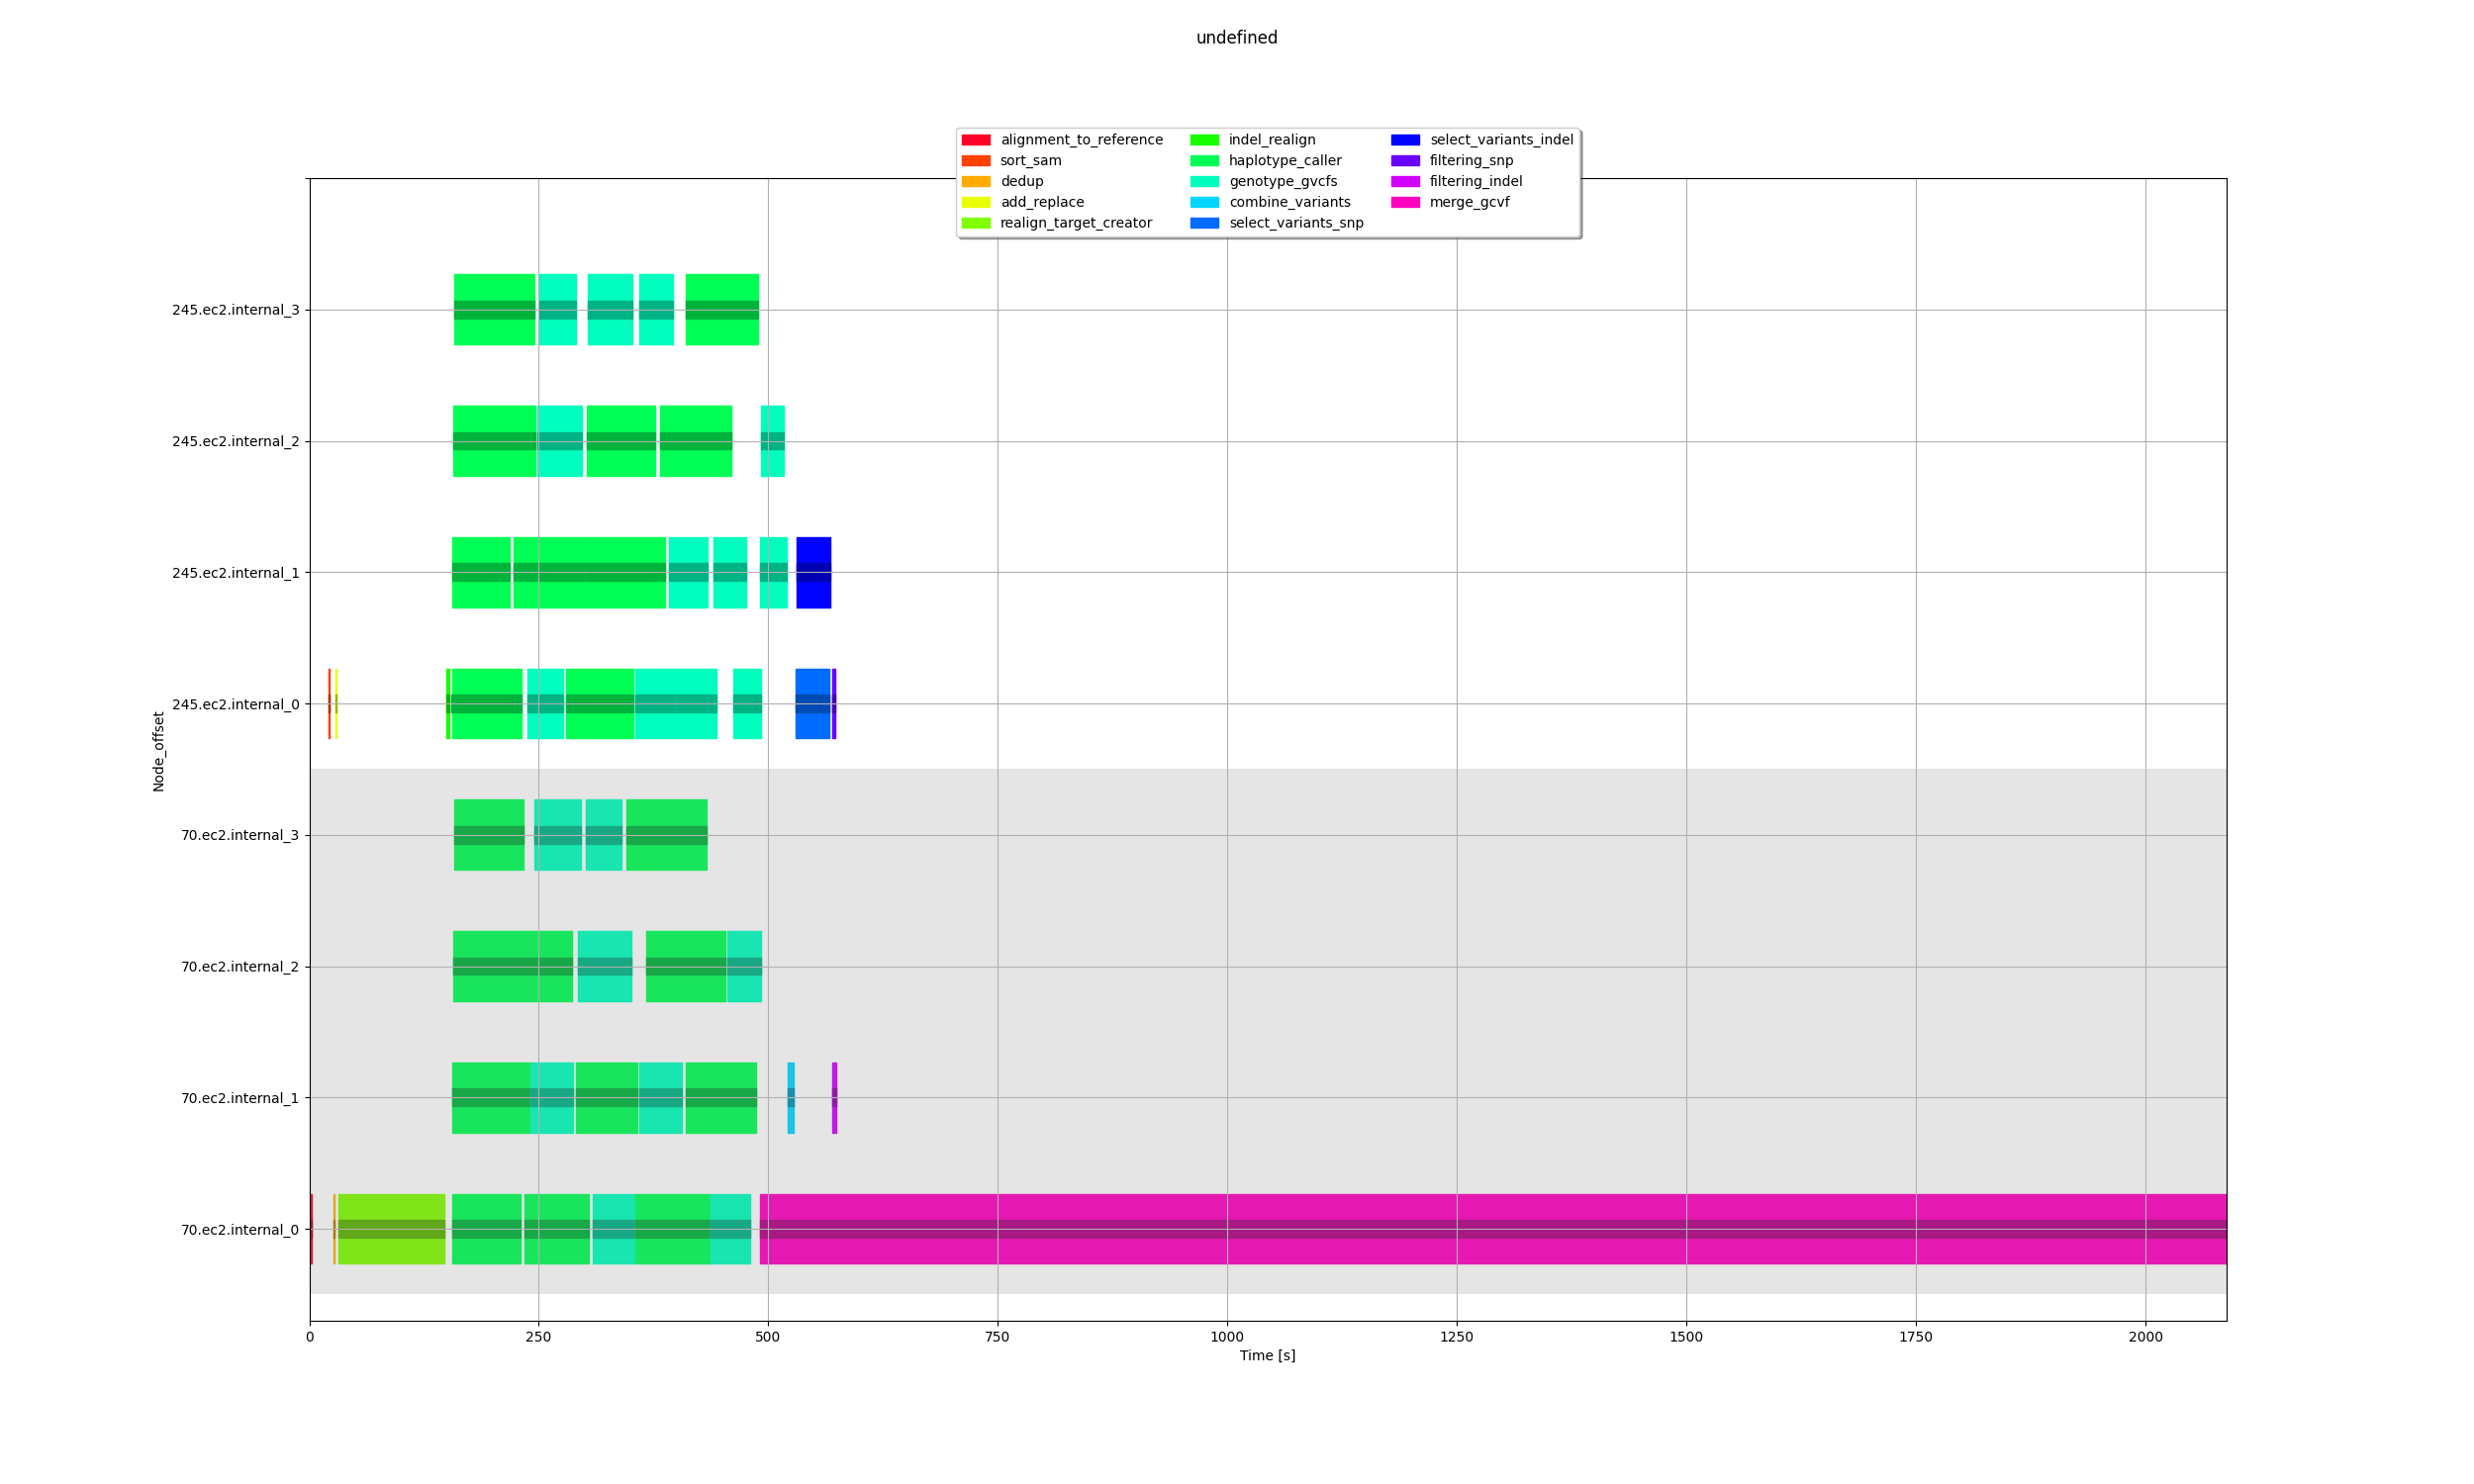
\includegraphics[width=1\linewidth]{figures/6-1-soykb-empty.png}
% %%
% \caption[Trace for sole kube-scheduler schedule on SoyKB]{Trace for sole kube-scheduler schedule on SoyKB.}
% \label{fig:evaluation:sched:soykb:empty}
% \end{figure}
% %%%%%%%
% \begin{figure}[H]
% \begin{subfigure}{1\textwidth}
% \centering
% 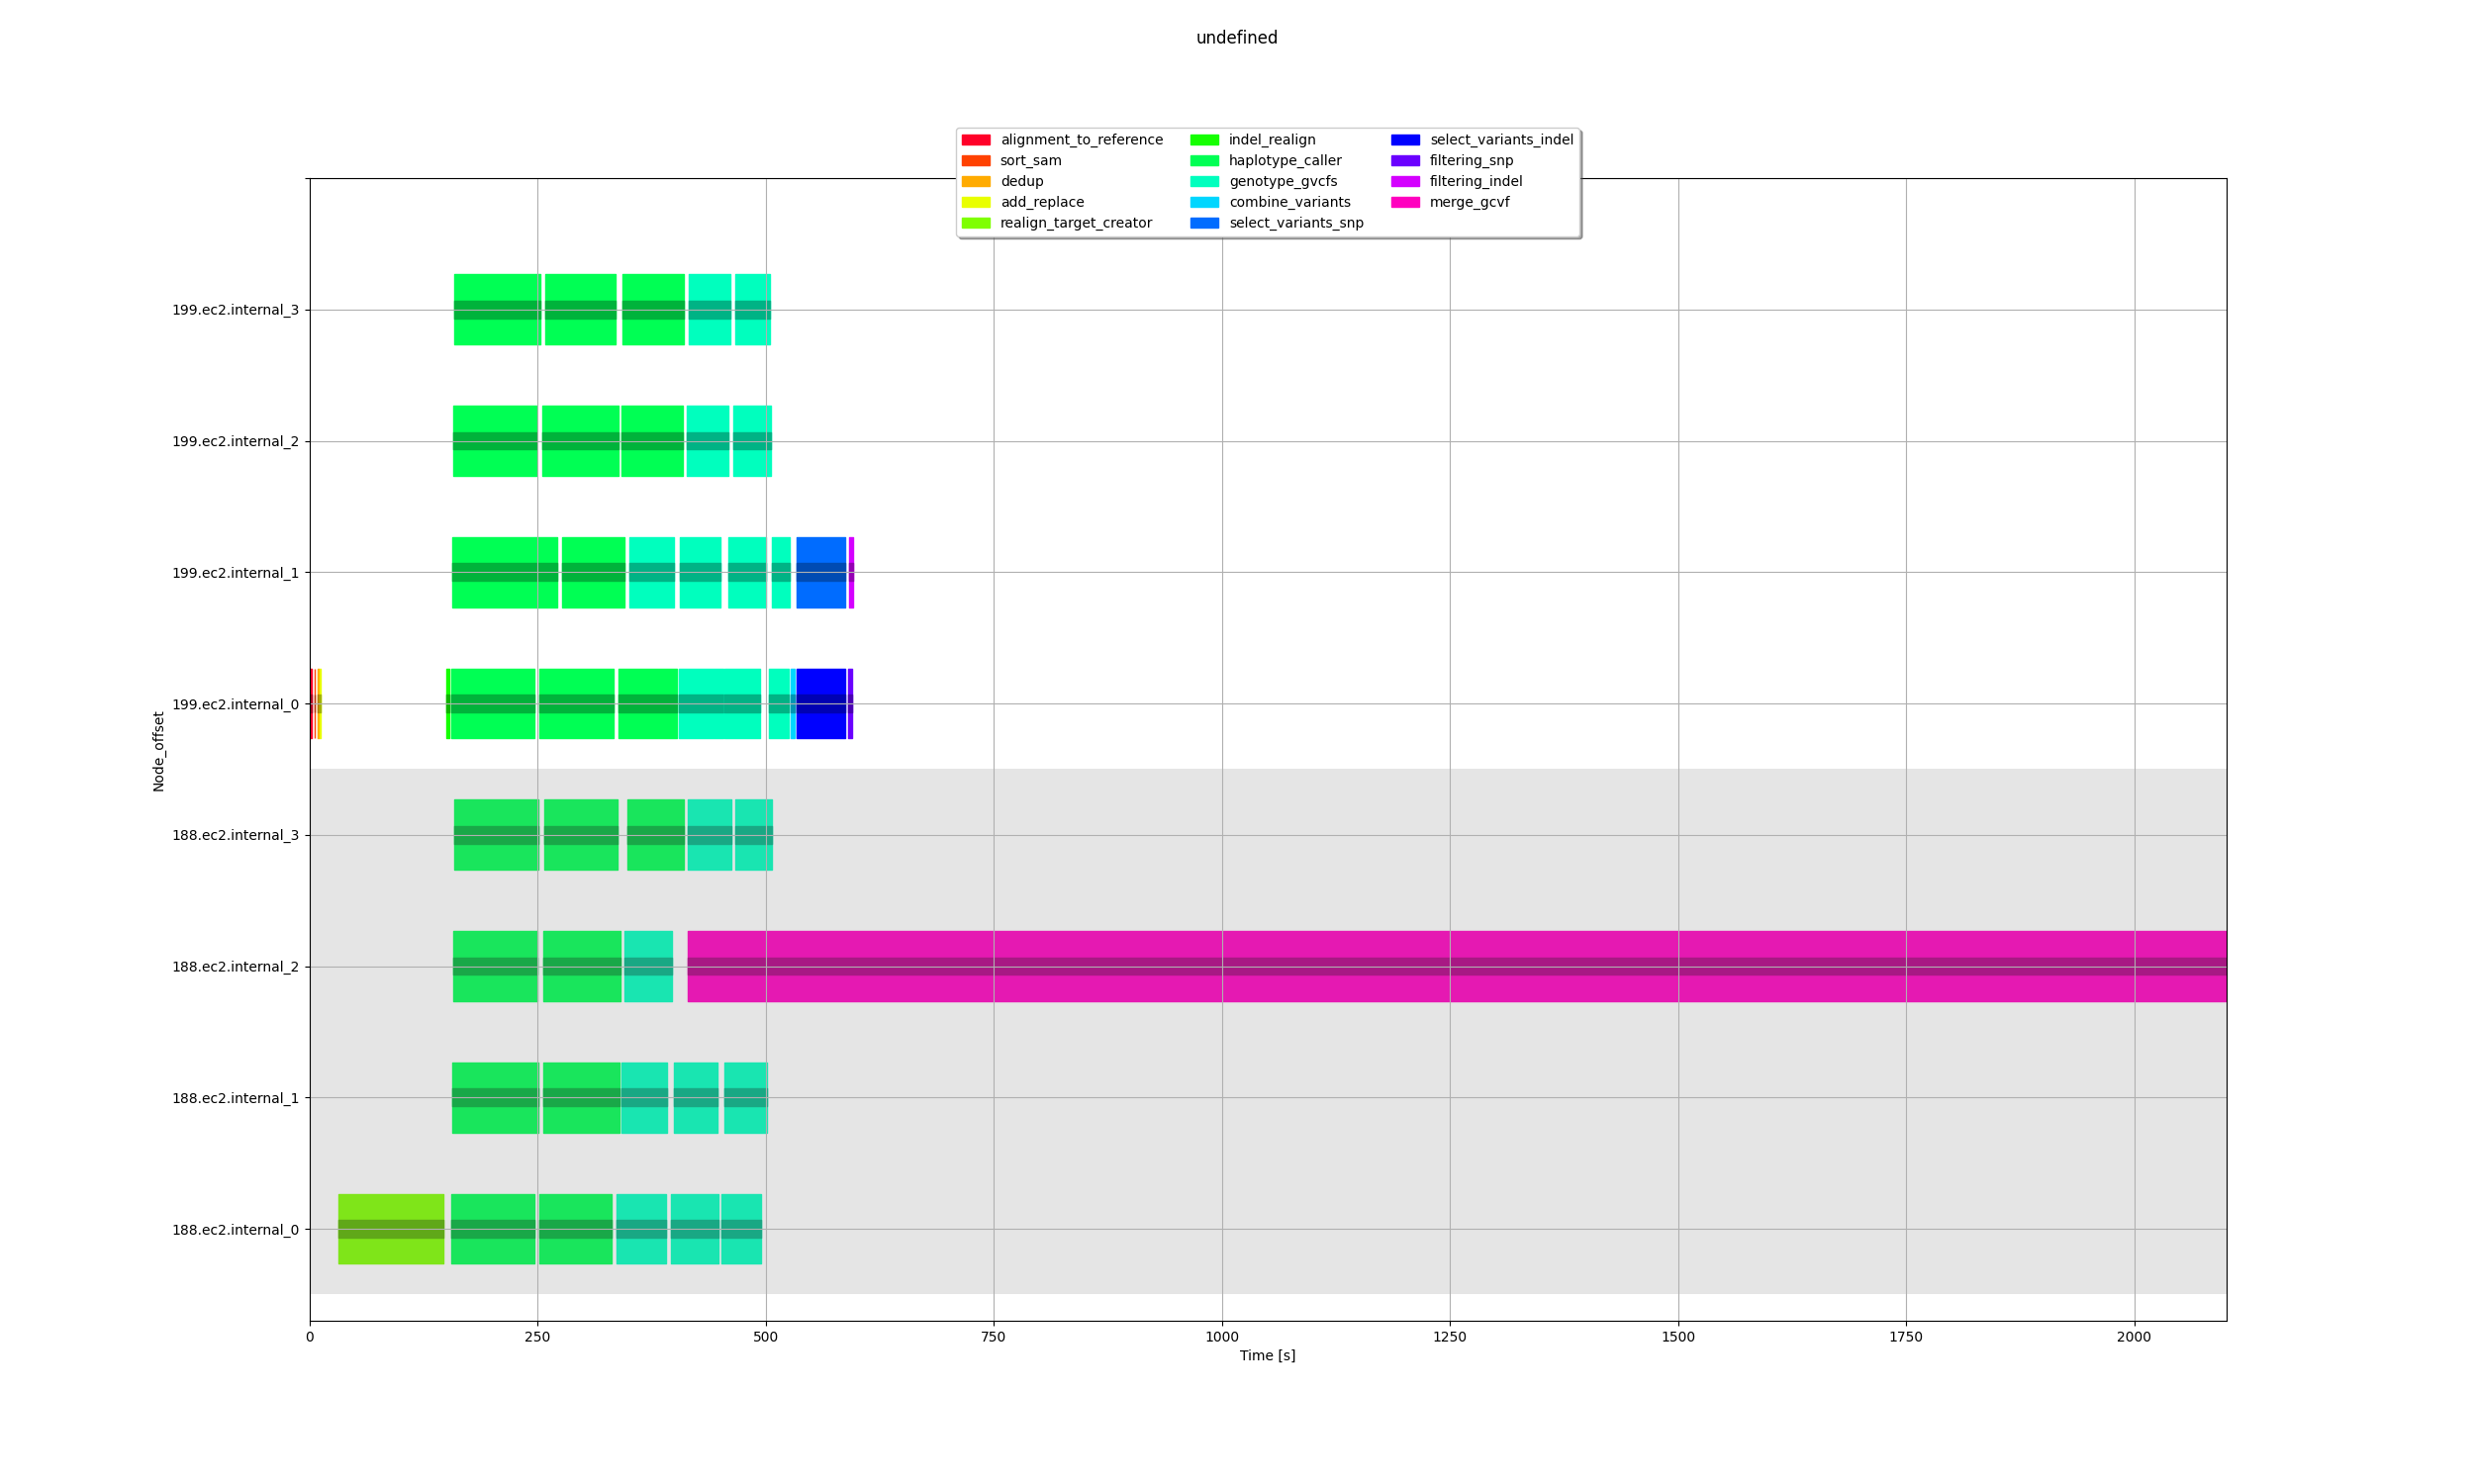
\includegraphics[width=1\linewidth]{figures/6-1-soykb-heft.png}
% \caption[Execution trace with HEFT scheduler plugin on SoyKB]{HEFT}
% \label{fig:evaluation:sched:soykb:heft}
% \end{subfigure}
% \begin{subfigure}{1\textwidth}
% \centering
% 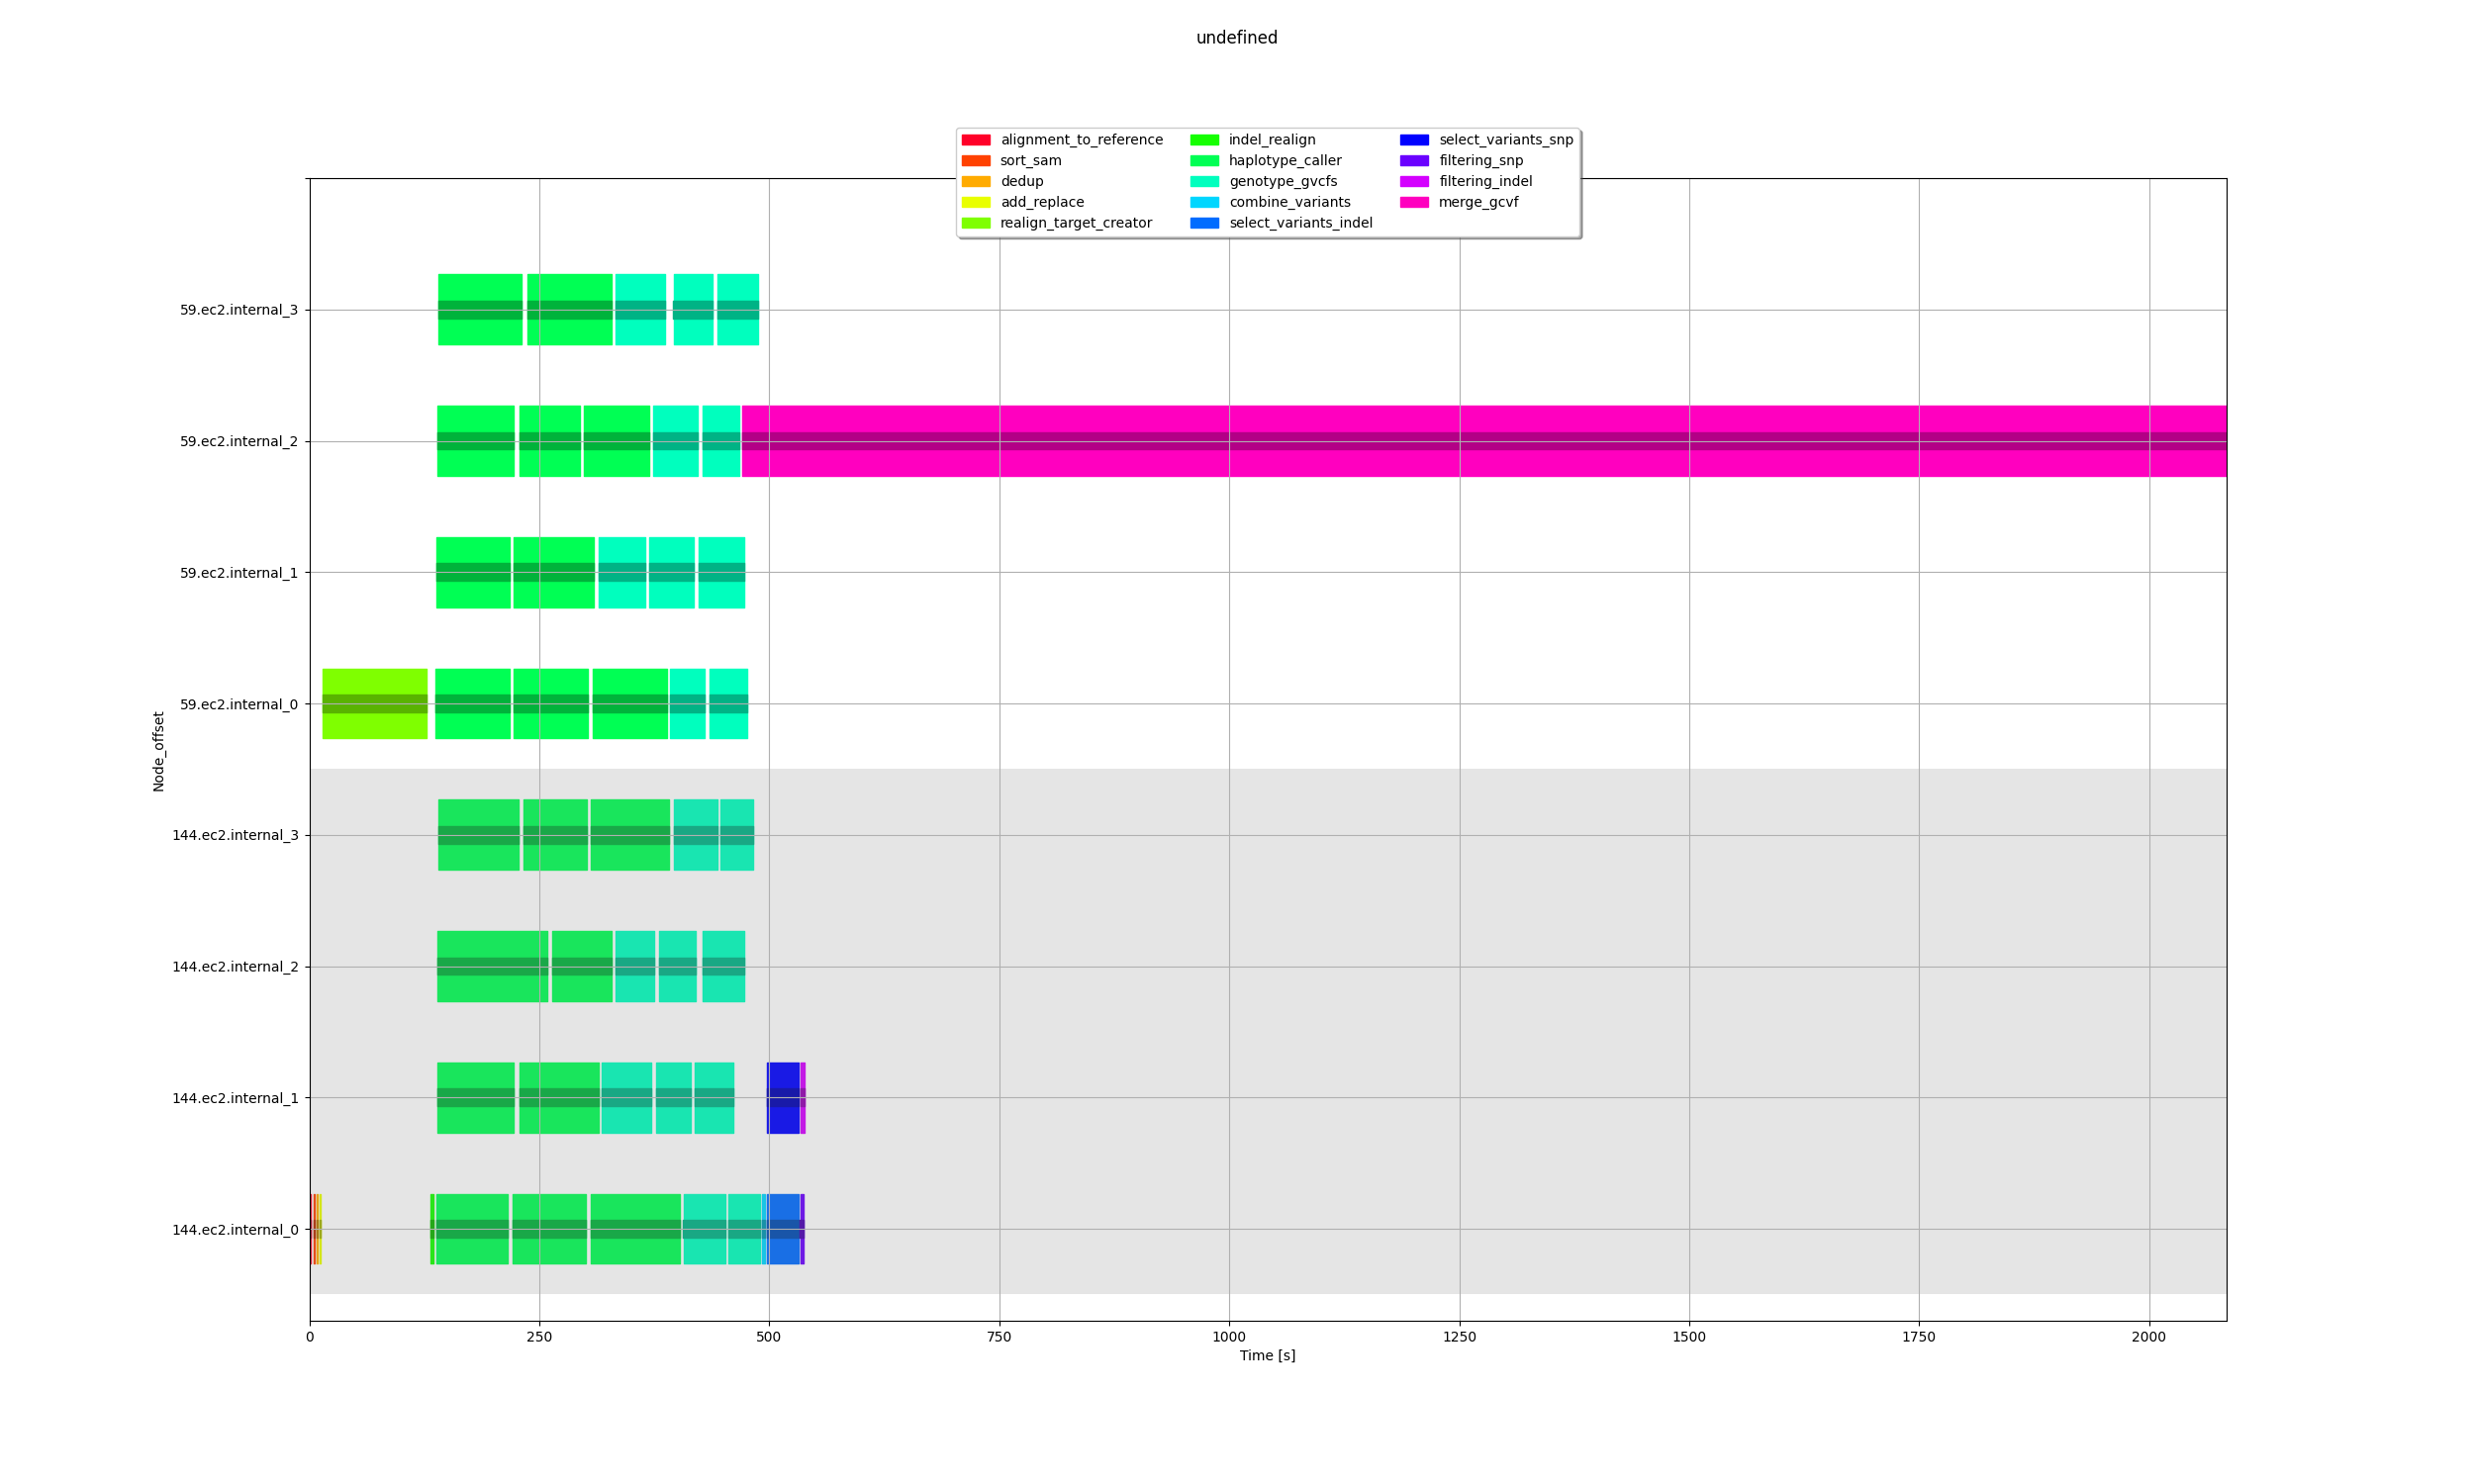
\includegraphics[width=1\linewidth]{figures/6-1-soykb-peft.png}
% \caption[Execution trace with PEFT scheduler plugin on SoyKB]{PEFT}
% \label{fig:evaluation:sched:soykb:peft}
% \end{subfigure}
% \centering
% %%
% \caption[Execution traces with scheduler plugin on SoyKB]{Execution traces with scheduler plugin on SoyKB.}
% %%
% \medskip
% \begin{minipage}{0.75\textwidth}
% {\footnotesize Blah blah \par}
% \end{minipage}
% %%
% \label{fig:evaluation:sched:soykb:plugin}
% \end{figure}

%%%%%%%

\begin{figure}[H]
\begin{subfigure}{0.75\textwidth}
\centering
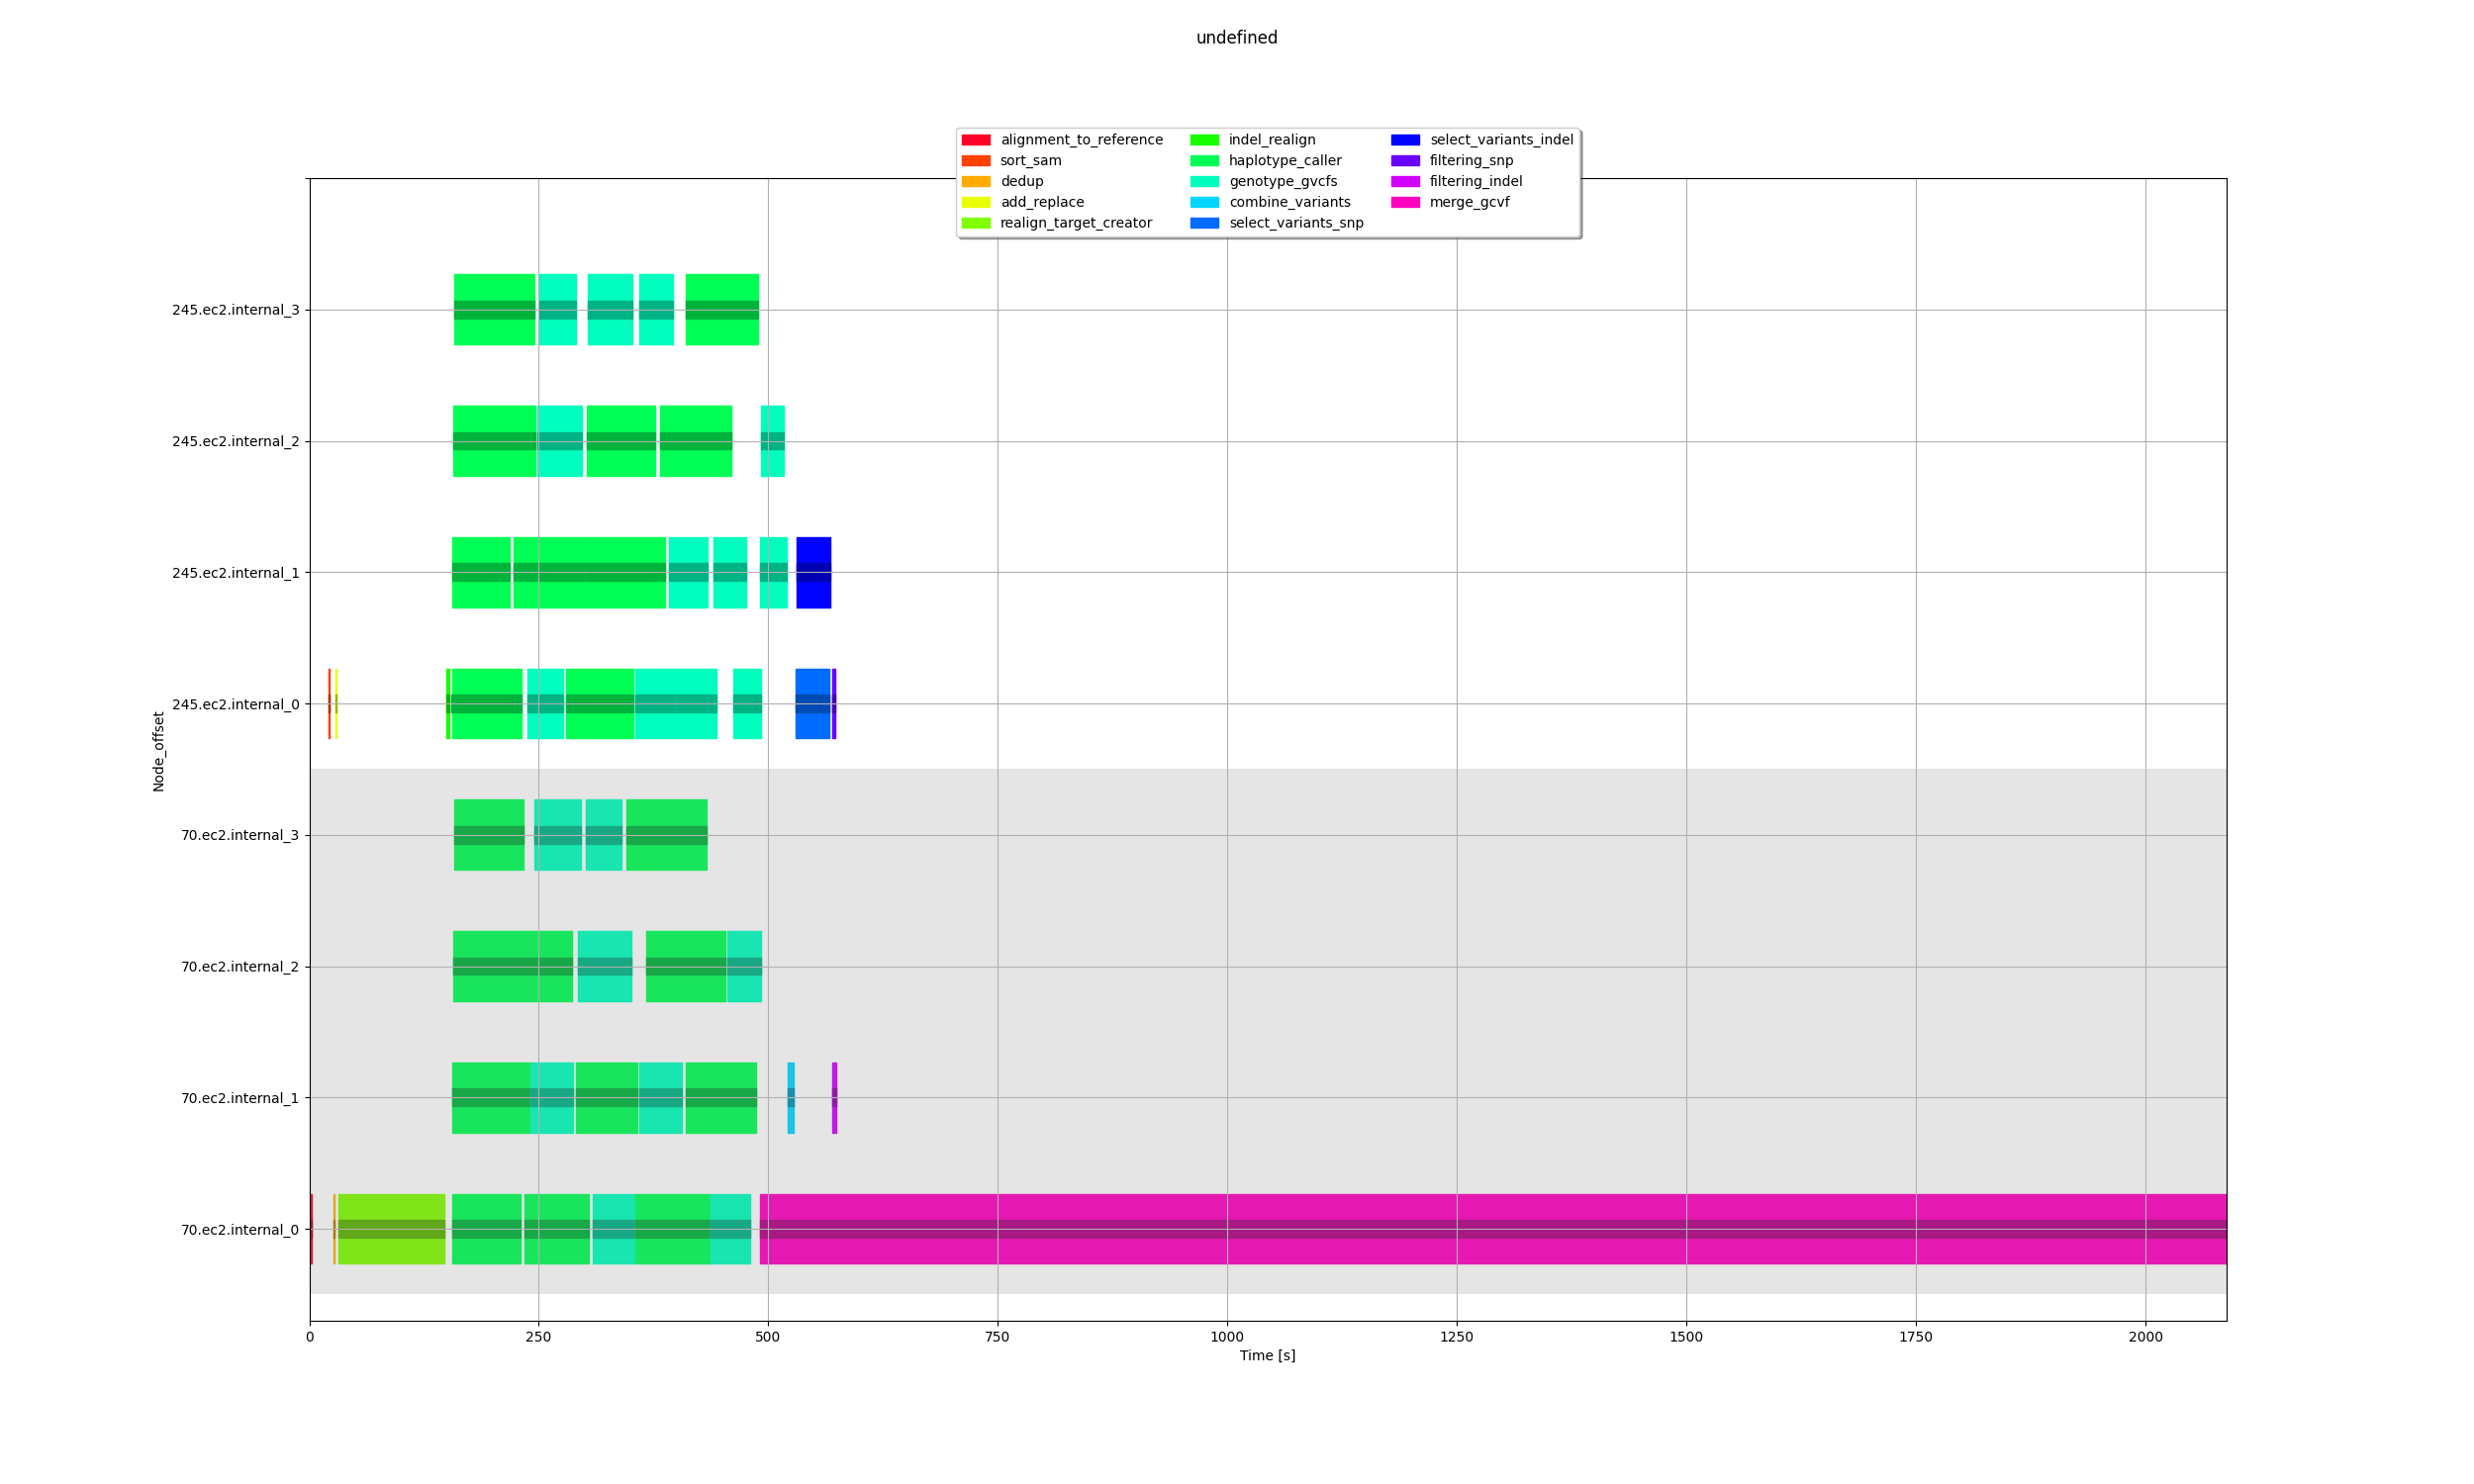
\includegraphics[width=1\linewidth]{figures/6-1-soykb-empty.png}
\caption[Selected example execution trace for SoyKB workflow without static scheduling]{w/o scheduler plugin}
\label{fig:evaluation:sched:soykb:empty}
\end{subfigure}
\begin{subfigure}{0.75\textwidth}
\centering
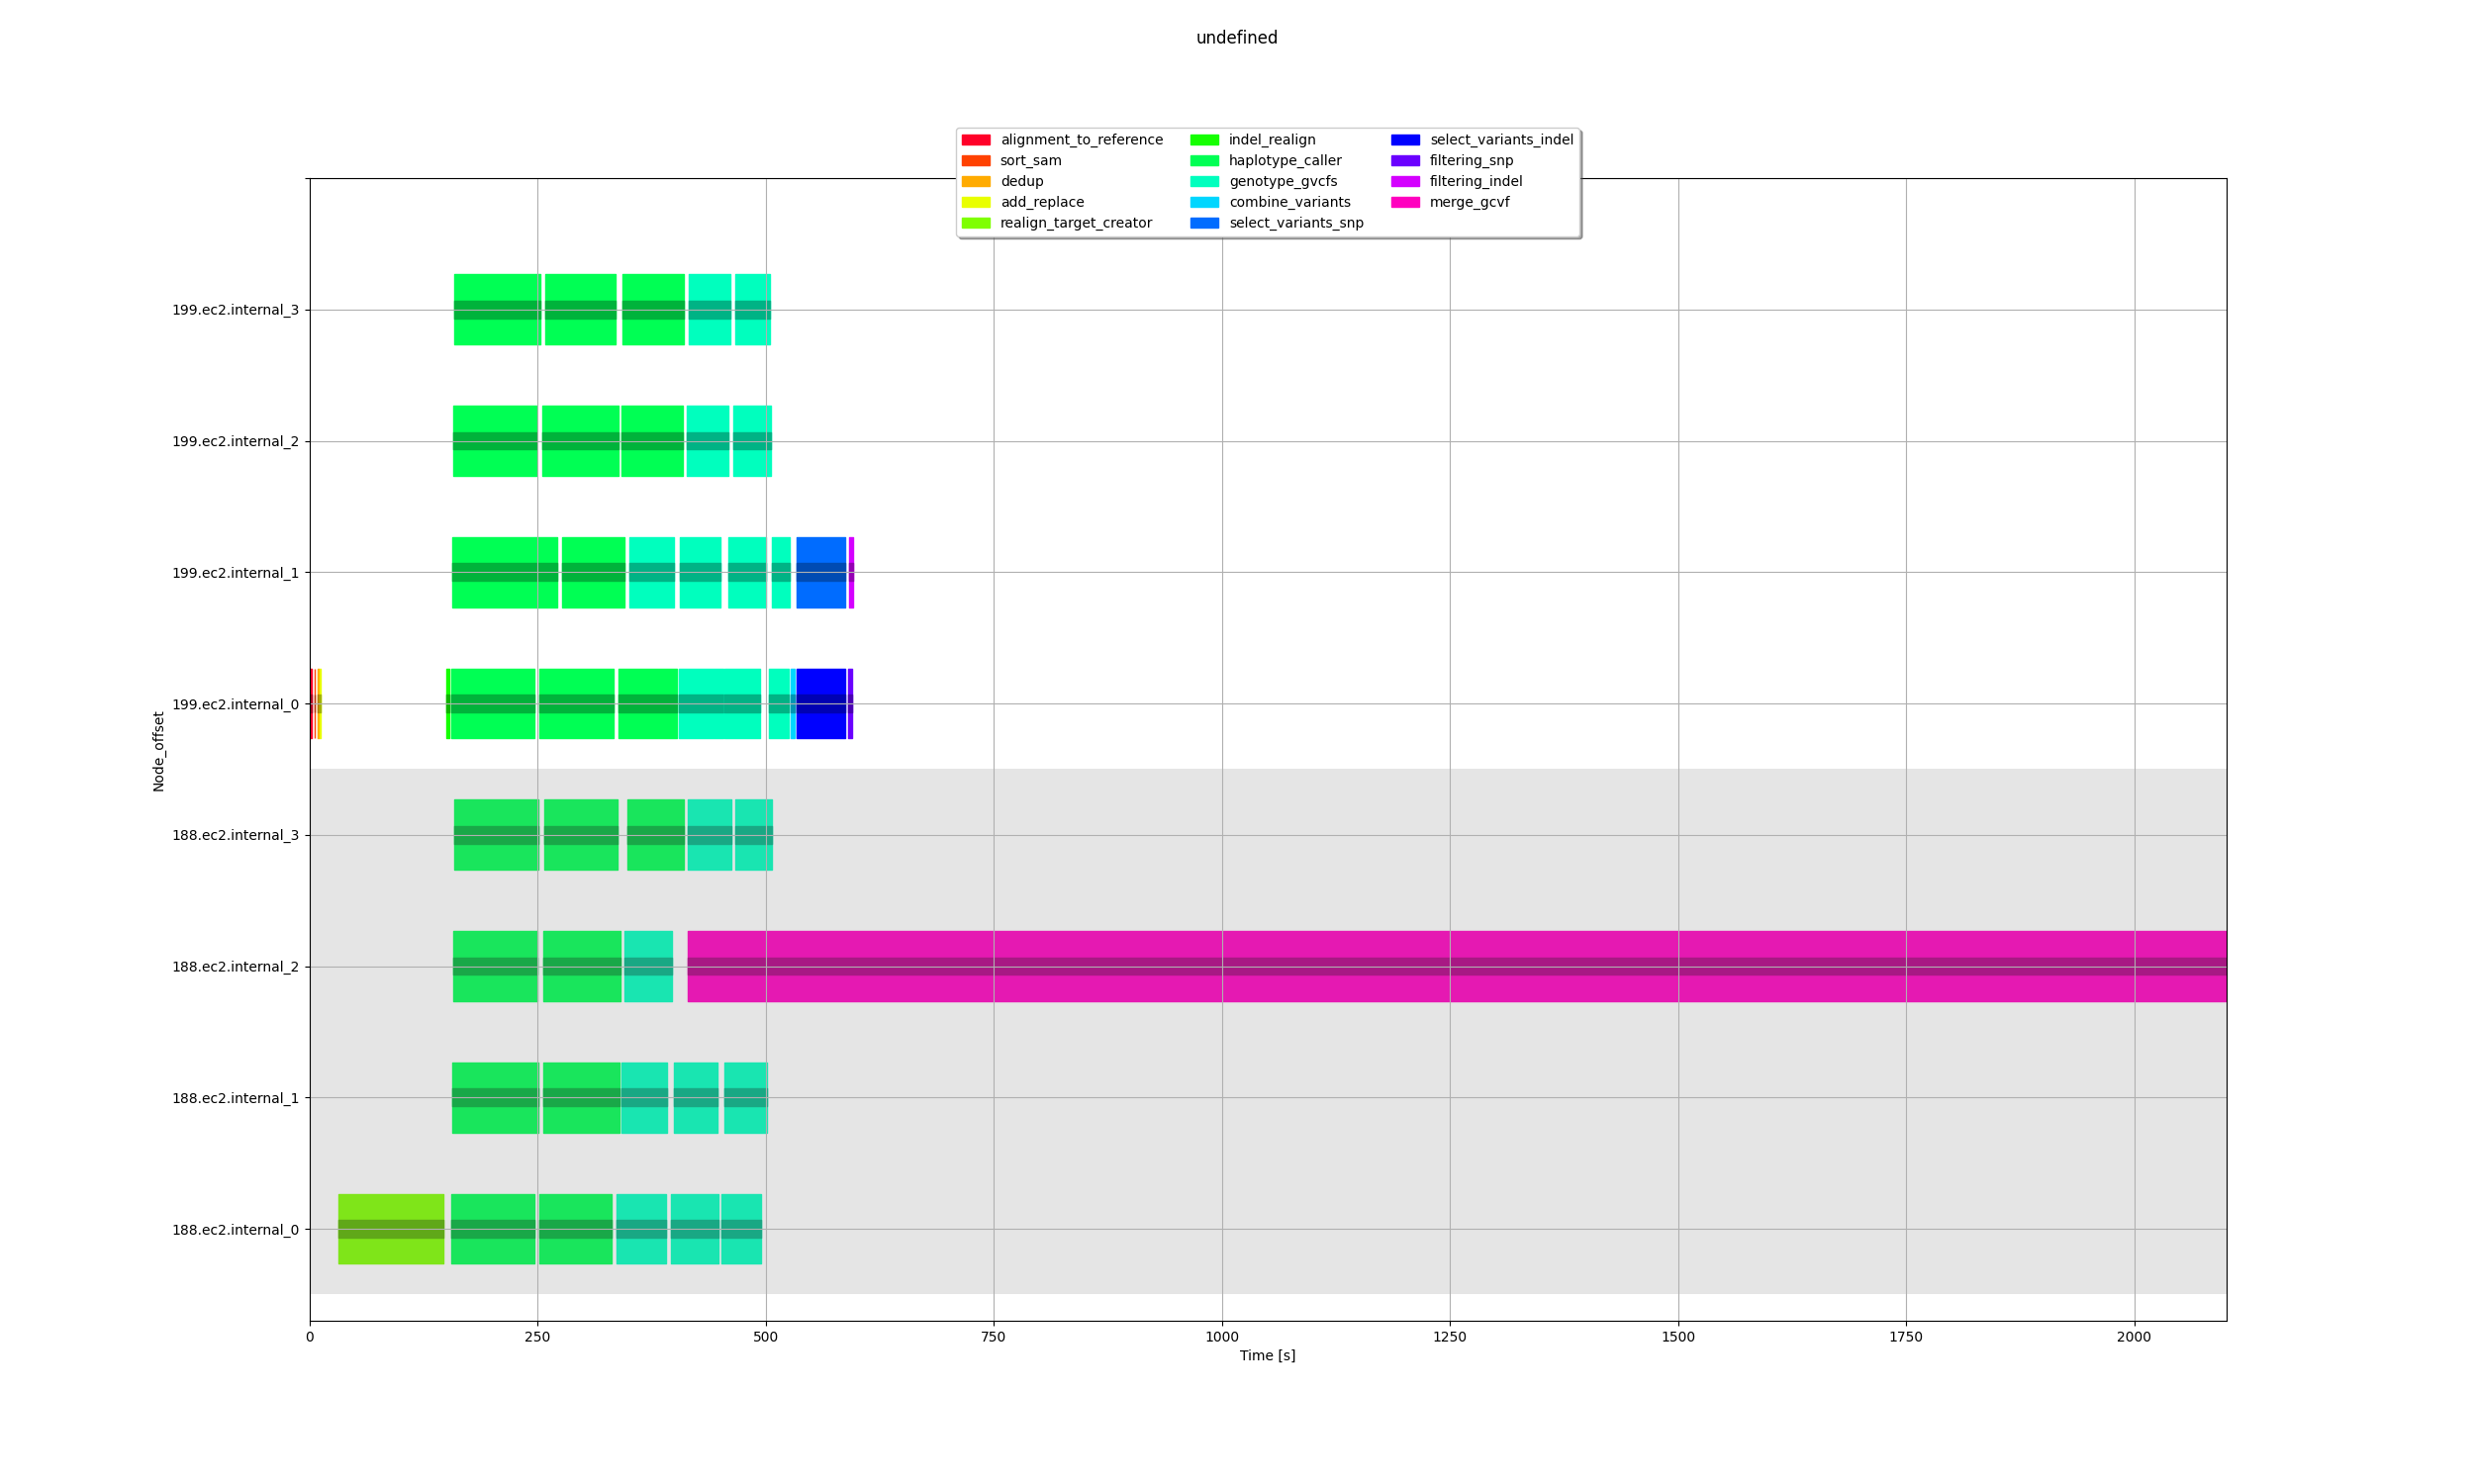
\includegraphics[width=1\linewidth]{figures/6-1-soykb-heft.png}
\caption[Selected example execution traces for SoyKB workflow with HEFT]{HEFT}
\label{fig:evaluation:sched:soykb:heft}
\end{subfigure}
\begin{subfigure}{0.75\textwidth}
\centering
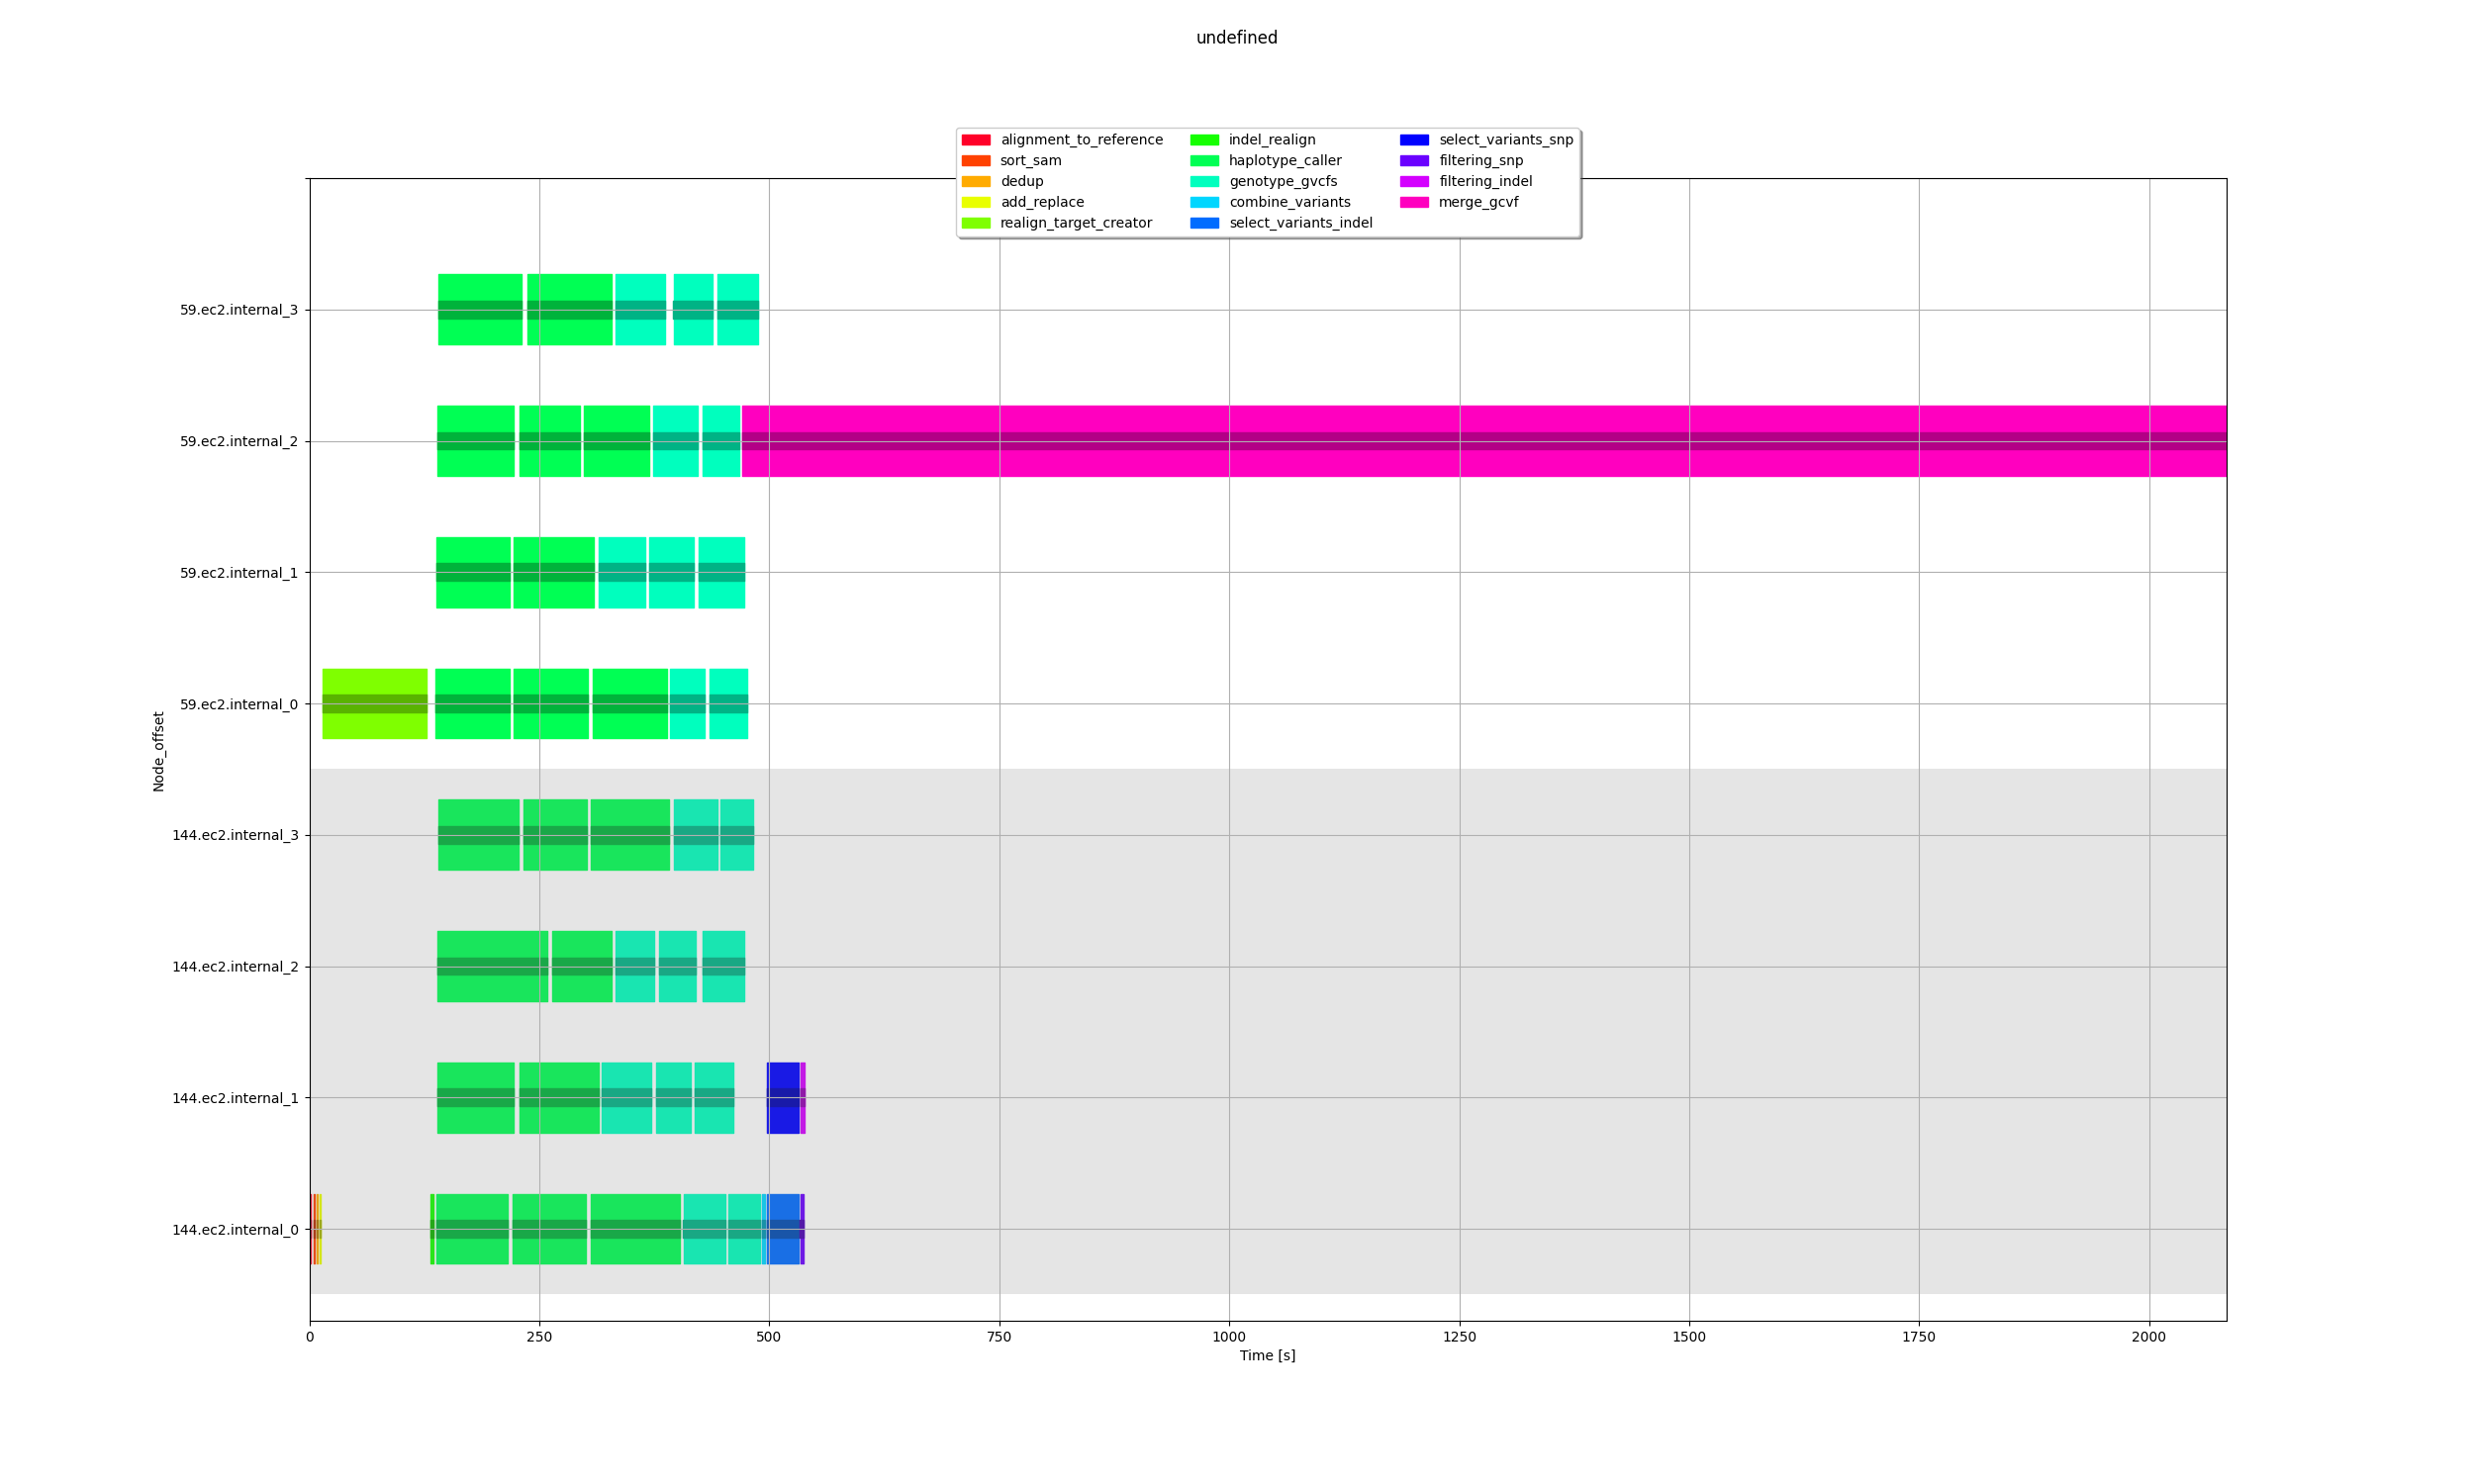
\includegraphics[width=1\linewidth]{figures/6-1-soykb-peft.png}
\caption[Selected example execution traces for SoyKB workflow with PEFT]{PEFT}
\label{fig:evaluation:sched:soykb:peft}
\end{subfigure}
\centering
%%
\caption[Selected example execution traces for SoyKB workflow]{Selected example execution traces for SoyKB workflow.}
%%
% \medskip
% \begin{minipage}{0.75\textwidth}
% % {\footnotesize Blah blah aaaaa aaaaa aaaaaaaaaaaaaaa aaaaa aaaaa aaaaaaaaaa aaaaaaaaaa aaaaa aaaaa aaaaa aaaaa aaaaa aaaaa aaaaa v v aaaaa aaaaa aaaaa aaaaa aaaaa \par}
% \end{minipage}
% \medskip
%%
\label{fig:evaluation:sched:soykb}
\end{figure}

%%%%%%%

%%%%
% Tabelka z metrykami - SoyKB
\begin{table}[H]
    \centering
    \begin{tabular}{|c|c|c|c|c|}
    \cline{1-5}
        \multirow{2}{*}{Approach} 
        &
        \multicolumn{4}{|c|}{Metrics} \\
    \cline{2-5}
        & Makespan & Slowdown & SLR & CO \\
    \cline{1-5}
        kube-scheduler & 2191 & 2.2 & 1.14 & 249 \\
    \cline{1-5}
        HEFT + kube-scheduler & 2089 & 2.8 & 1.24 & 237  \\
    \cline{1-5}
        PEFT + kube-scheduler & 2115 & 2.6 & 1.13 & 246 \\
    \cline{1-5}
    \end{tabular}
    \caption{Average metric results for SoyKB}
    \label{tab:metrics-sched-soykb}
\end{table}
%%%%


Based on the makespan values, using static scheduling for SoyKB allows to shorten the workflow execution time by about 4\%.
This comes at the cost of higher job slowdown, which likely is a result of enforcing an execution of a specific schedule.
In this case, HEFT schedule is slightly more effective than PEFT one, however the reasons for that are not entirely clear, at least not from a metric perspective.
Following the execution traces, it seems to be possible that with HEFT schedule (\cref{fig:evaluation:sched:soykb:heft}) the longest task manages to start a bit earlier than with the other solutions, and thus HEFT achieves slightly better job parallelization, shortening the overall run time.
As for the improvement over the approach without scheduling, it likely comes from choosing a better suited machine to execute the task on, based on the calculated schedule.



On the other hand, the case with Montage workflow provides results (\cref{tab:metrics-sched-m025}) supporting claims contradictory to the conclusions drawn from SoyKB execution.
Here, the default solution without scheduler plugin performs much better on a Montage workflow, with over 18\% shorter makespan, a few times lower job slowdown, and SLR closer to the optimal compared to any other approach.



% The differences

% scattered, parallelized, 

% 
% Popatrz na obrazki montage - sa na jednym CPU i dlatego sie psuje
%

%%%%
% Tabelka z metrykami - Montage-0.25
\medskip
\begin{table}[H]
    \centering
    \begin{tabular}{|c|c|c|c|c|}
    \cline{1-5}
        \multirow{2}{*}{Approach} 
        &
        \multicolumn{4}{|c|}{Metrics} \\
    \cline{2-5}
        & Makespan & Slowdown & SLR & CO \\
    \cline{1-5}
        kube-scheduler & 821 & 474 & 22.3 & 4511 \\
    \cline{1-5}
        HEFT + kube-scheduler & 995 & 2278 & 30.8 & 4000 \\
    \cline{1-5}
        PEFT + kube-scheduler & 972 & 1194 & 29.7 & 3729 \\
    \cline{1-5}
    \end{tabular}
    \caption{Average metric results for Montage2-v0.25}
    \label{tab:metrics-sched-m025}
\end{table}
%%%%

With the execution traces presented in \cref{fig:evaluation:sched:m025:plugin} it is easier to find a possible hypothesis for such incoherent results across different applications.
As most of the tasks are shown to be executed on the same CPU, it could indicate that there is a problem with proper task parallelization during Montage workflow execution.
Most of the tasks (mainly \emph{mDiffFit} and \emph{mBackground}) take so little time to complete that their container lifespan is short enough to possibly overload the Kubernetes cluster with constant pod lifecycle management requests.
\begin{figure}[H]
%%
    \begin{subfigure}{1\textwidth}
        \centering
        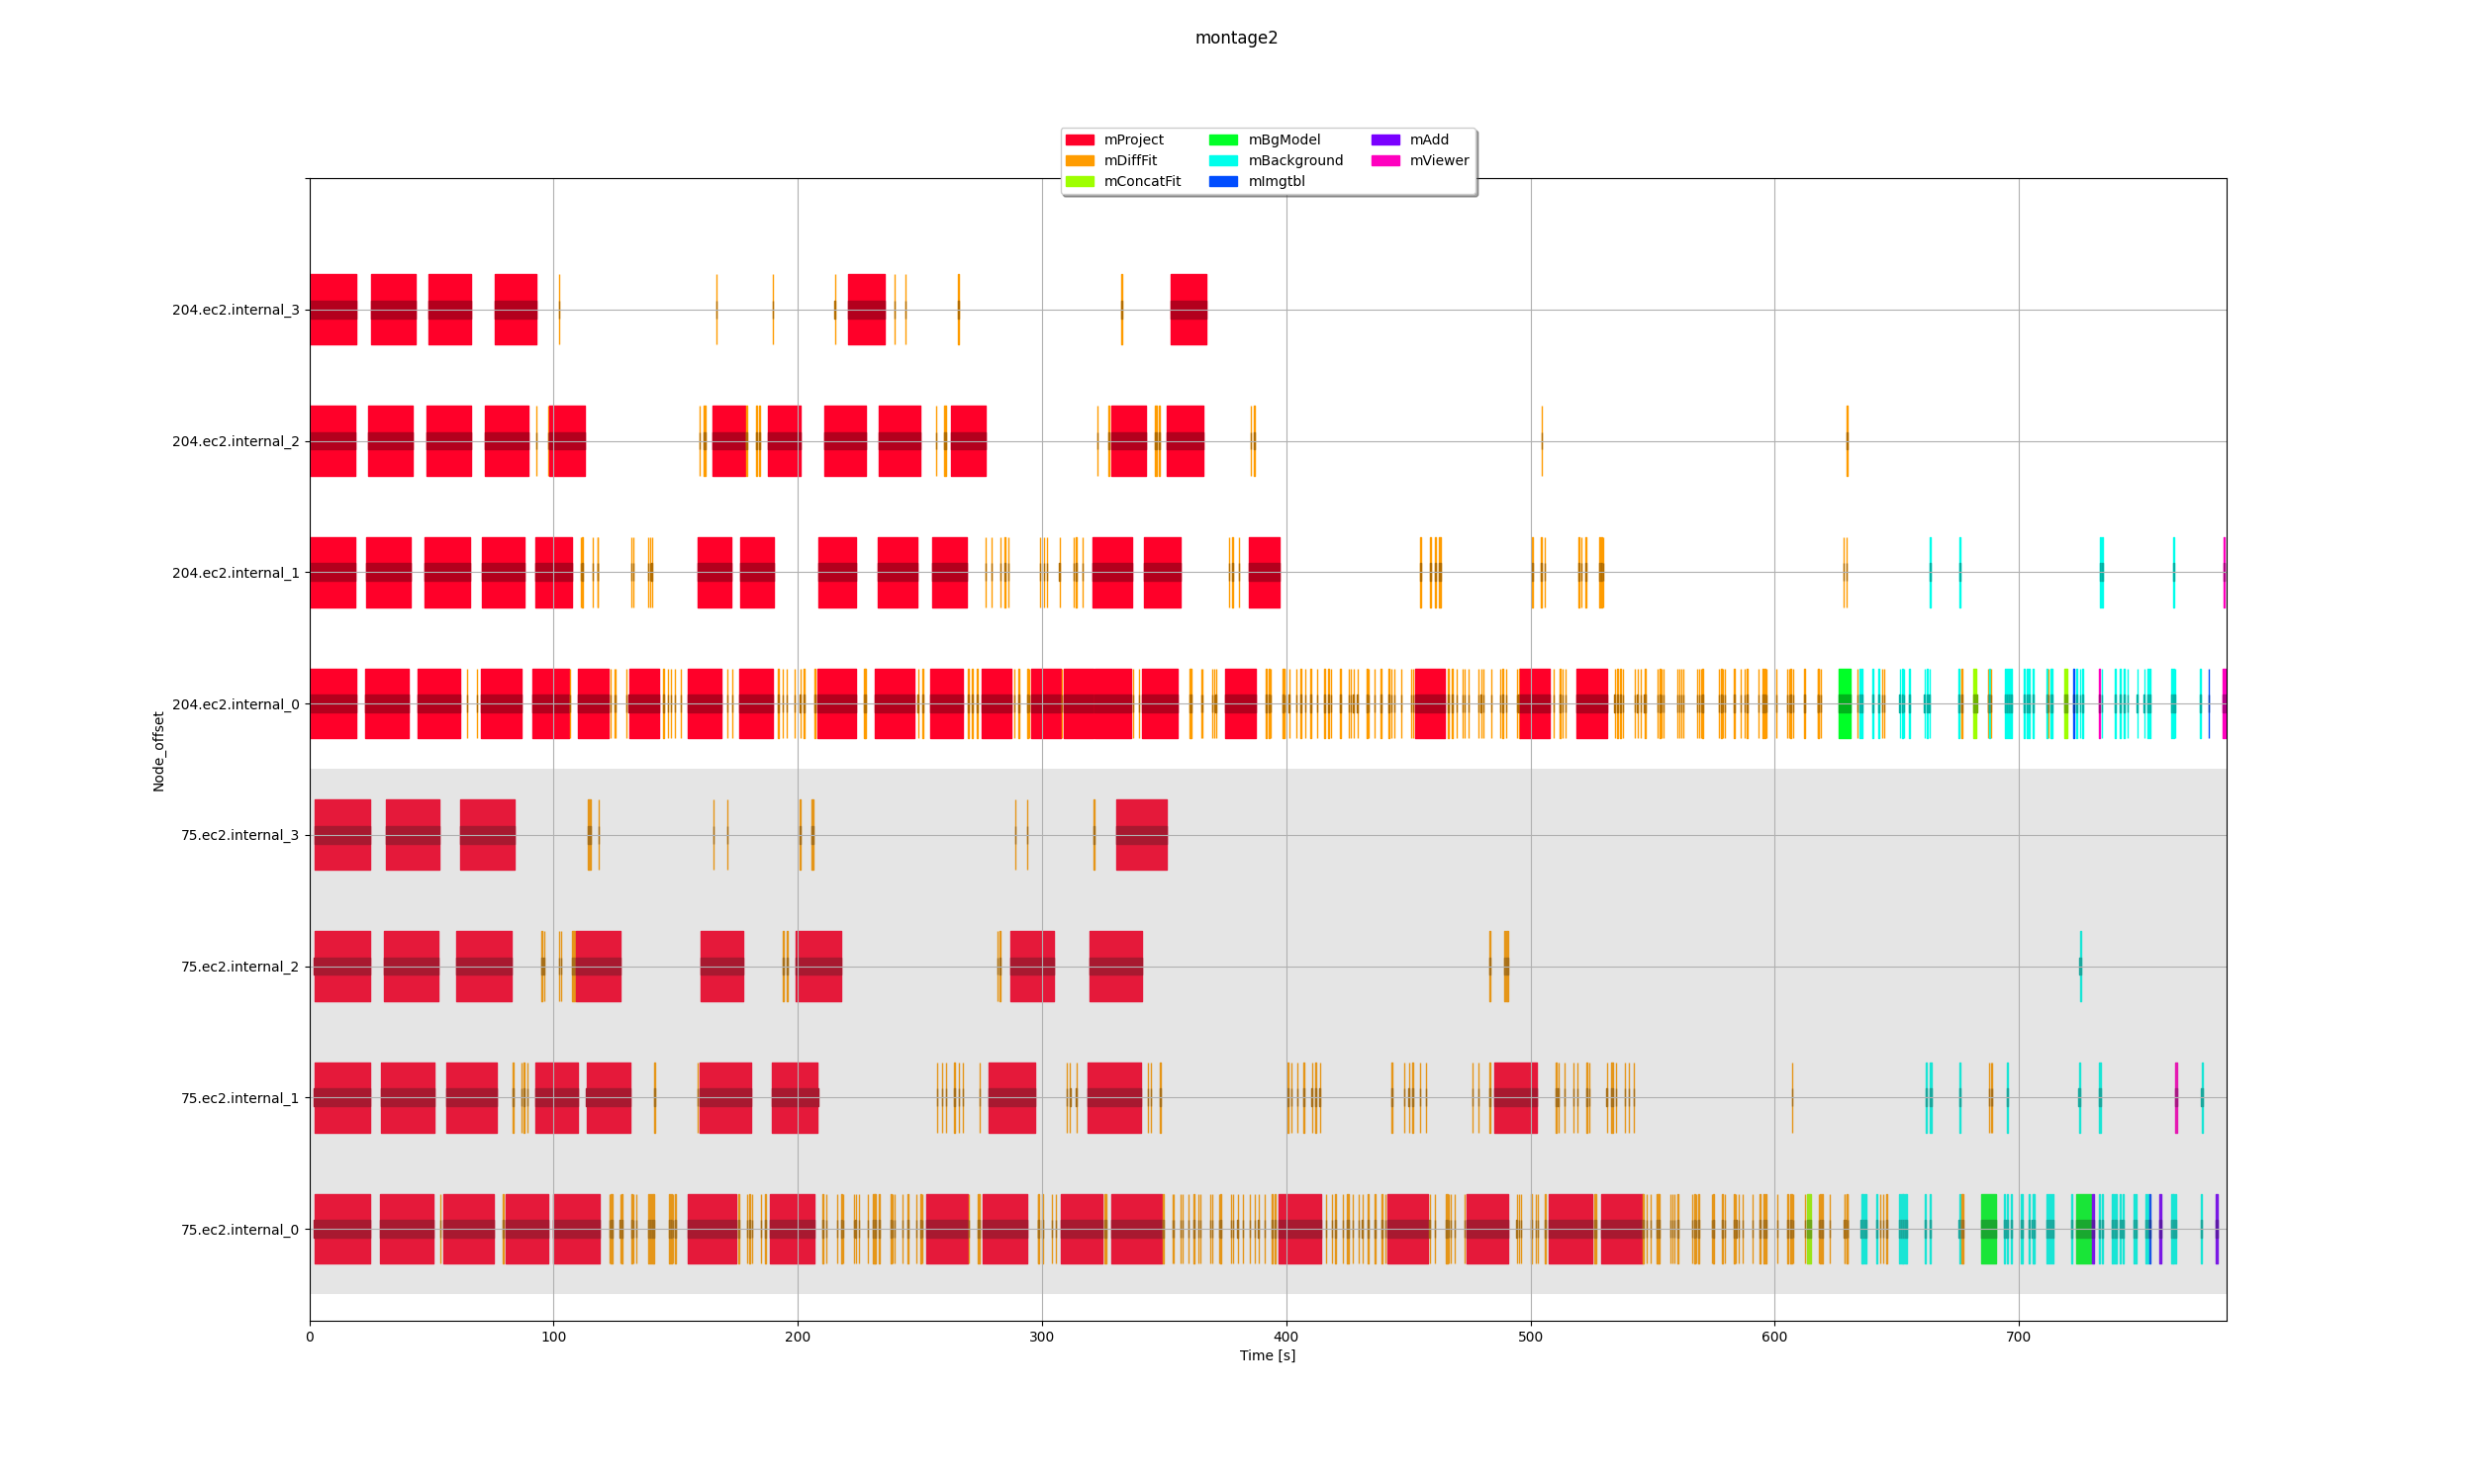
\includegraphics[width=0.75\linewidth]{figures/6-1-m0.25-empty.png}
        \caption[Selected example execution trace for Montage2-v0.25 workflow without static scheduling]{w/o scheduler plugin}
        \label{fig:evaluation:sched:m025:em}
    \end{subfigure}
%%
    \begin{subfigure}{1\textwidth}
        \centering
        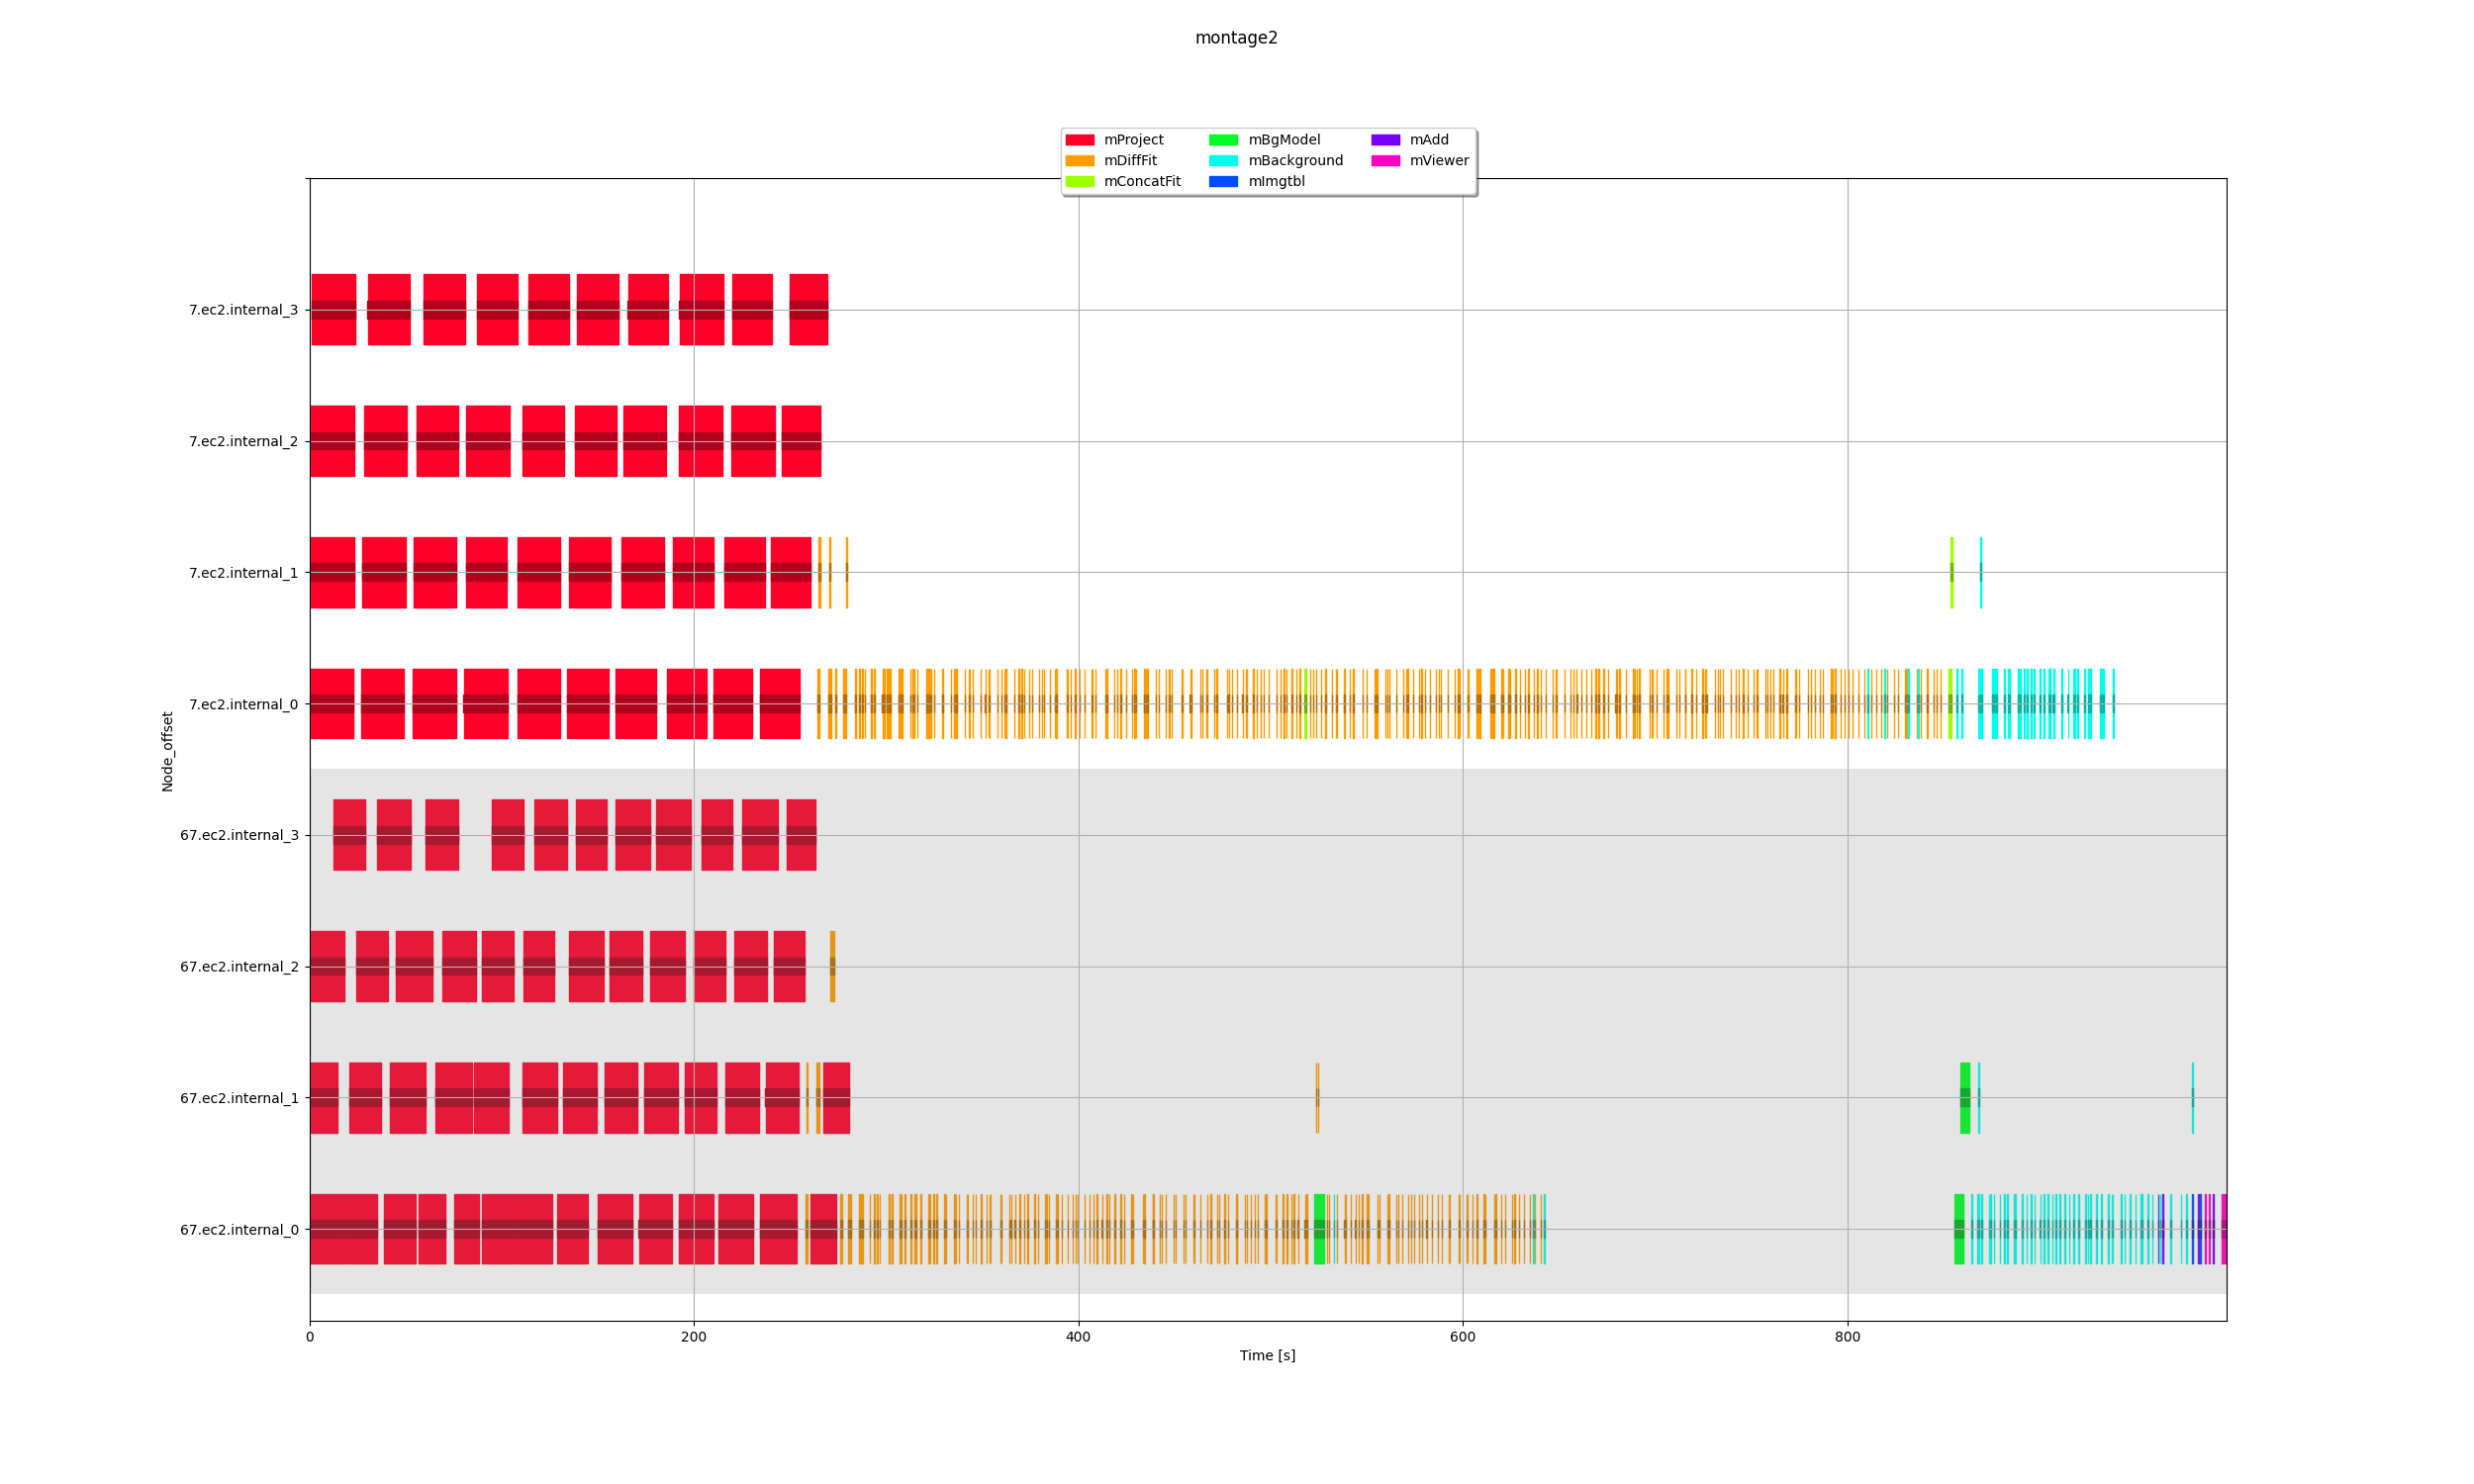
\includegraphics[width=0.75\linewidth]{figures/6-1-m0.25-heft.png}
        \caption[Selected example execution traces for Montage2-v0.25 workflow with HEFT]{HEFT}
        \label{fig:evaluation:sched:m025:heft}
    \end{subfigure}
%%
    \begin{subfigure}{1\textwidth}
        \centering
        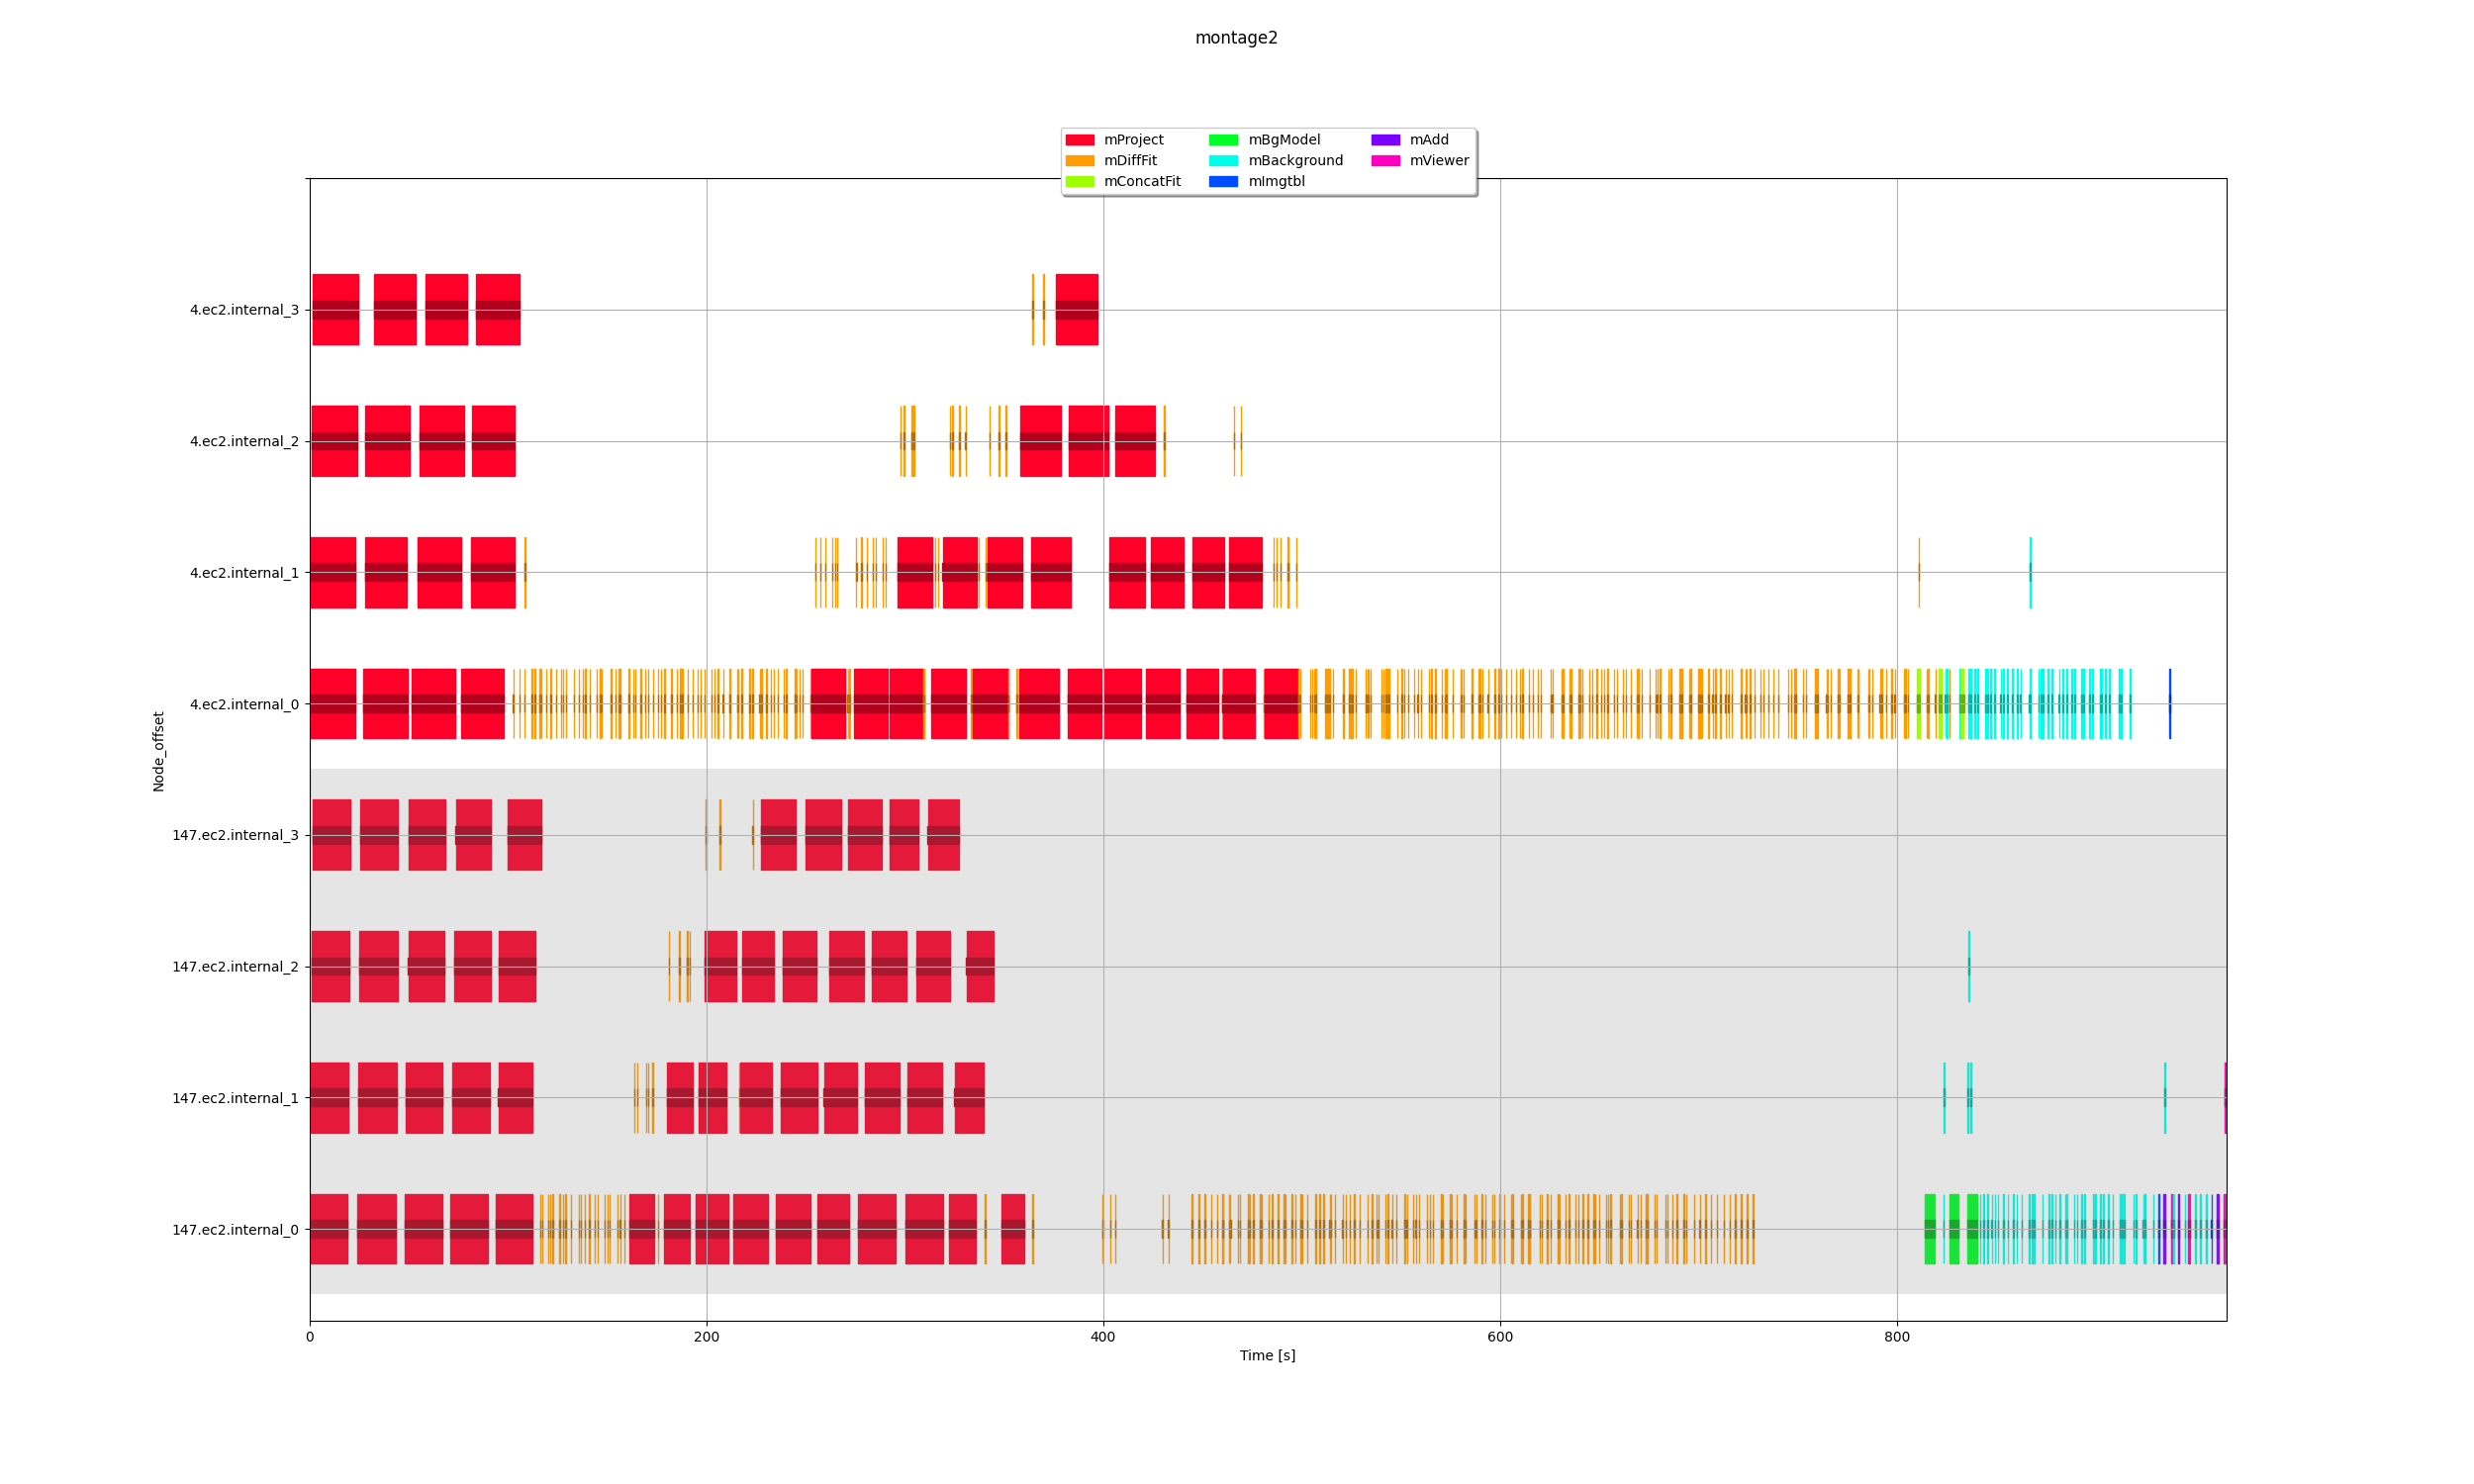
\includegraphics[width=0.75\linewidth]{figures/6-1-m0.25-peft.png}
        \caption[Selected example execution traces for Montage2-v0.25 workflow with PEFT]{PEFT}
        \label{fig:evaluation:sched:m025:peft}
    \end{subfigure}
%%
    \centering
%%
    \caption[Selected example execution traces for Montage2-v0.25 workflow]{Selected example execution traces for Montage2-v0.25.}
%%
    \label{fig:evaluation:sched:m025:plugin}
\end{figure} %%%%%%%
\noindent
Following the trace of the default solution, the longer tasks (\emph{mProject}) are more scattered in time, lessening the load on the Kubernetes components and allowing for a slightly better workload distribution across available computing units.
The same reasoning could also apply to the PEFT execution analysis, however, the \emph{mProject} tasks have still been packed together relatively tight in a schedule, and have not been interjected between \emph{mDiffFit} tasks to such an extent as in the default solution.
Regarding HEFT schedules for Montage workflow, they seem to prioritize finishing tasks based on the length of the path to the root job.
This way, all \emph{mProject} tasks have been assigned the highest priority and finished before \emph{mDiffFit} ones, which have ended with the lowest possible effective task parallelization.



%%%%%%%
\subsection{Scheduling with task clustering}\label{s:Evaluation:Agglomeration}

One way to mitigate the issue of executing multiple short containerized tasks is to introduce task clustering (see section \ref{s:ProblemDomain:TaskClustering}).
The goal of this scenario is to compare the default task clustering solution with the one proposed in this work (section \ref{s:SchedHyperflow:Agglomeration}).

Regarding the workflows considered for this scenario, only Montage workflows are included -- Montage2-v0.25 and Montage2-v1.0 (4846 tasks).
The SoyKB application is relatively small in terms of job count and consists of long-running tasks, thus grouping them further would be of negligible benefit.

To enable task clustering for the default solution, the job agglomeration setup has been configured based on the exemplary configuration\footnotemark[1] in Hyperflow.
Contents of this configuration are presented in listing \ref{lst:task-cluster:montage-config}.
It introduces the buffer setup for selected task operations that are considered clusterable.
The buffering behaviour has been described in section \ref{s:ProblemDomain:Hyperflow}.


\footnotetext[1]{Montage task agglomeration: \url{https://github.com/hyperflow-wms/hyperflow/wiki/Task-agglomeration}, Access: 2021-06-03}

%%%%%%% Agglo Config 
\numberwithin{lstlisting}{section}
\smallskip
\begin{center}
\begin{minipage}{0.6\textwidth}
\lstset{
    string=[s]{"}{"},
    stringstyle=\color{blue},
    comment=[l]{:},
    commentstyle=\color{black},
}
\centering
\begin{lstlisting}[basicstyle=\fontsize{9}{10}\selectfont]
[{
    "matchTask": ["mProject"],
    "size": 2,
    "timeoutMs": 3000
 },
 {
    "matchTask": ["mDiffFit"],
    "size": 6,
    "timeoutMs": 3000
 },
 {
    "matchTask": ["mBackground"],
    "size": 3,
    "timeoutMs": 3000
}]
\end{lstlisting}
\captionof{lstlisting}{Montage task clustering configuration}
\label{lst:task-cluster:montage-config}
\end{minipage}
\end{center}
%%%%%%%



With this configuration, the experiment has been conducted on the smaller Montage2-v0.25 workflow providing the results presented in \cref{tab:metrics-clustering-m025}.
Both solutions with static scheduling proved to be more efficient, achieving roughly 8\% makespan reduction with HEFT and 10\% with PEFT, over the default one with a sole kube-scheduler.
Another benefit of a two-step scheduling is the reduced containerization overhead.
The effectiveness in this aspect is increased by over 400\%.

The HEFT schedule seems to perform the best in terms of grouping the tasks into the least number of containers.
Its behaviour seems to follow the one observed in the scenario without task clustering, however, this time it helps with the reduction of CO, which helps with shortening workflow execution times.
Regarding PEFT solution, it still allows better buffering capabilities for job agglomeration compared to the default one.
Although CO is not as low as the one achieved with HEFT, the computed schedule is even more effective, which is probably a result of introduced \emph{Optimistic Cost Table} adjustments \cite{b:PEFT} as the slowdown is also much lower compared to HEFT case.
All former claims come from an analysis of the execution traces provided in \cref{fig:evaluation:agglo:m025:plugin}.

%%%%
% Tabelka z metrykami - Montage-0.25
\begin{table}[H]
    \centering
    \begin{tabular}{|c|c|c|c|c|}
    \cline{1-5}
        \multirow{2}{*}{Approach} 
        &
        \multicolumn{4}{|c|}{Metrics} \\
    \cline{2-5}
        & Makespan & Slowdown & SLR & CO \\
    \cline{1-5}
        kube-scheduler & 408 & 87 & 11.21 & 1028 \\
    \cline{1-5}
        HEFT + kube-scheduler & 376 & 199 & 11.19 & 187 \\
    \cline{1-5}
        PEFT + kube-scheduler & 365 & 111 & 10.89 & 243 \\
    \cline{1-5}
    \end{tabular}
    \caption{Average metric results of Montage2-v0.25 execution with task clustering}
    \label{tab:metrics-clustering-m025}
\end{table}
%%%%

%%%% Traces - Montage-v0.25
\begin{figure}[H]
\begin{subfigure}{0.75\textwidth}
\centering
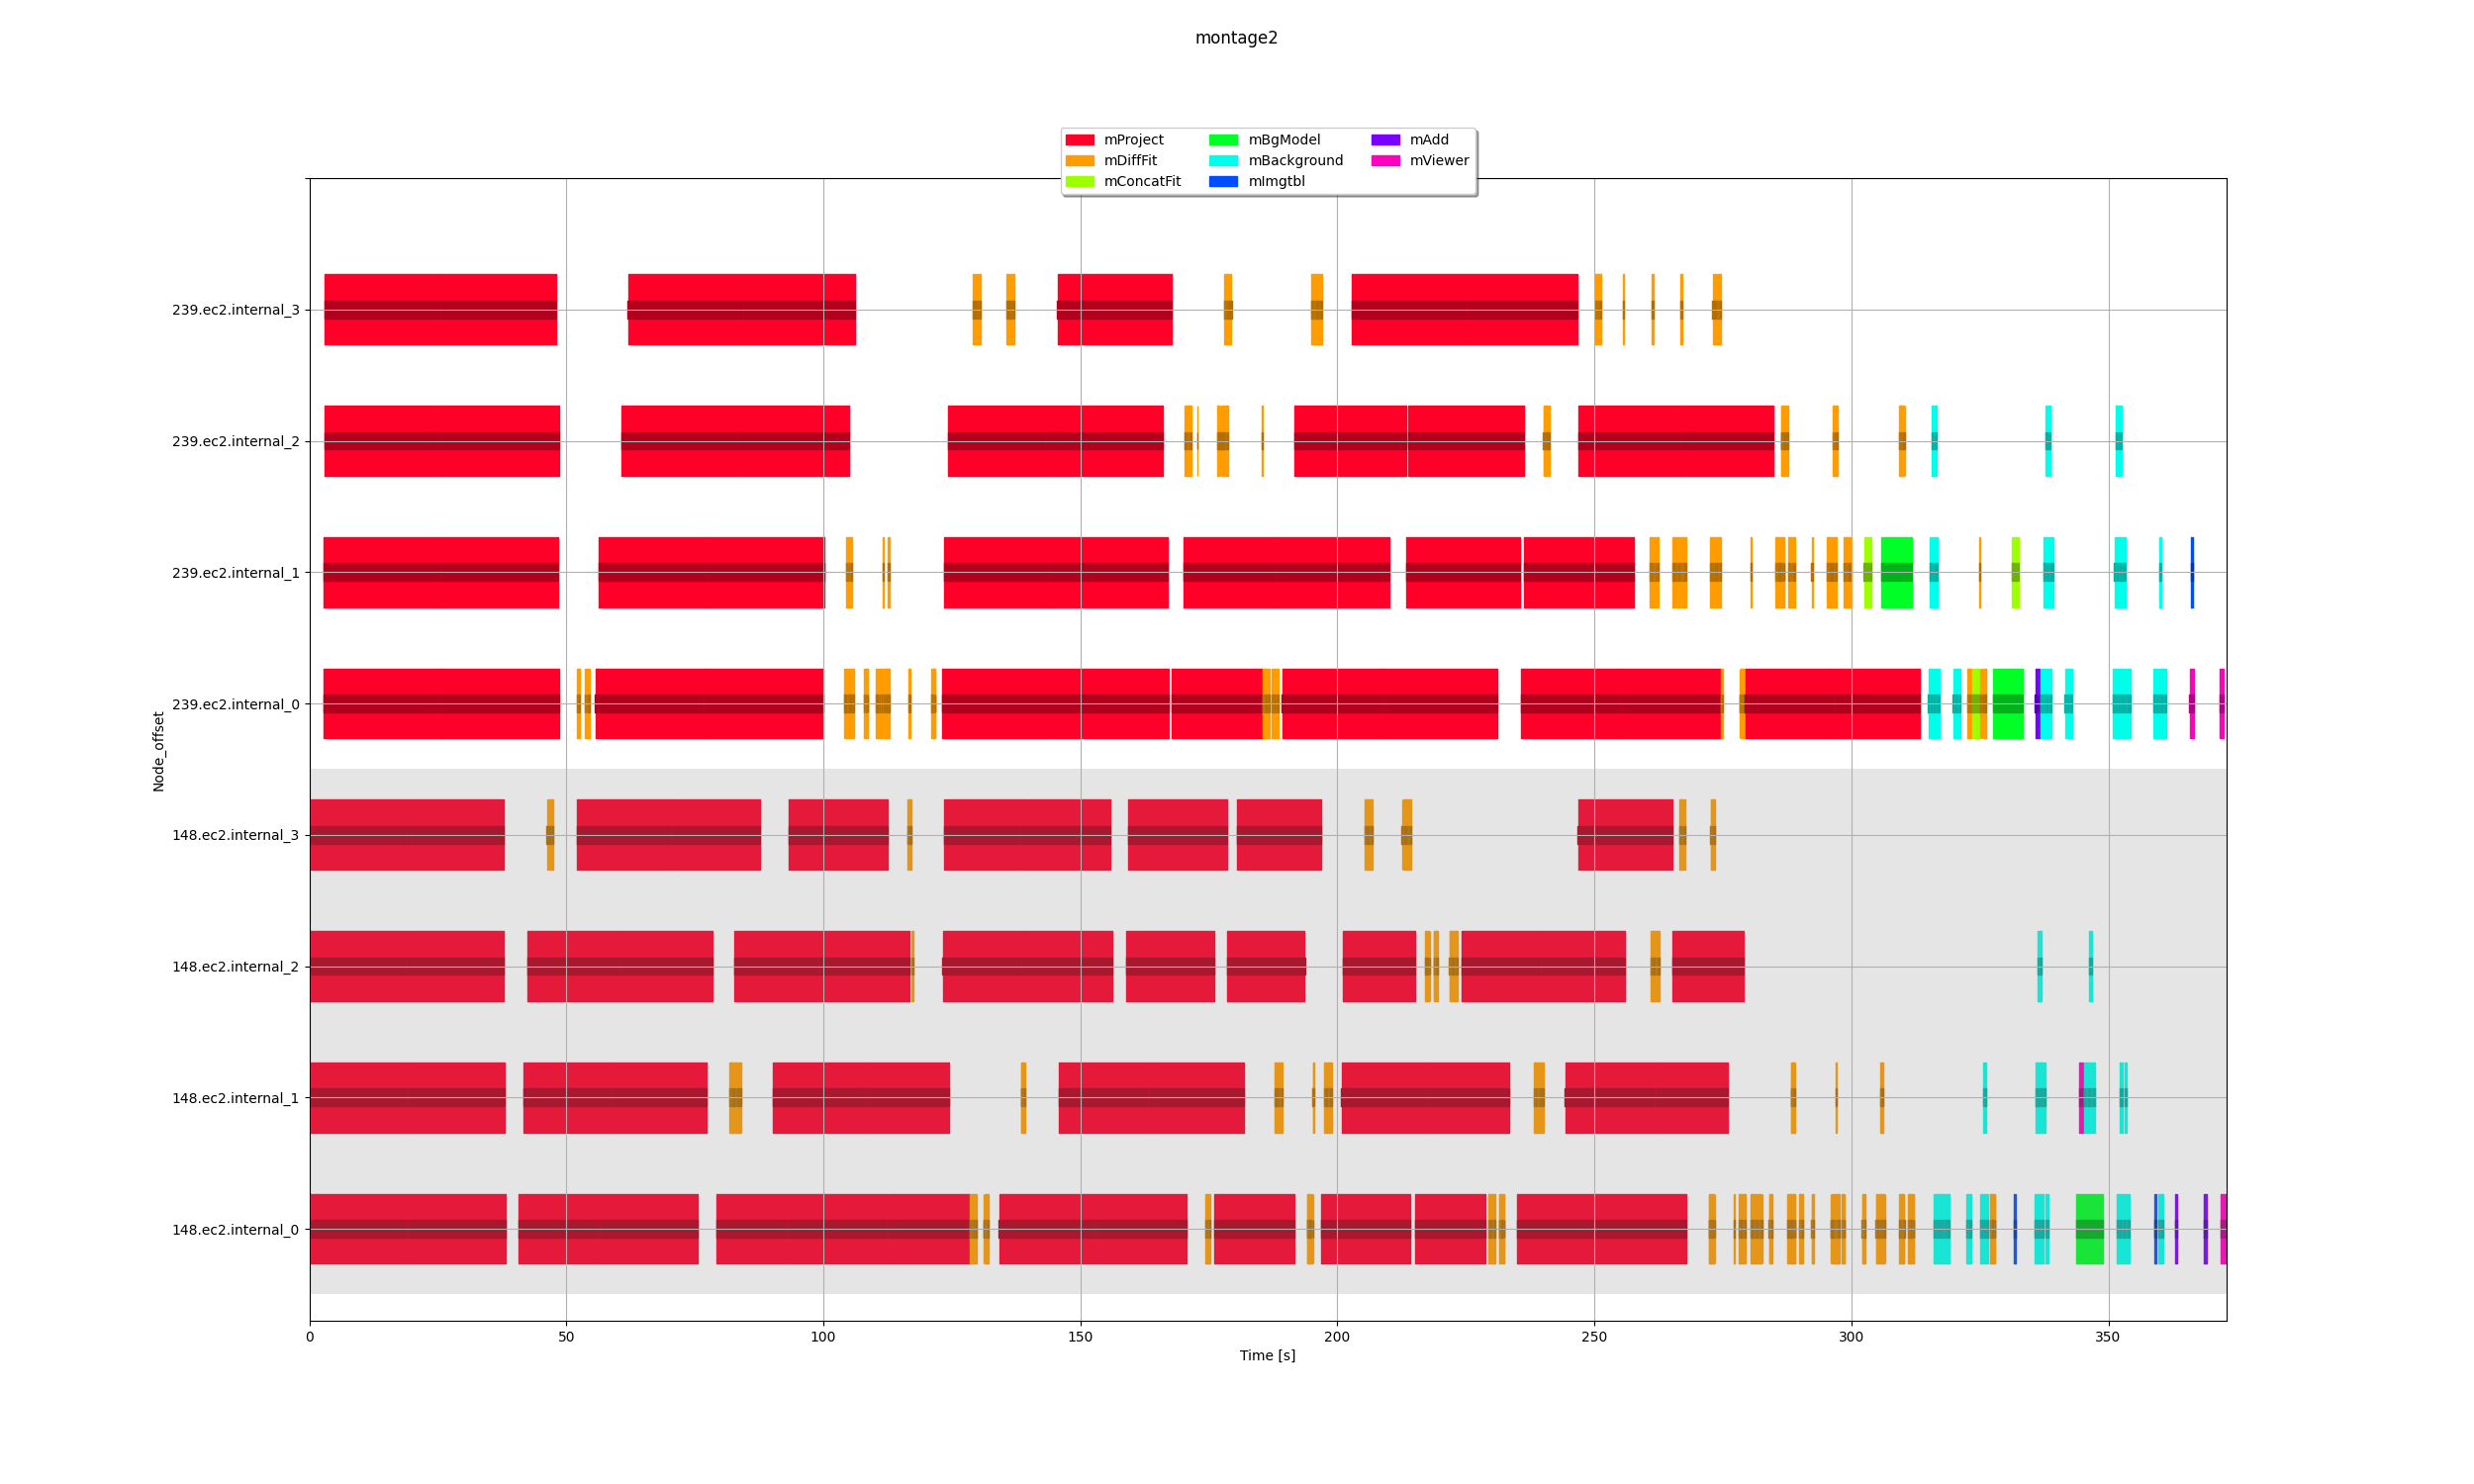
\includegraphics[width=1\linewidth]{figures/6-2-m0.25-agglo-empty.png}
\caption[Selected example execution trace for Montage2-v0.25 workflow with task clustering and no scheduler plugin]{w/o scheduler plugin}
\label{fig:evaluation:agglo:m025:empty}
\end{subfigure}
\begin{subfigure}{0.75\textwidth}
\centering
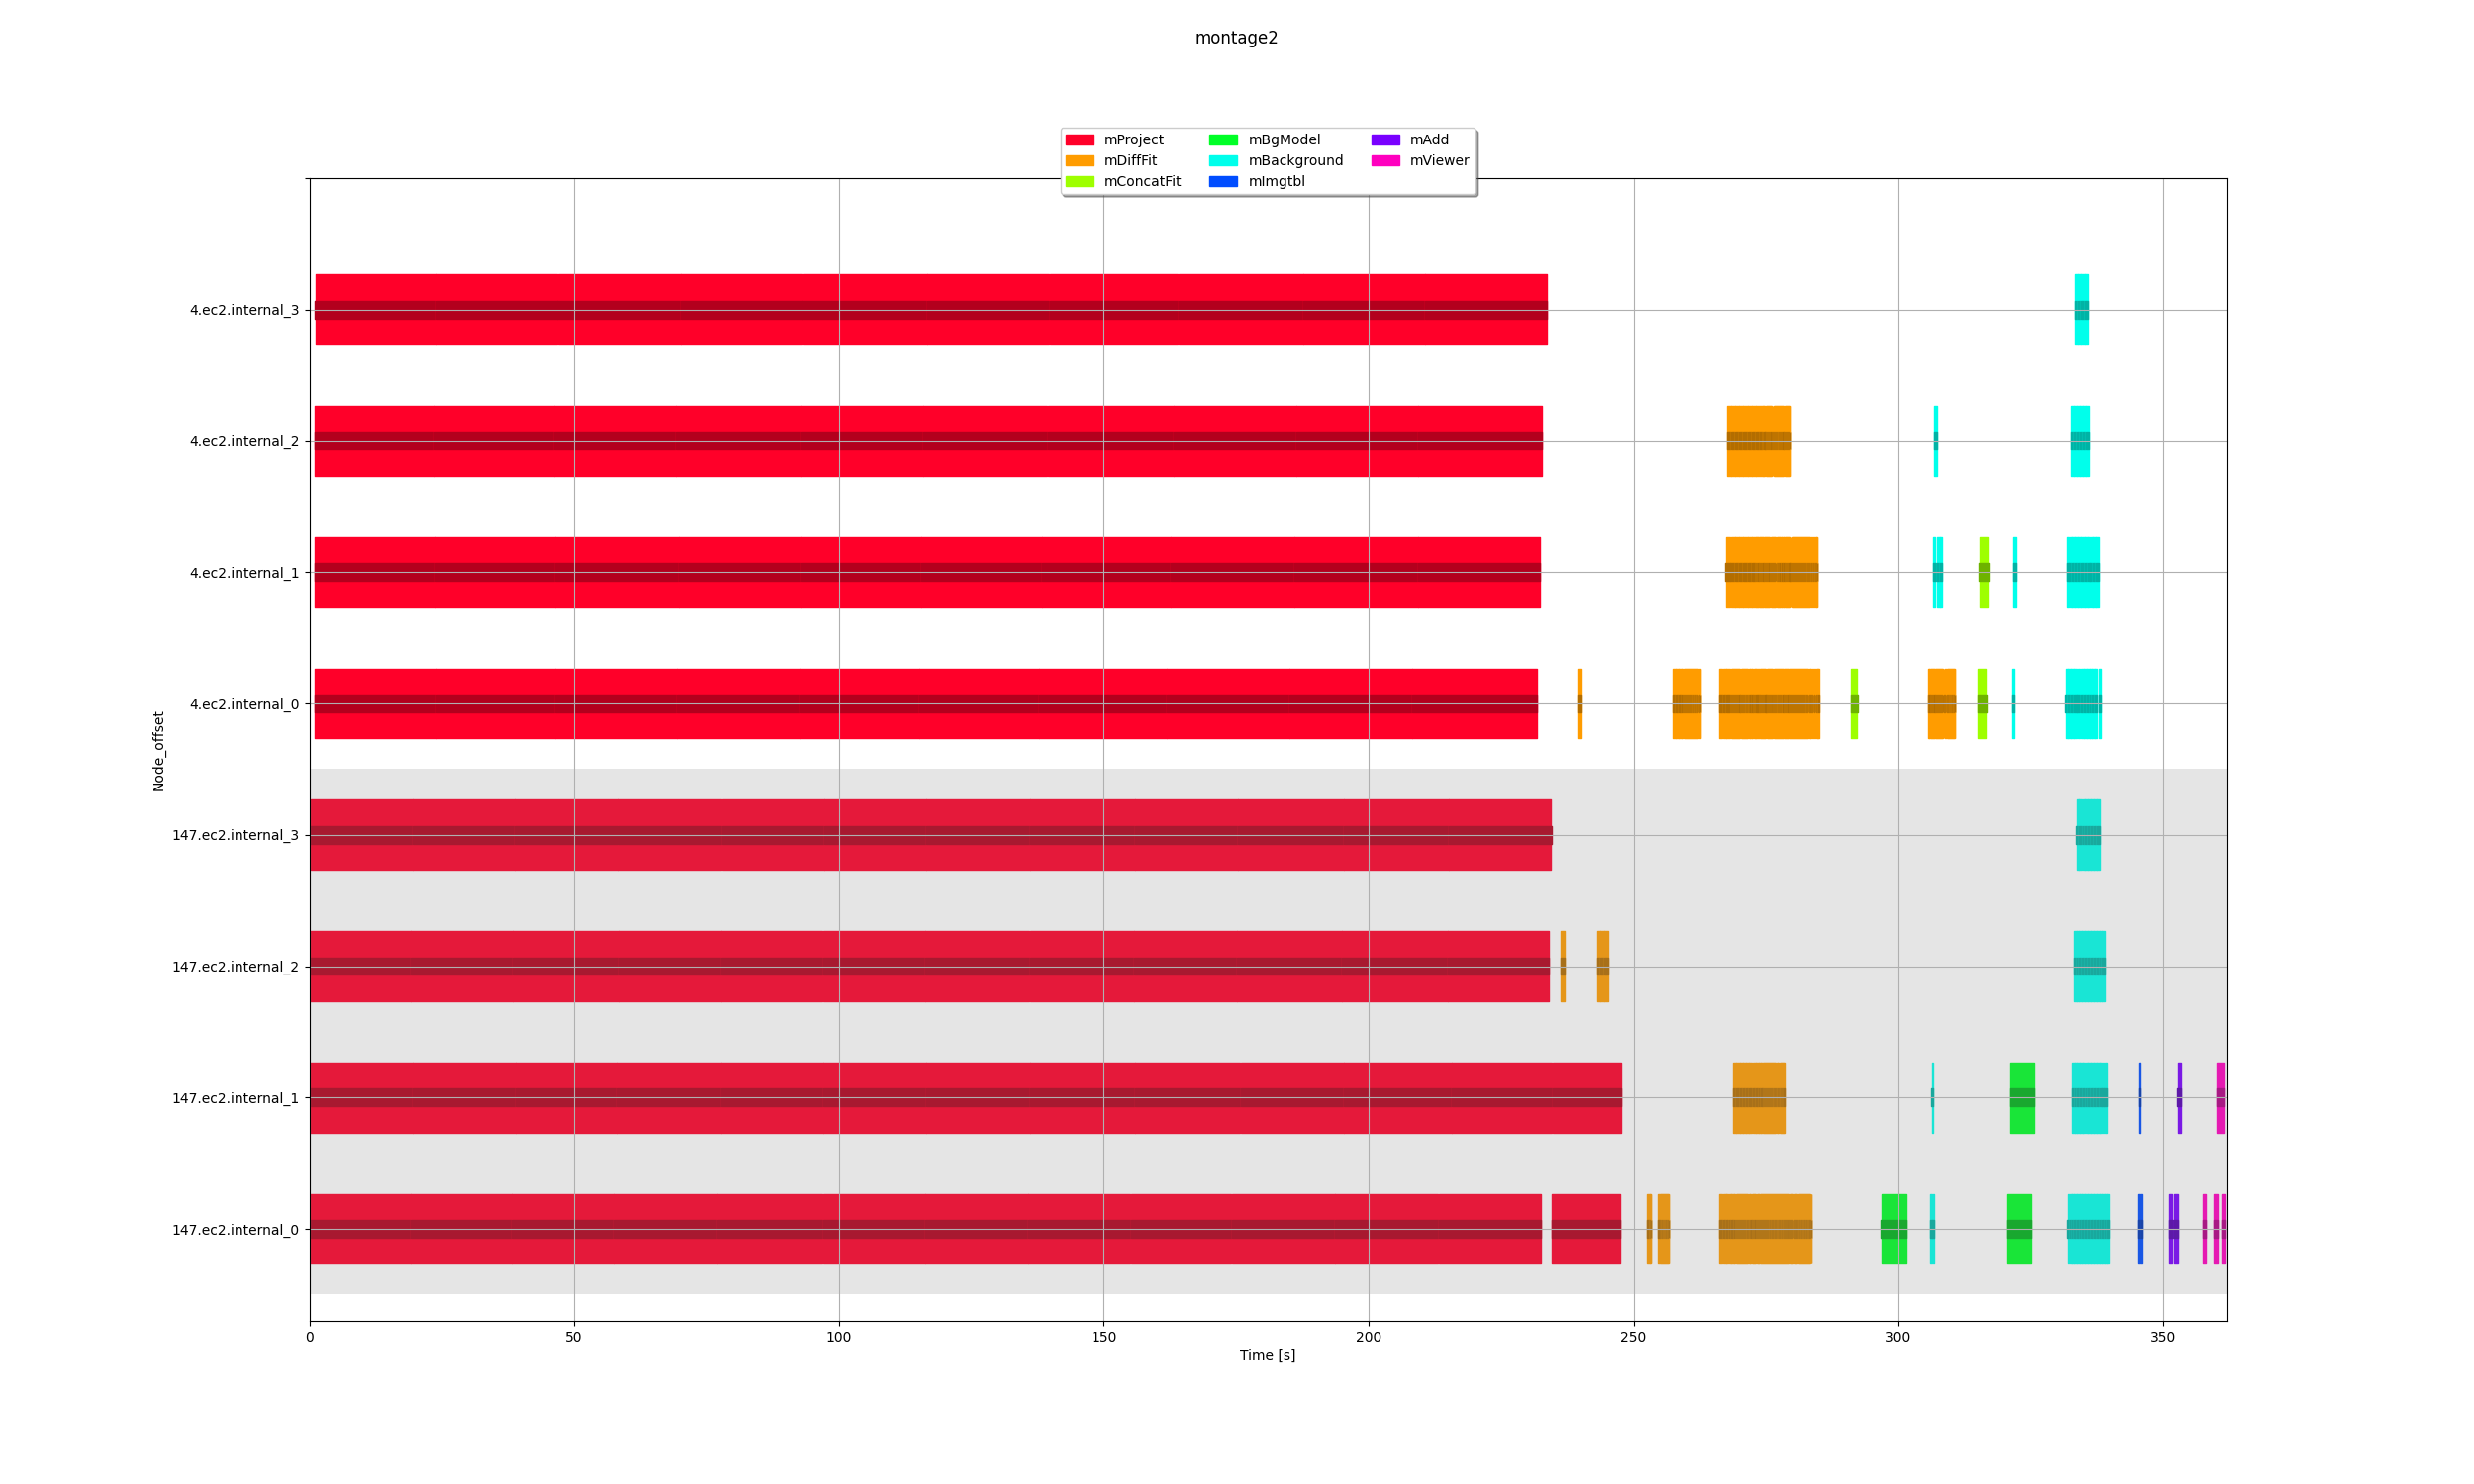
\includegraphics[width=1\linewidth]{figures/6-2-m0.25-agglo-heft.png}
\caption[Selected example execution traces for Montage2-v0.25 workflow with HEFT and task clustering]{HEFT}
\label{fig:evaluation:agglo:m025:heft}
\end{subfigure}
\begin{subfigure}{0.75\textwidth}
\centering
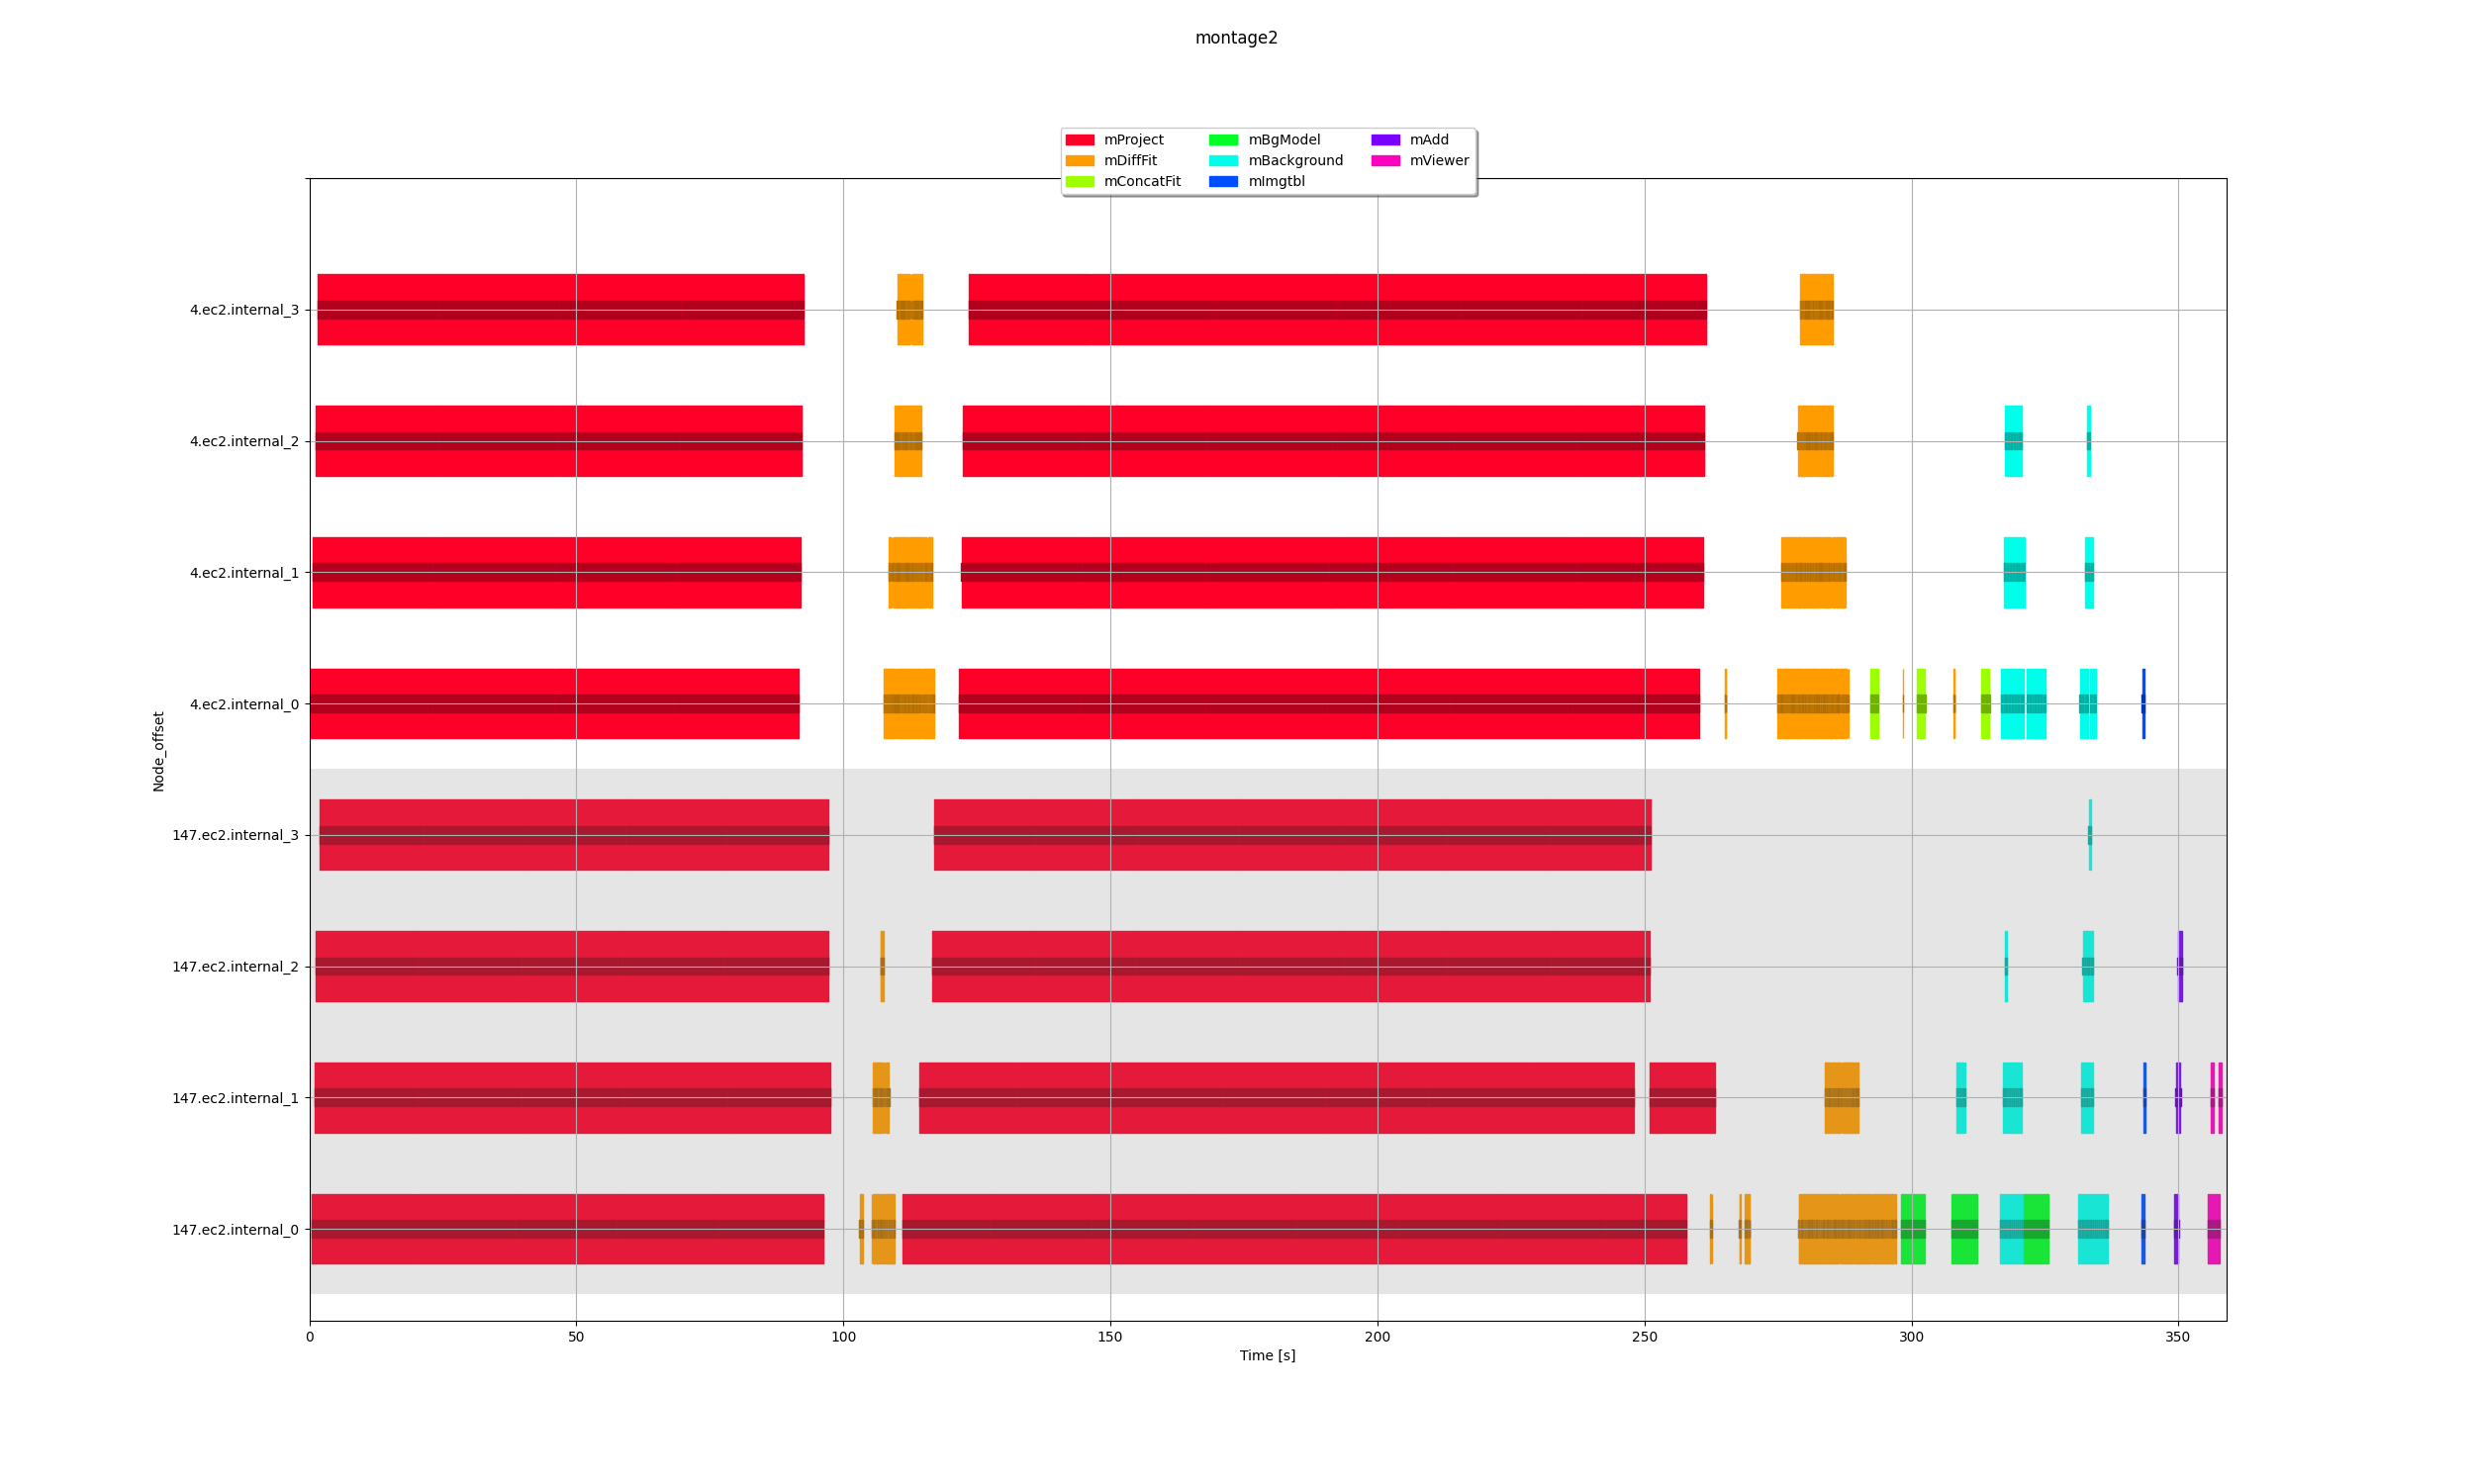
\includegraphics[width=1\linewidth]{figures/6-2-m0.25-agglo-peft.png}
\caption[Selected example execution traces for Montage2-v0.25 workflow with PEFT and task clustering]{PEFT}
\label{fig:evaluation:agglo:m025:peft}
\end{subfigure}
\centering
%%
\caption[Selected example execution traces for Montage2-v0.25 workflow with task clustering]{Selected example execution traces for Montage2-v0.25 workflow with task clustering.}
\label{fig:evaluation:agglo:m025:plugin}
\end{figure}
%%%% KONIEC FIG @@@@@@@@@@@


The two-step scheduling seems to work better for larger workflows as well.
In the case of Montage2-v1.0 workflow, both HEFT and PEFT schedules have proven to be more effective than the default solution, with HEFT shortening the makespan by roughly 8\% and reducing CO by over 80\%, according to the metric values (\cref{tab:metrics-clustering-m10}).
Unexpectedly, the achieved job slowdown for approaches with applied static scheduling is for the first time better than the others.


%%% Tabelka z metrykami - Montage-1.0
\begin{table}[H]
    \centering
    \begin{tabular}{|c|c|c|c|c|}
    \cline{1-5}
        \multirow{2}{*}{Approach} 
        &
        \multicolumn{4}{|c|}{Metrics} \\
    \cline{2-5}
        & Makespan & Job slowdown & SLR & CO \\
    \cline{1-5}
        kube-scheduler & 779 & 537 & 7.6 & 8200 \\
    \cline{1-5}
        HEFT + kube-scheduler & 712 & 239 & 7.1 & 1271 \\
    \cline{1-5}
        PEFT + kube-scheduler & 770 & 256 & 7.3 & 2008 \\
    \cline{1-5}
    \end{tabular}
    \caption{Average metric results of Montage2-v1.0 execution with task clustering}
    \label{tab:metrics-clustering-m10}
\end{table}
%%%

There is no much difference in an execution flow between larger and smaller Montage workflows.
From the \cref{fig:evaluation:agglo:m10:plugin}, it seems that all analyzed approaches follow the already observed behaviour.

Looking at the results, running a lower number of containers, but with a longer lifespan, has been proven to positively impact the overall workflow execution performance, no matter which application is run.
The other valuable conclusion of the provided analysis is that larger workflows have their possible makespan reduction highly reliant on lowering container overhead times, while the smaller ones are slightly more schedule sensitive.

Lastly, it is worth mentioning that with task clustering, the problem of low workload parallelization, observed during the experiment without agglomeration, has been resolved.
Grouping tasks into containerized jobs prolongs the container lifespan, which makes it easier to distribute the load across the node resources in a Kubernetes cluster.


%%%%%% Traces - Montage-v1.0
\begin{figure}[H]
\begin{subfigure}{0.75\textwidth}
\centering
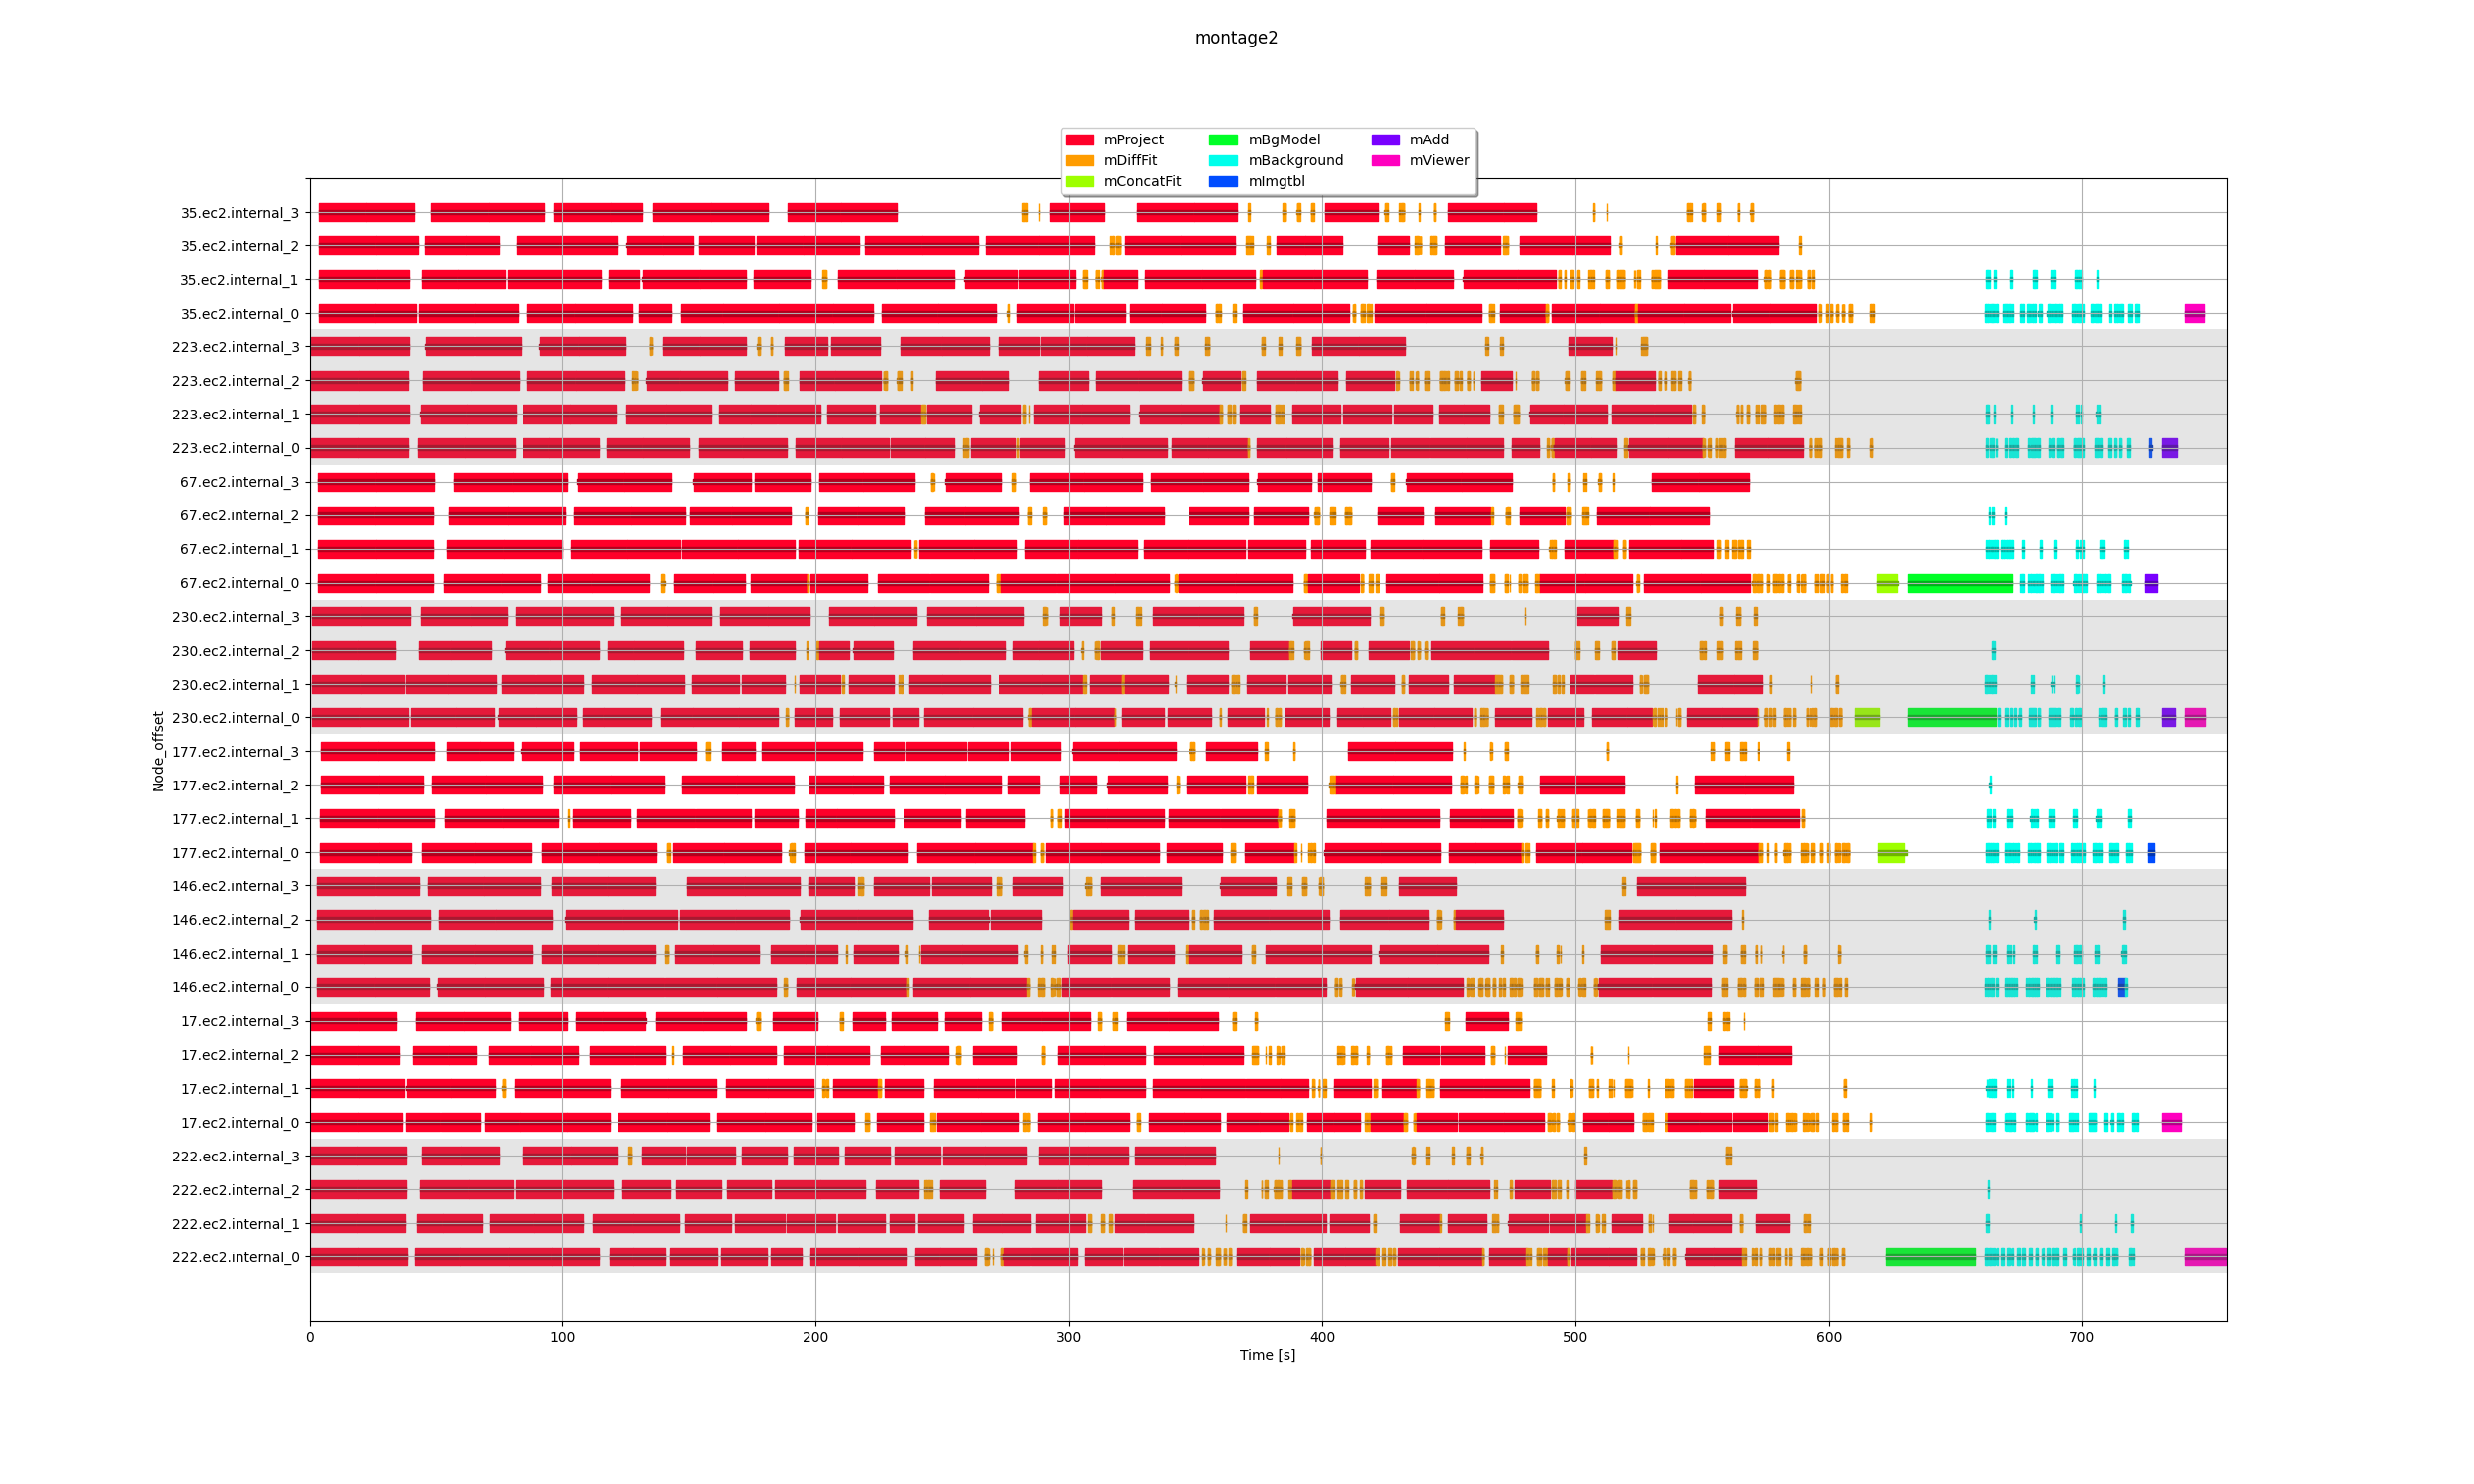
\includegraphics[width=1\linewidth]{figures/6-2-m1.0-agglo-empty.png}
\caption[Selected example execution trace for Montage2-v1.0 workflow with task clustering and no scheduler plugin]{w/o scheduler plugin}
\label{fig:evaluation:agglo:m10:empty}
\end{subfigure}
\begin{subfigure}{0.75\textwidth}
\centering
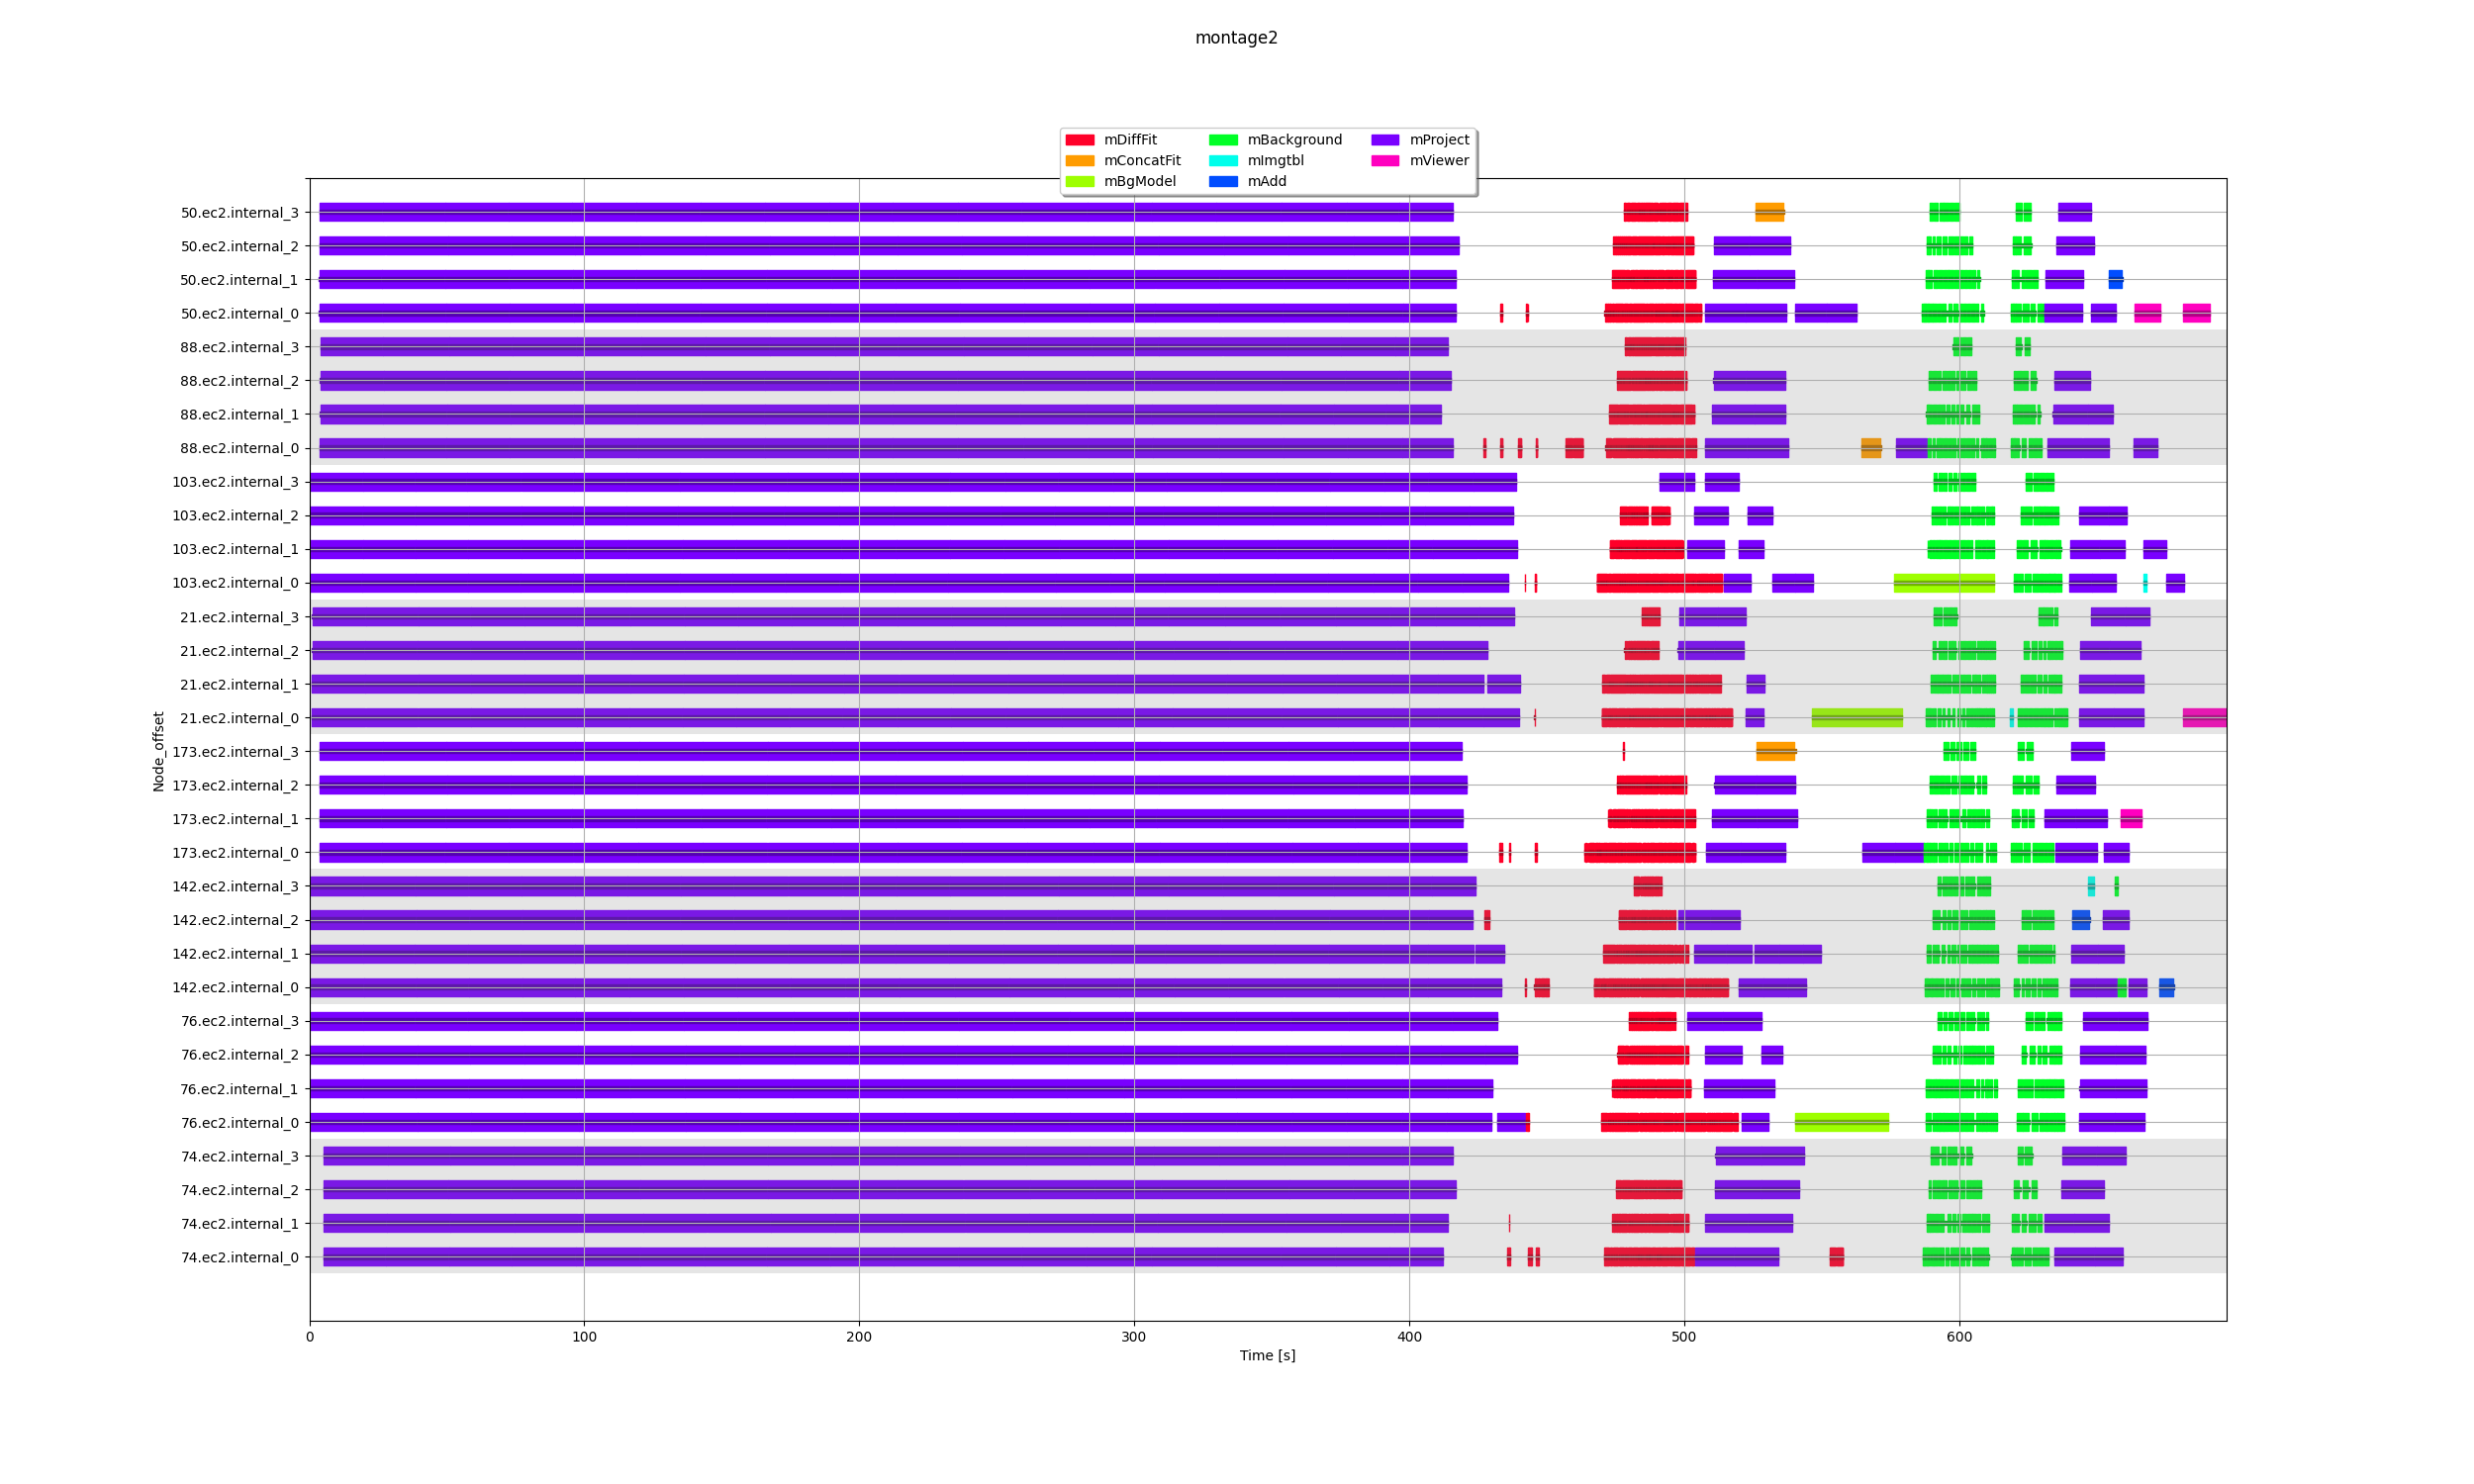
\includegraphics[width=1\linewidth]{figures/6-2-m1.0-agglo-heft.png}
\caption[Selected example execution traces for Montage2-v1.0 workflow with HEFT and task clustering]{HEFT}
\label{fig:evaluation:agglo:m10:heft}
\end{subfigure}
\begin{subfigure}{0.75\textwidth}
\centering
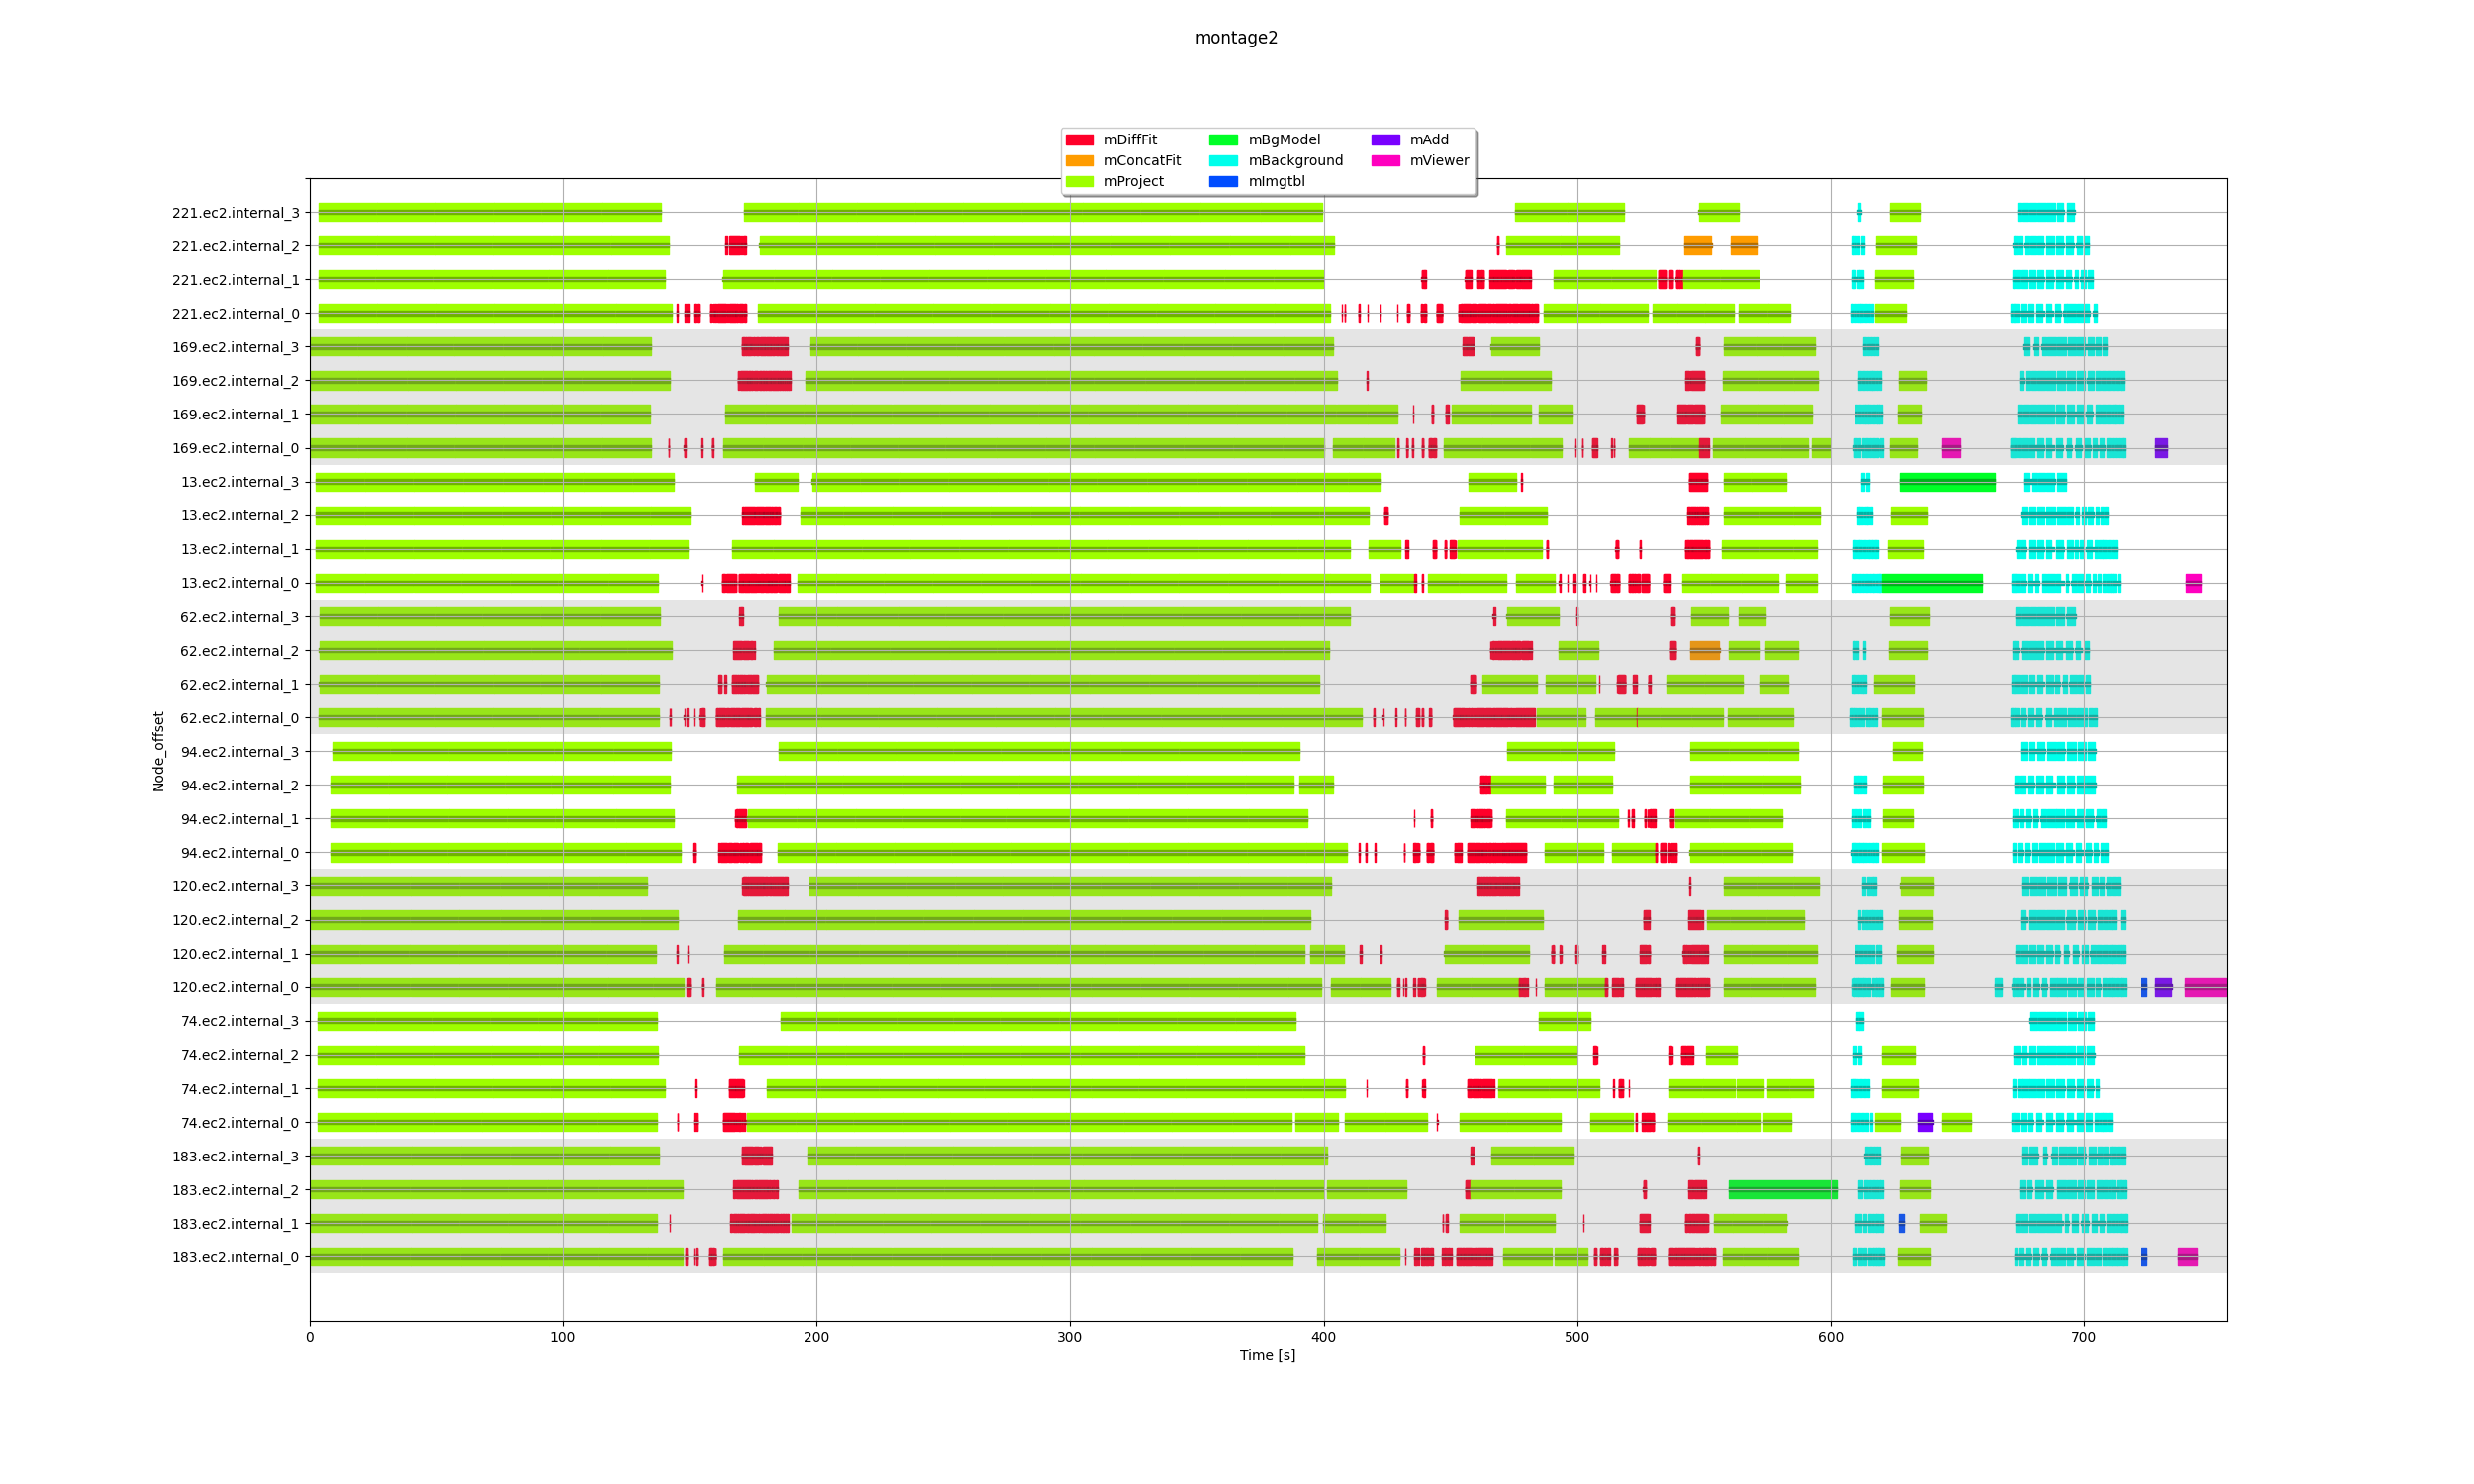
\includegraphics[width=1\linewidth]{figures/6-2-m1.0-agglo-peft.png}
\caption[Selected example execution traces for Montage2-v1.0 workflow with PEFT and task clustering]{PEFT}
\label{fig:evaluation:agglo:m10:peft}
\end{subfigure}
\centering
%%
\caption[Selected example execution traces for Montage2-v1.0 workflow with task clustering]{Selected example execution traces for Montage2-v1.0 workflow with task clustering.}
\label{fig:evaluation:agglo:m10:plugin}
\end{figure}
%%%%%% 


%%%%
% \begin{figure}[H]
% \centering
% 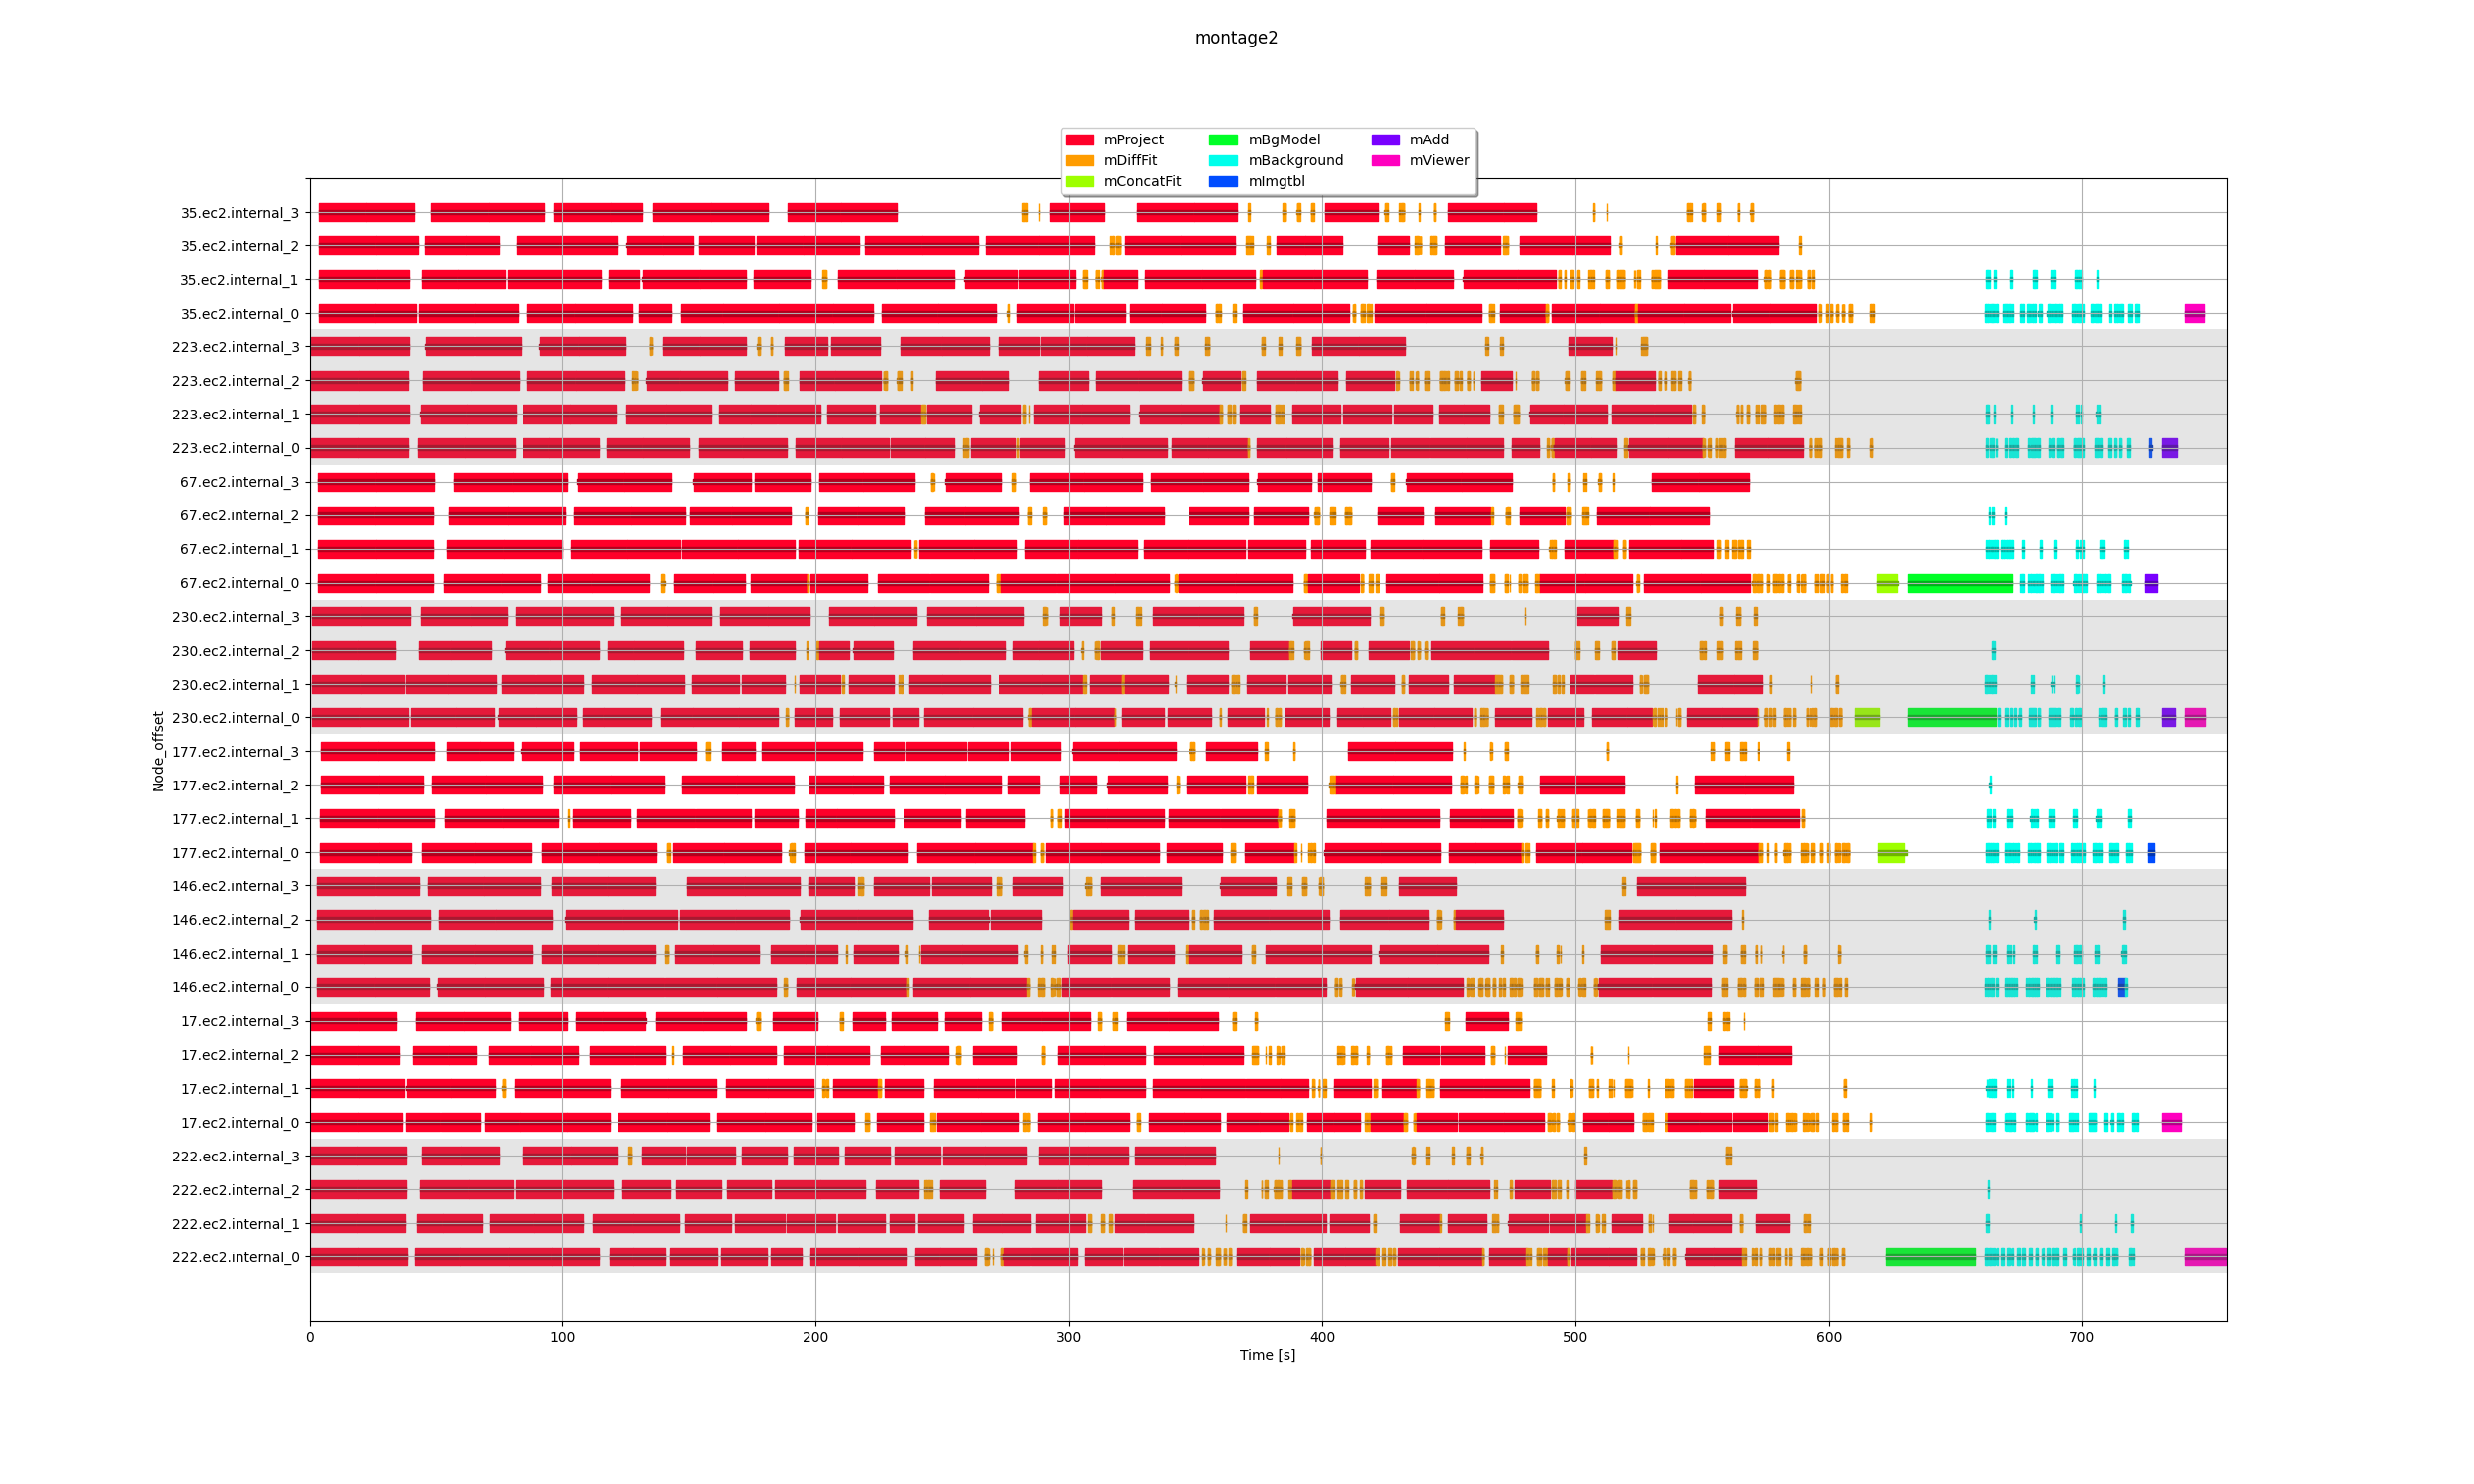
\includegraphics[width=1\linewidth]{figures/6-2-m1.0-agglo-empty.png}
% \caption[Task clustering without workflow scheduling - Montage-1.0]{Task clustering without workflow scheduling - Montage-1.0.}
% \label{fig:evaluation:agglo:m10:empty}
% \end{figure}

% \begin{figure}[H]
% \centering
% 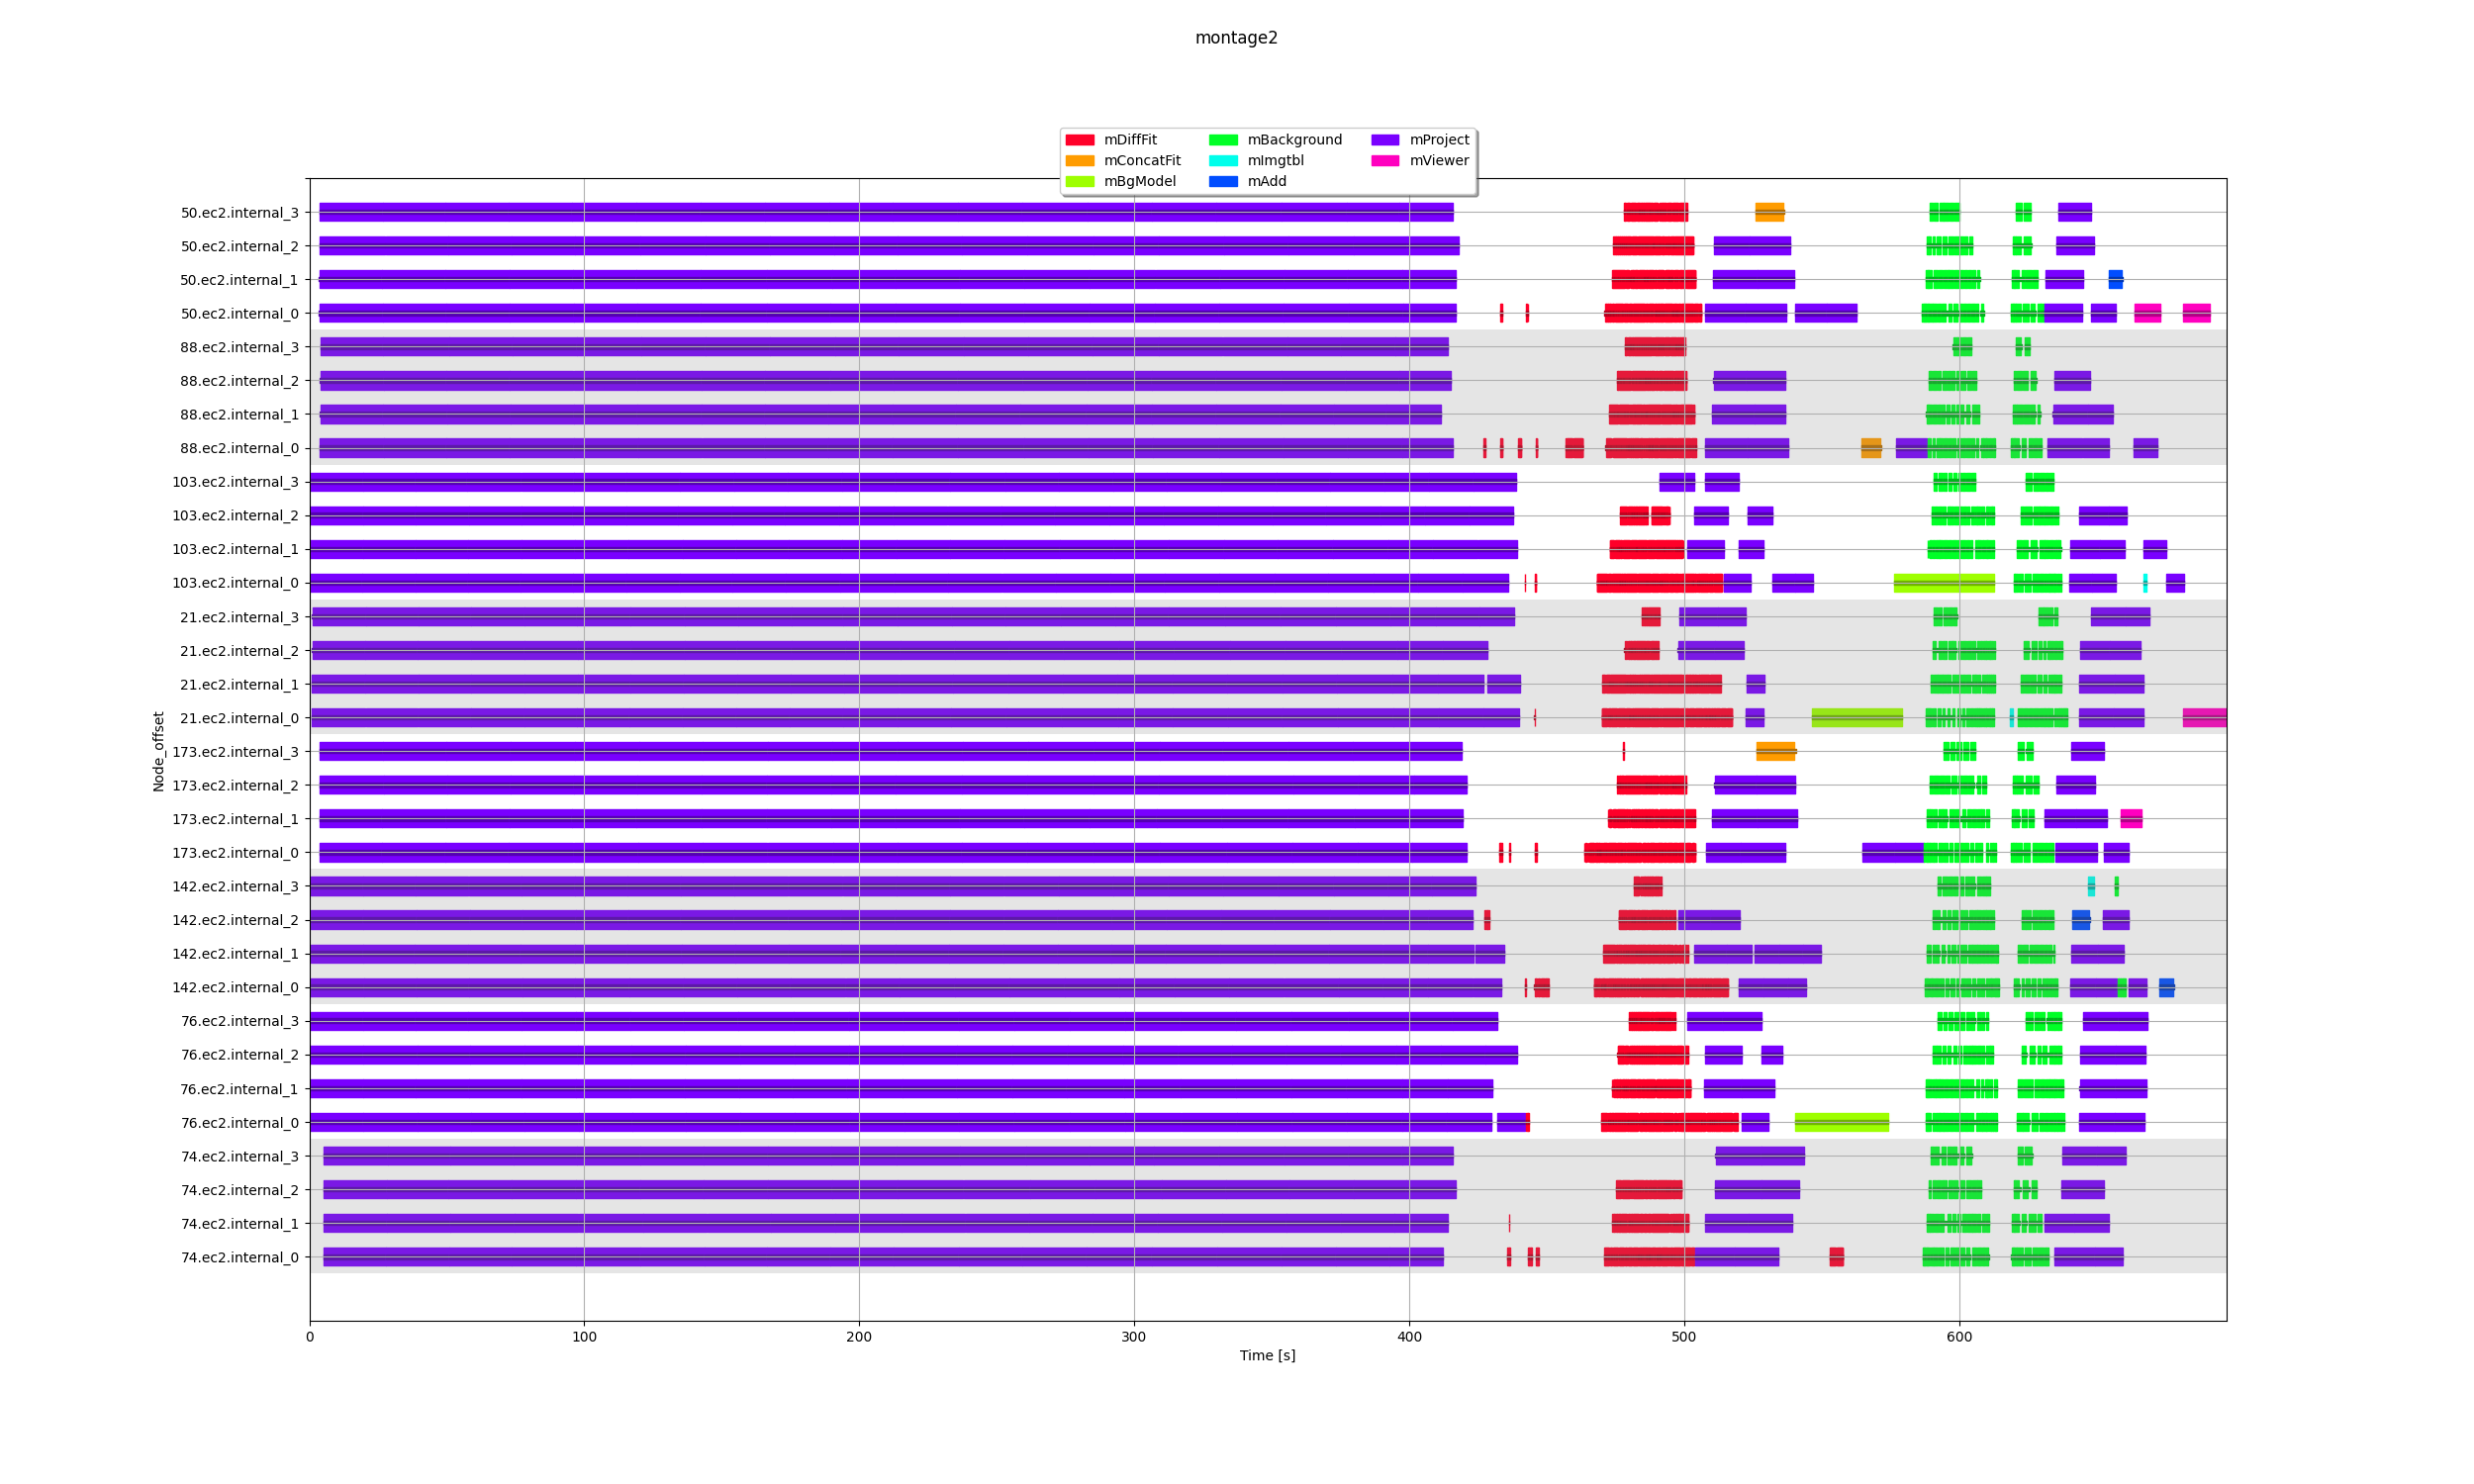
\includegraphics[width=1\linewidth]{figures/6-2-m1.0-agglo-heft.png}
% \caption[Task clustering on HEFT-planned schedule - Montage-1.0]{Task clustering on HEFT-planned schedule - Montage-0.25.}
% \label{fig:evaluation:agglo:m10:heft}
% \end{figure}

% \begin{figure}[H]
% \centering
% 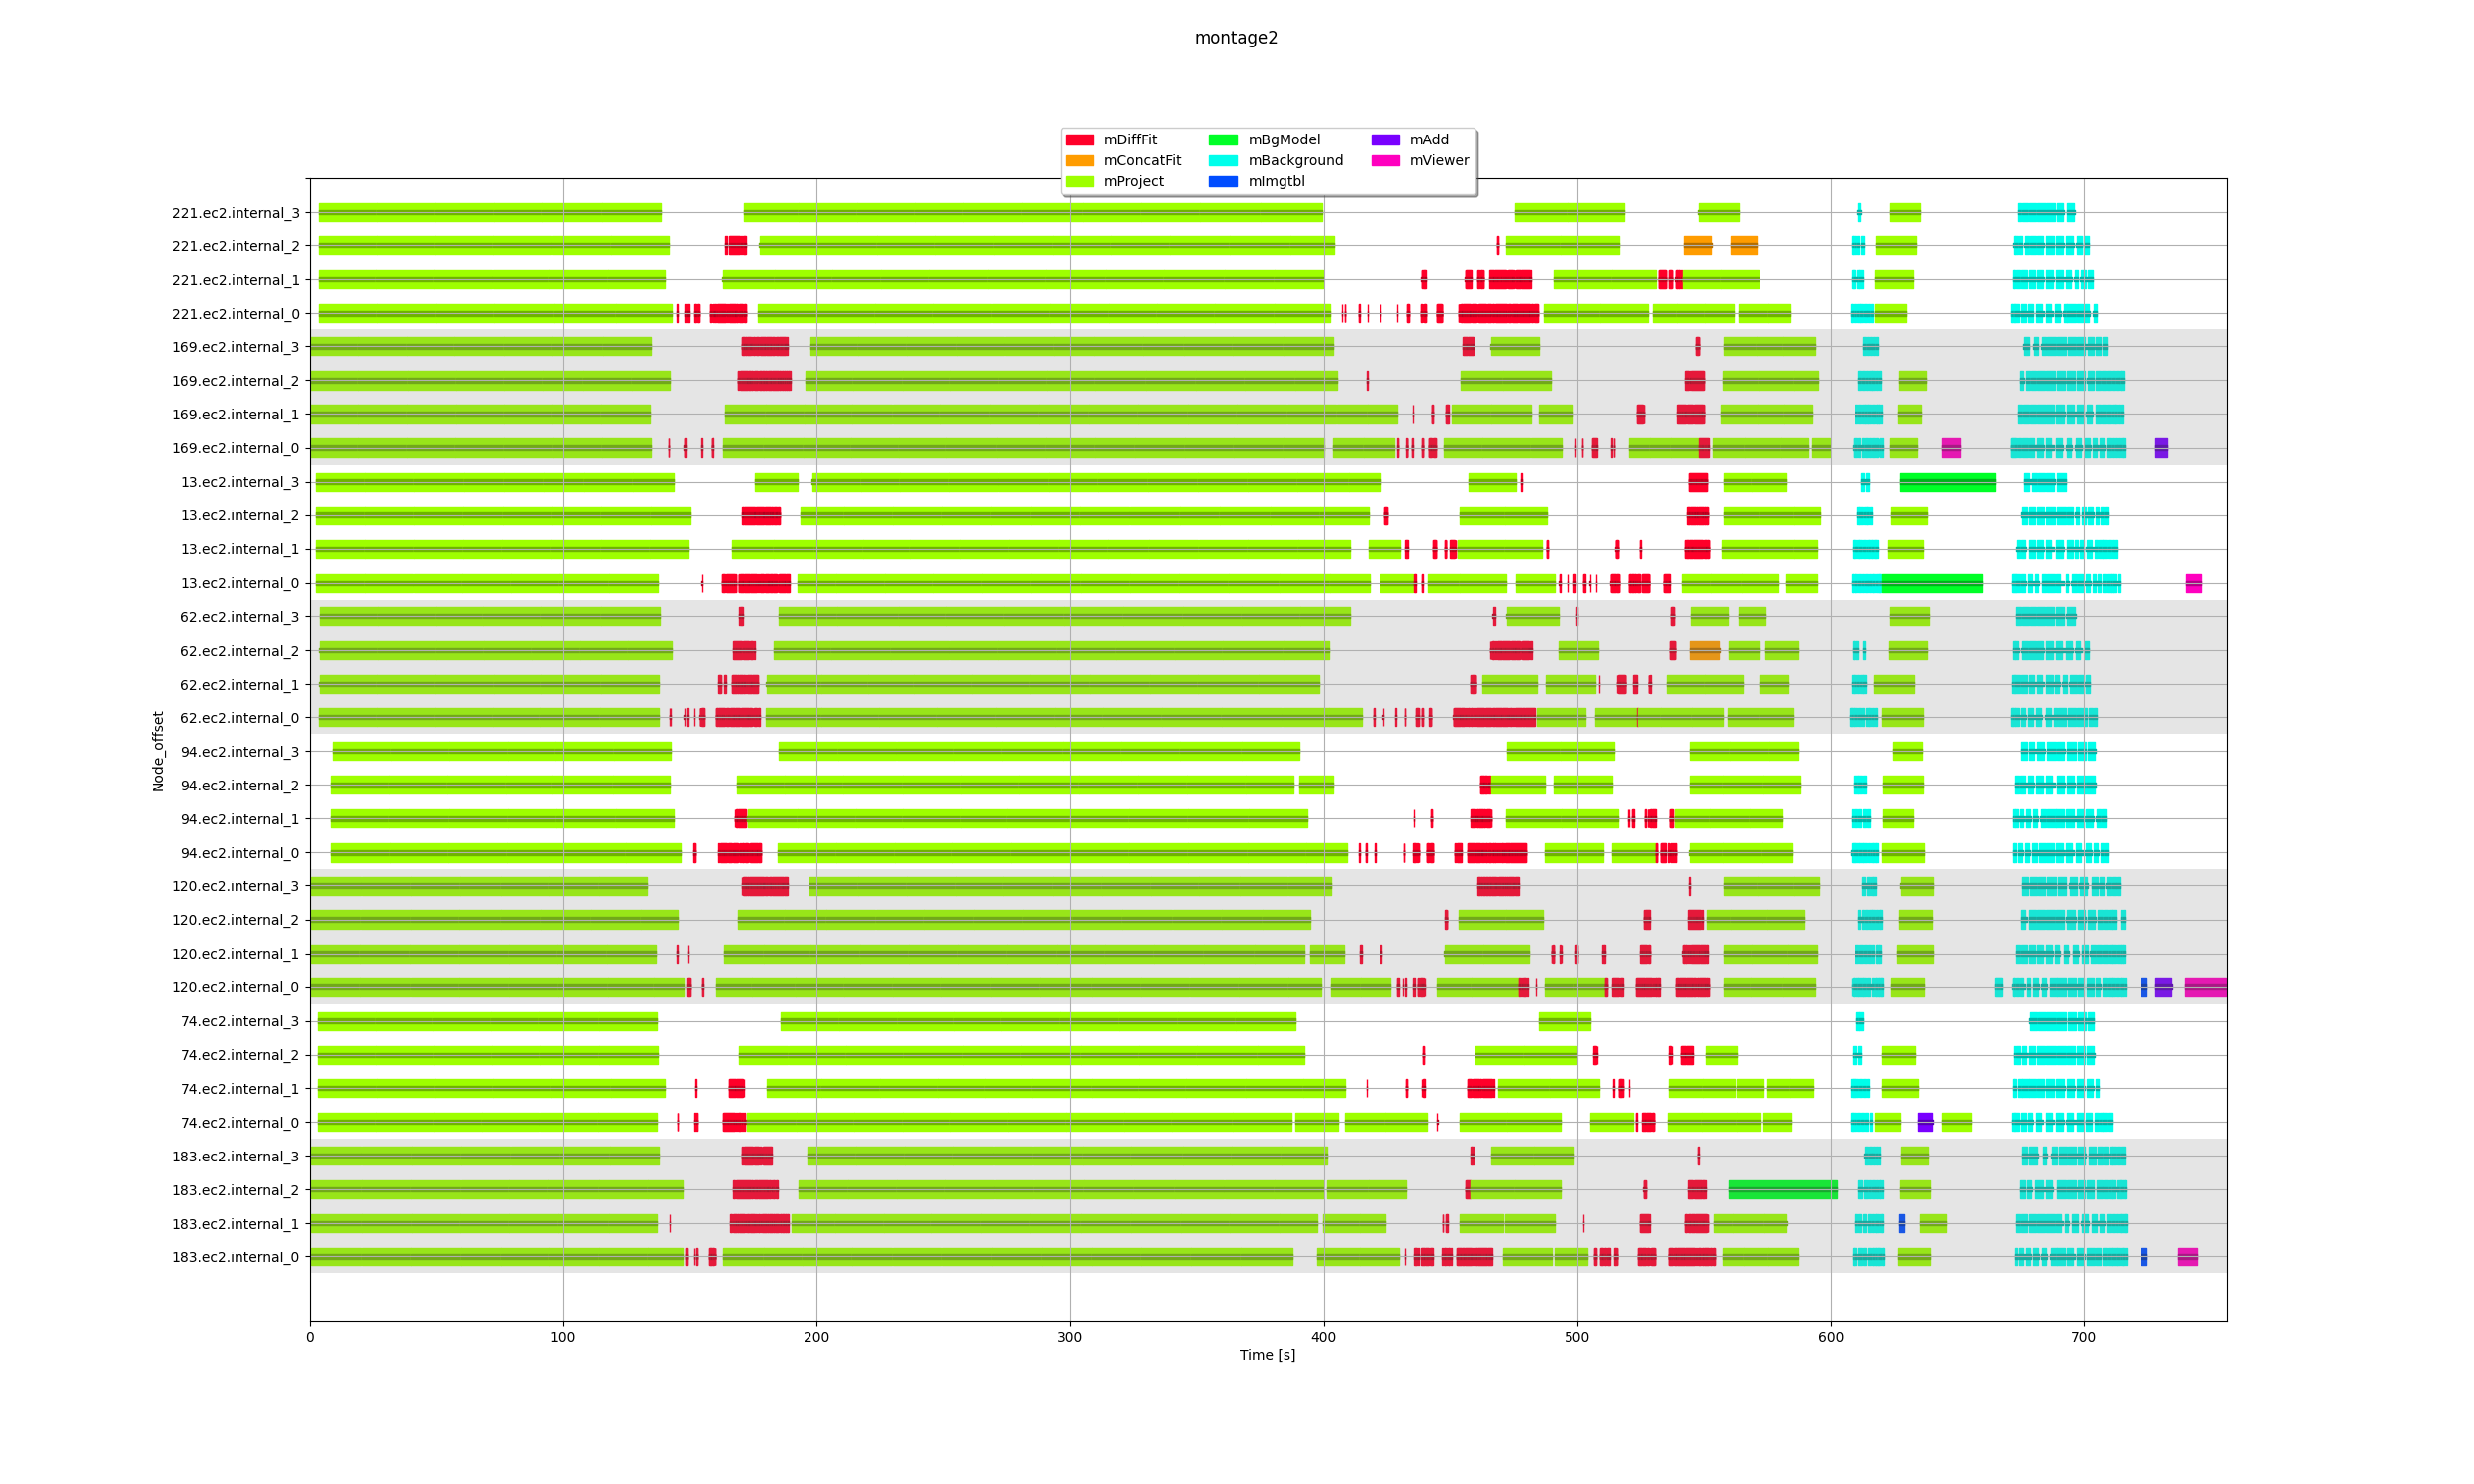
\includegraphics[width=1\linewidth]{figures/6-2-m1.0-agglo-peft.png}
% \caption[Task clustering on PEFT-planned schedule - Montage-1.0]{Task clustering on PEFT-planned schedule - Montage-1.0.}
% \label{fig:evaluation:agglo:m10:peft}
% \end{figure}
%%%%




%%%%%%%
\subsection{Utilization-based resource quota comparison}\label{s:Evaluation:ResourceOptimal}

% \todo{Experiments with task agglomeration and scheduling against a solution with optimal resource quotas}

The last scenario in the experimental process revolves around the optimal utilization of available node resources.
In previous scenarios, it has been assumed that each container is assigned a single processor.
This may have not fully reflected the capabilities of container computing as pods can have assigned partial resource quotas as well. 
This scenario has been prepared to make sure the performance of the default solution was not unintentionally affected in previous runs.
To compare the results from both scenarios, the Montage2-v1.0 workflow has been considered for this experiment.

As each pod in Kubernetes can have different resource quotas, it has been decided to adjust them to the values from appropriate measurements, based on the operation that is run by the tasks in this specific container.
Those measurements concentrate only on the CPU utilization, since any possible slowdown may have been caused only by improper management of this single resource.
In \cref{tab:res-util:setup} both the average usages measured and the actual assigned values are provided.
Some of the tasks have a reported utilization rate of zero, and to make a pod creation possible, a minimum CPU request has been introduced with two different values provided for this scenario.


% Tabelka z metrykami - Montage-1.0
\begin{table}[H]
    \centering
    \begin{tabular}{|c|c|c|c|c|}
    \cline{1-5}
        \multirow{2}{*}{Operation name} 
        &
        \multicolumn{2}{|c|}{Measured CPU usage}
        &
        \multicolumn{2}{|c|}{Assigned CPU request}  \\
    \cline{2-5}
        & m5.xlarge & m5a.xlarge & min CPU = 0.25 & min CPU = 0.50 \\
    \cline{1-5}
        mProject & 0.95 & 0.95 & \multicolumn{2}{|c|}{0.95} \\
    \cline{1-5}
        mDiffFit & 0.0 (!) & 0.0 (!) & 0.25 & 0.50 \\
    \cline{1-5}
        mConcatFit & 0.82 & 0.77 & \multicolumn{2}{|c|}{0.85} \\
    \cline{1-5}
        mBgModel & 1.00 & 1.00 & \multicolumn{2}{|c|}{1.00} \\
    \cline{1-5}
        mBackground & 0.0 (!) & 0.20 & 0.25 & 0.50 \\
    \cline{1-5}
        mImgtbl & 0.44 & 0.60 & \multicolumn{2}{|c|}{0.60} \\
    \cline{1-5}
        mAdd & 0.76 & 0.78 & \multicolumn{2}{|c|}{0.8} \\
    \cline{1-5}
        mViewer & 1.00 & 1.00 & \multicolumn{2}{|c|}{1.00} \\
    \cline{1-5}
    \end{tabular}
    \caption{Usages and CPU requests per workflow operation}
    \label{tab:res-util:setup}
\end{table}
%%%%


The execution traces for both setups are presented in \cref{fig:evaluation:res-util:m10:plugin}.
Adjusting CPU requests for pods resulted in an execution of up to six pods in parallel on nodes with only 4 vCPUs.
For a setup with a minimal CPU request of 0.5 vCPU, the utilization is nearly the same as with fixed CPU requests -- the parallelization of five pods occurs rarely and for a short time.
Only the other setup seems to really benefit from usage-based configuration.


%%%%%%%% Traces - Optimal
\begin{figure}[H]
\begin{subfigure}{1.0\textwidth}
\centering
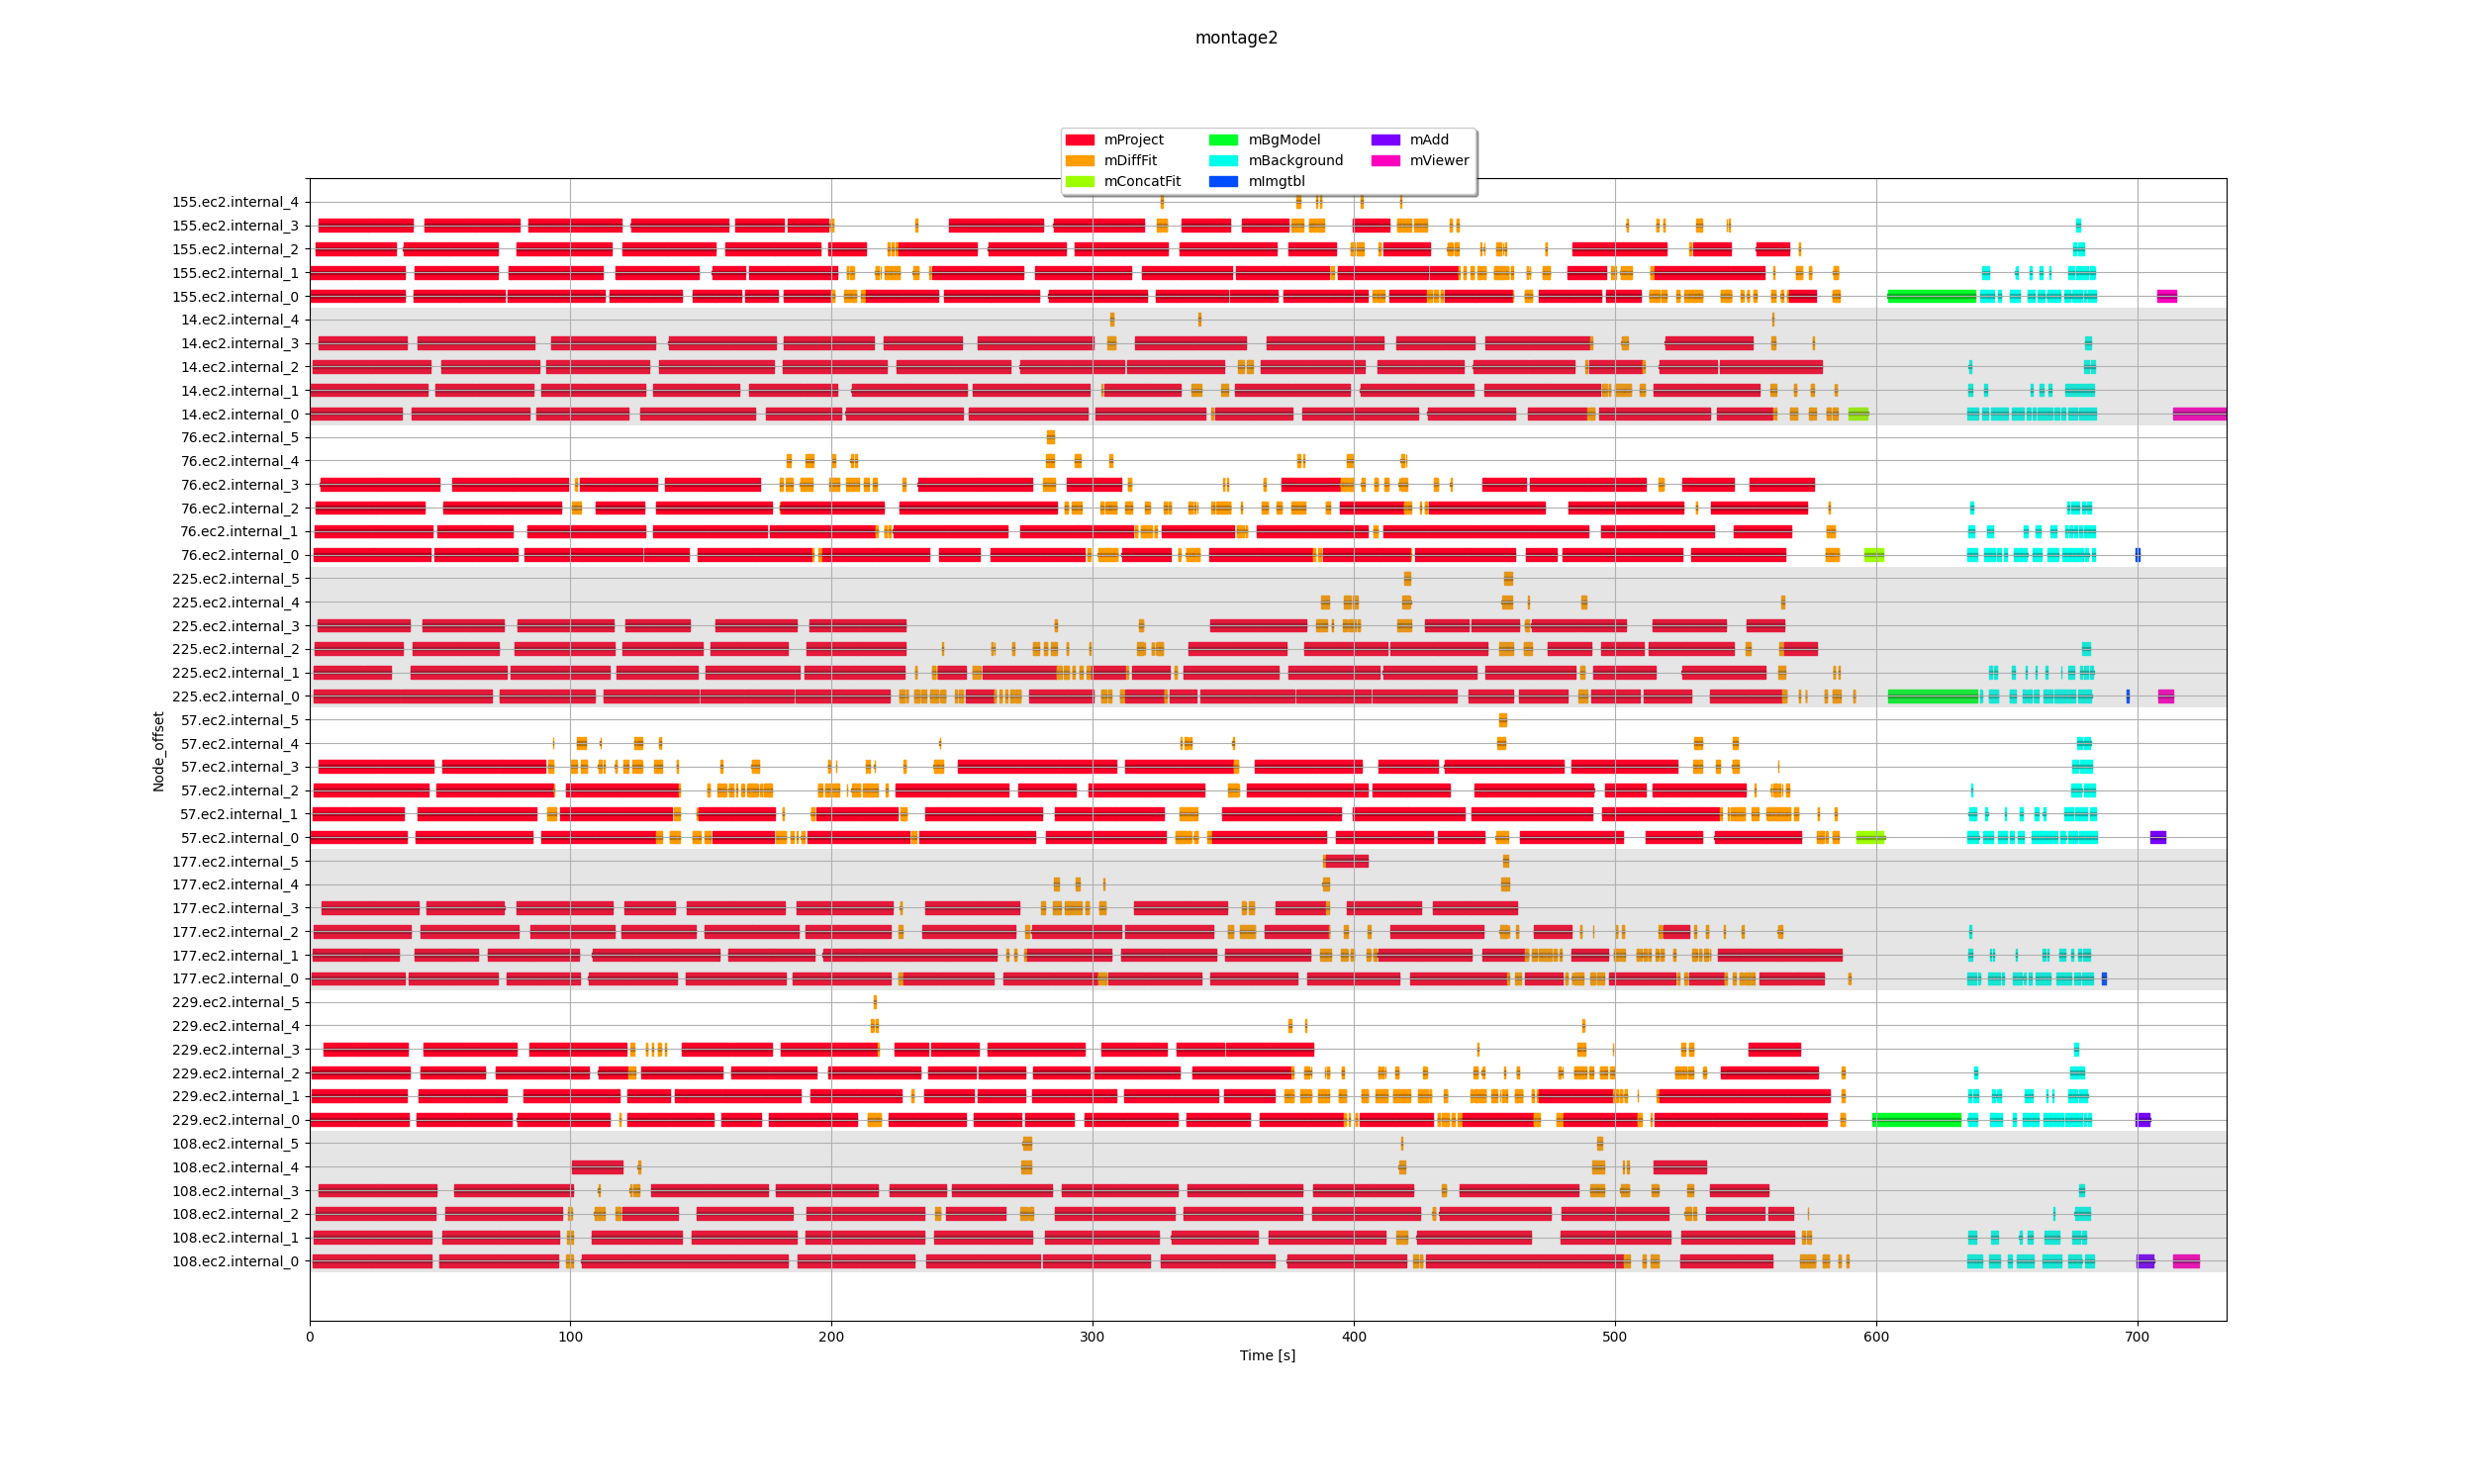
\includegraphics[width=1\linewidth]{figures/6-3-m1.0-optimal-cpu-0.25.png}
\caption[Selected example execution trace of Montage2-v1.0 with usage based CPU requests, min 0.25]{min CPU = 0.25}
\label{fig:evaluation:res-util:m10:025}
\end{subfigure}
\begin{subfigure}{1.0\textwidth}
\centering
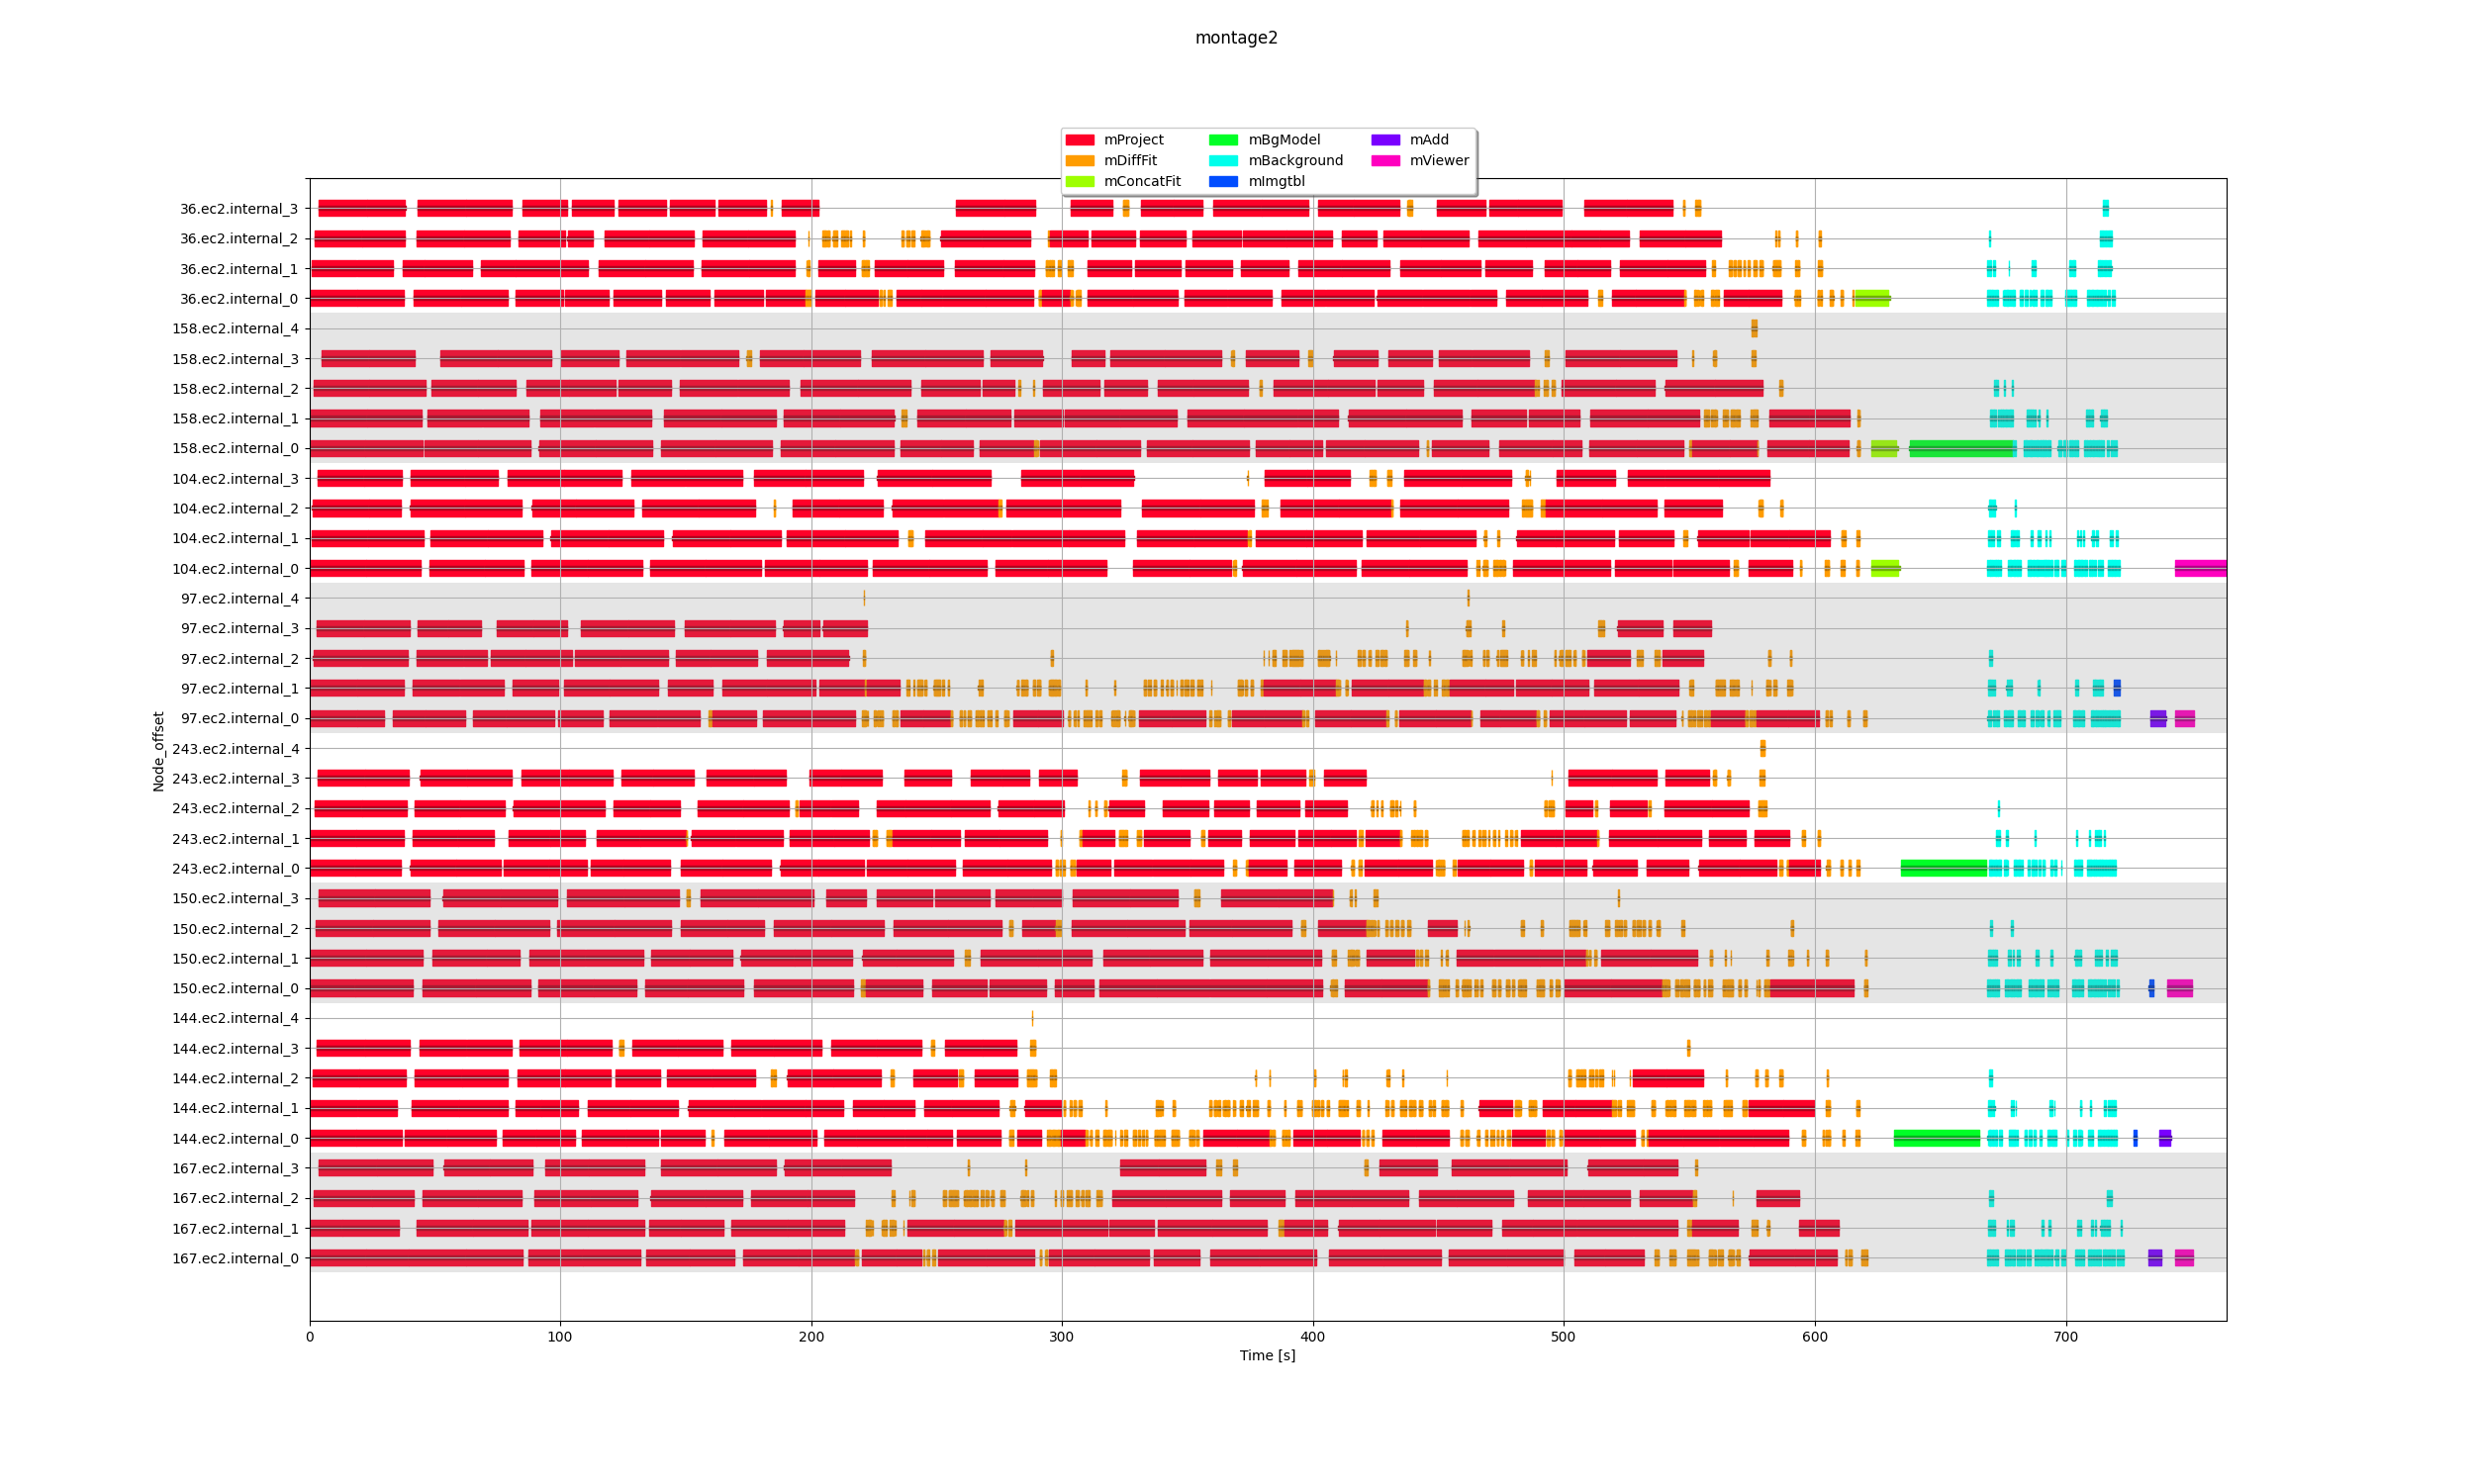
\includegraphics[width=1\linewidth]{figures/6-3-m1.0-optimal-cpu-0.50.png}
\caption[Selected example execution trace of Montage2-v1.0 with usage based CPU requests, min 0.50]{min CPU = 0.50}
\label{fig:evaluation:res-util:m10:050}
\end{subfigure}
\centering
%%
\caption[Selected example execution traces of Montage2-v1.0 with usage based CPU requests]{Selected example execution traces of Montage2-v1.0 with usage based CPU requests.}
\label{fig:evaluation:res-util:m10:plugin}
\end{figure}
%%%%%%%%


With the metrics provided in \cref{tab:res-util:results} it can be concluded that the final performance is highly dependant on the minimal CPU request.
It would, however, require to check all possible configurations to verify which setup performs the best with no guarantee for better results.


%%% Tabelka z metrykami - Optimal
\begin{table}[H]
    \centering
    \begin{tabular}{|c|c|c|c|c|c|}
    \cline{1-6}
        \multirow{2}{*}{Scenario} 
        &
        \multirow{2}{*}{Approach} 
        &
        \multicolumn{4}{|c|}{Metrics} \\
    \cline{3-6}
        & & Makespan & Job slowdown & SLR & CO \\
    \cline{1-6}
        \multirow{2}{*}{\vtop{\hbox{\strut\centering usage-based}\hbox{\strut\centering CPU requests}}} & min CPU = 0.25 & 746.7 & 48 & 7.27 & 12176 \\
    \cline{2-6}
        & min CPU = 0.50 & 779.1 & 243 & 7.55 & 15083 \\
    \cline{1-6}
        \multirow{3}{*}{\vtop{\hbox{\strut\centering fixed}\hbox{\strut\centering CPU requests}}} & kube-scheduler & 778.5 & 537 & 7.61 & 8200 \\
    \cline{2-6}
        & HEFT + kube-scheduler & 711.9 & 239 & 7.08 & 1271 \\
    \cline{2-6}
        & PEFT + kube-scheduler & 770.2 & 256 & 7.31 & 2008 \\
    \cline{1-6}
    \end{tabular}
    \caption{Comparison of metrics from Montage2-v1.0 execution from both scenarios}
    \label{tab:res-util:results}
\end{table}
%%%

The overall best solution for task clustering of all is still the HEFT schedule-based one.
For both utilization-based setups, the one with minimal CPU request set to 0.25 results in the better workflow execution efficiency.
It performs over 3\% better in terms of makespan reduction than PEFT and the default solution with fixed CPU requests.
Nonetheless, it is still behind the HEFT one, which has almost 5\% shorter execution times.


On the other hand, the utilization-based approach seems to achieve much better job slowdown.
As there is a higher chance for a pod to match its quota with the available resources in the cluster, the difference between time of arrival and time of task execution start lowers on average.
The only downside seems to be a higher containerization overhead, which seems to be one of the crucial aspects affecting the performance of this approach.
There is definitely a potential of improving the overall effectiveness of usage-based solutions if the lesser CO is achieved.


%%%%%%%
\subsection{Summary}

To sum up the results of the whole experiment, the two-step scheduling proves to be a more effective approach than the currently available solution, providing from 3\% to 10\% shorter execution times.
The only scenario that contradicts this statement is the execution of a workflow with a large number of short tasks.
When there is no task clustering enabled, all approaches seem to have a problem with workload parallelization.
This is an edge case of every solution and scheduling yields worse results in such situation.


Considering task clustering with two-step scheduling, it has been proven that it helps reducing the container overhead.
The more tasks in the workflow, the more it can benefit from such reduction in terms of shortening the execution time.


\clearpage

Lastly, considering the metrics used in the evaluation process, the SLR metric has not proved as useful as expected.
Although it often reflects the performance of the executed schedule, it can fail to do so sometimes, likely because task execution times do not include containerization times in contrast to makespan.
Such relative independence of both values might lead to skewed results.  
It does not bring that much insight to the final result analysis for such experiments.

% Based on the analysis

% Sched and scenarios:

% - reduction in CO with agglo scheduling confirmed - highly important for large workflows

% - optimal resource scenario - unclear as it seems to be rather sensitive with MIN\_REQ configuration - for the analyzed cases it is not as good as two-step sched 
